%%%%%%%%%%%%%%%%%%%%%%%%%%%%%%%%%%%%%%%%%%%%%%%%%%%%%%%%%%%%%%%%%%%%%%%%%%%%%%%%%%
\begin{frame}[fragile]\frametitle{}
\begin{center}
{\Large Background}\\

{till word2vec}

\end{center}
\end{frame}



%%%%%%%%%%%%%%%%%%%%%%%%%%%%%%%%%%%%%%%%%%%%%%%%%%%%%%%%%%%
\begin{frame}[fragile]\frametitle{How do we represent the meaning of a word?}
Definition: meaning (Webster dictionary)

\begin{itemize}
\item the idea that is represented by a word, phrase, etc.
\item the idea that a person wants to express by using  words, signs, etc.
\item the idea that is expressed in a work of writing, art, etc.  
\end{itemize}

Commonest linguistic way of thinking of meaning:

\begin{center}
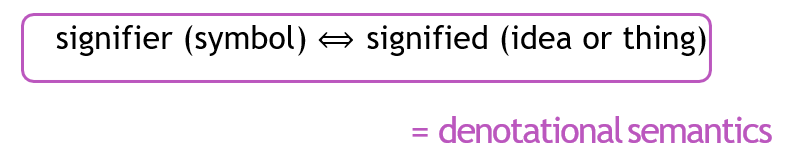
\includegraphics[width=0.6\linewidth,keepaspectratio]{bert2}
\end{center}		  

{\tiny (Ref: CS224n: Natural Language Processing with Deep Learning - Christopher Manning)}

\end{frame}


%%%%%%%%%%%%%%%%%%%%%%%%%%%%%%%%%%%%%%%%%%%%%%%%%%%%%%%%%%%
\begin{frame}[fragile]\frametitle{How do we have usable meaning in a computer?}


\begin{center}
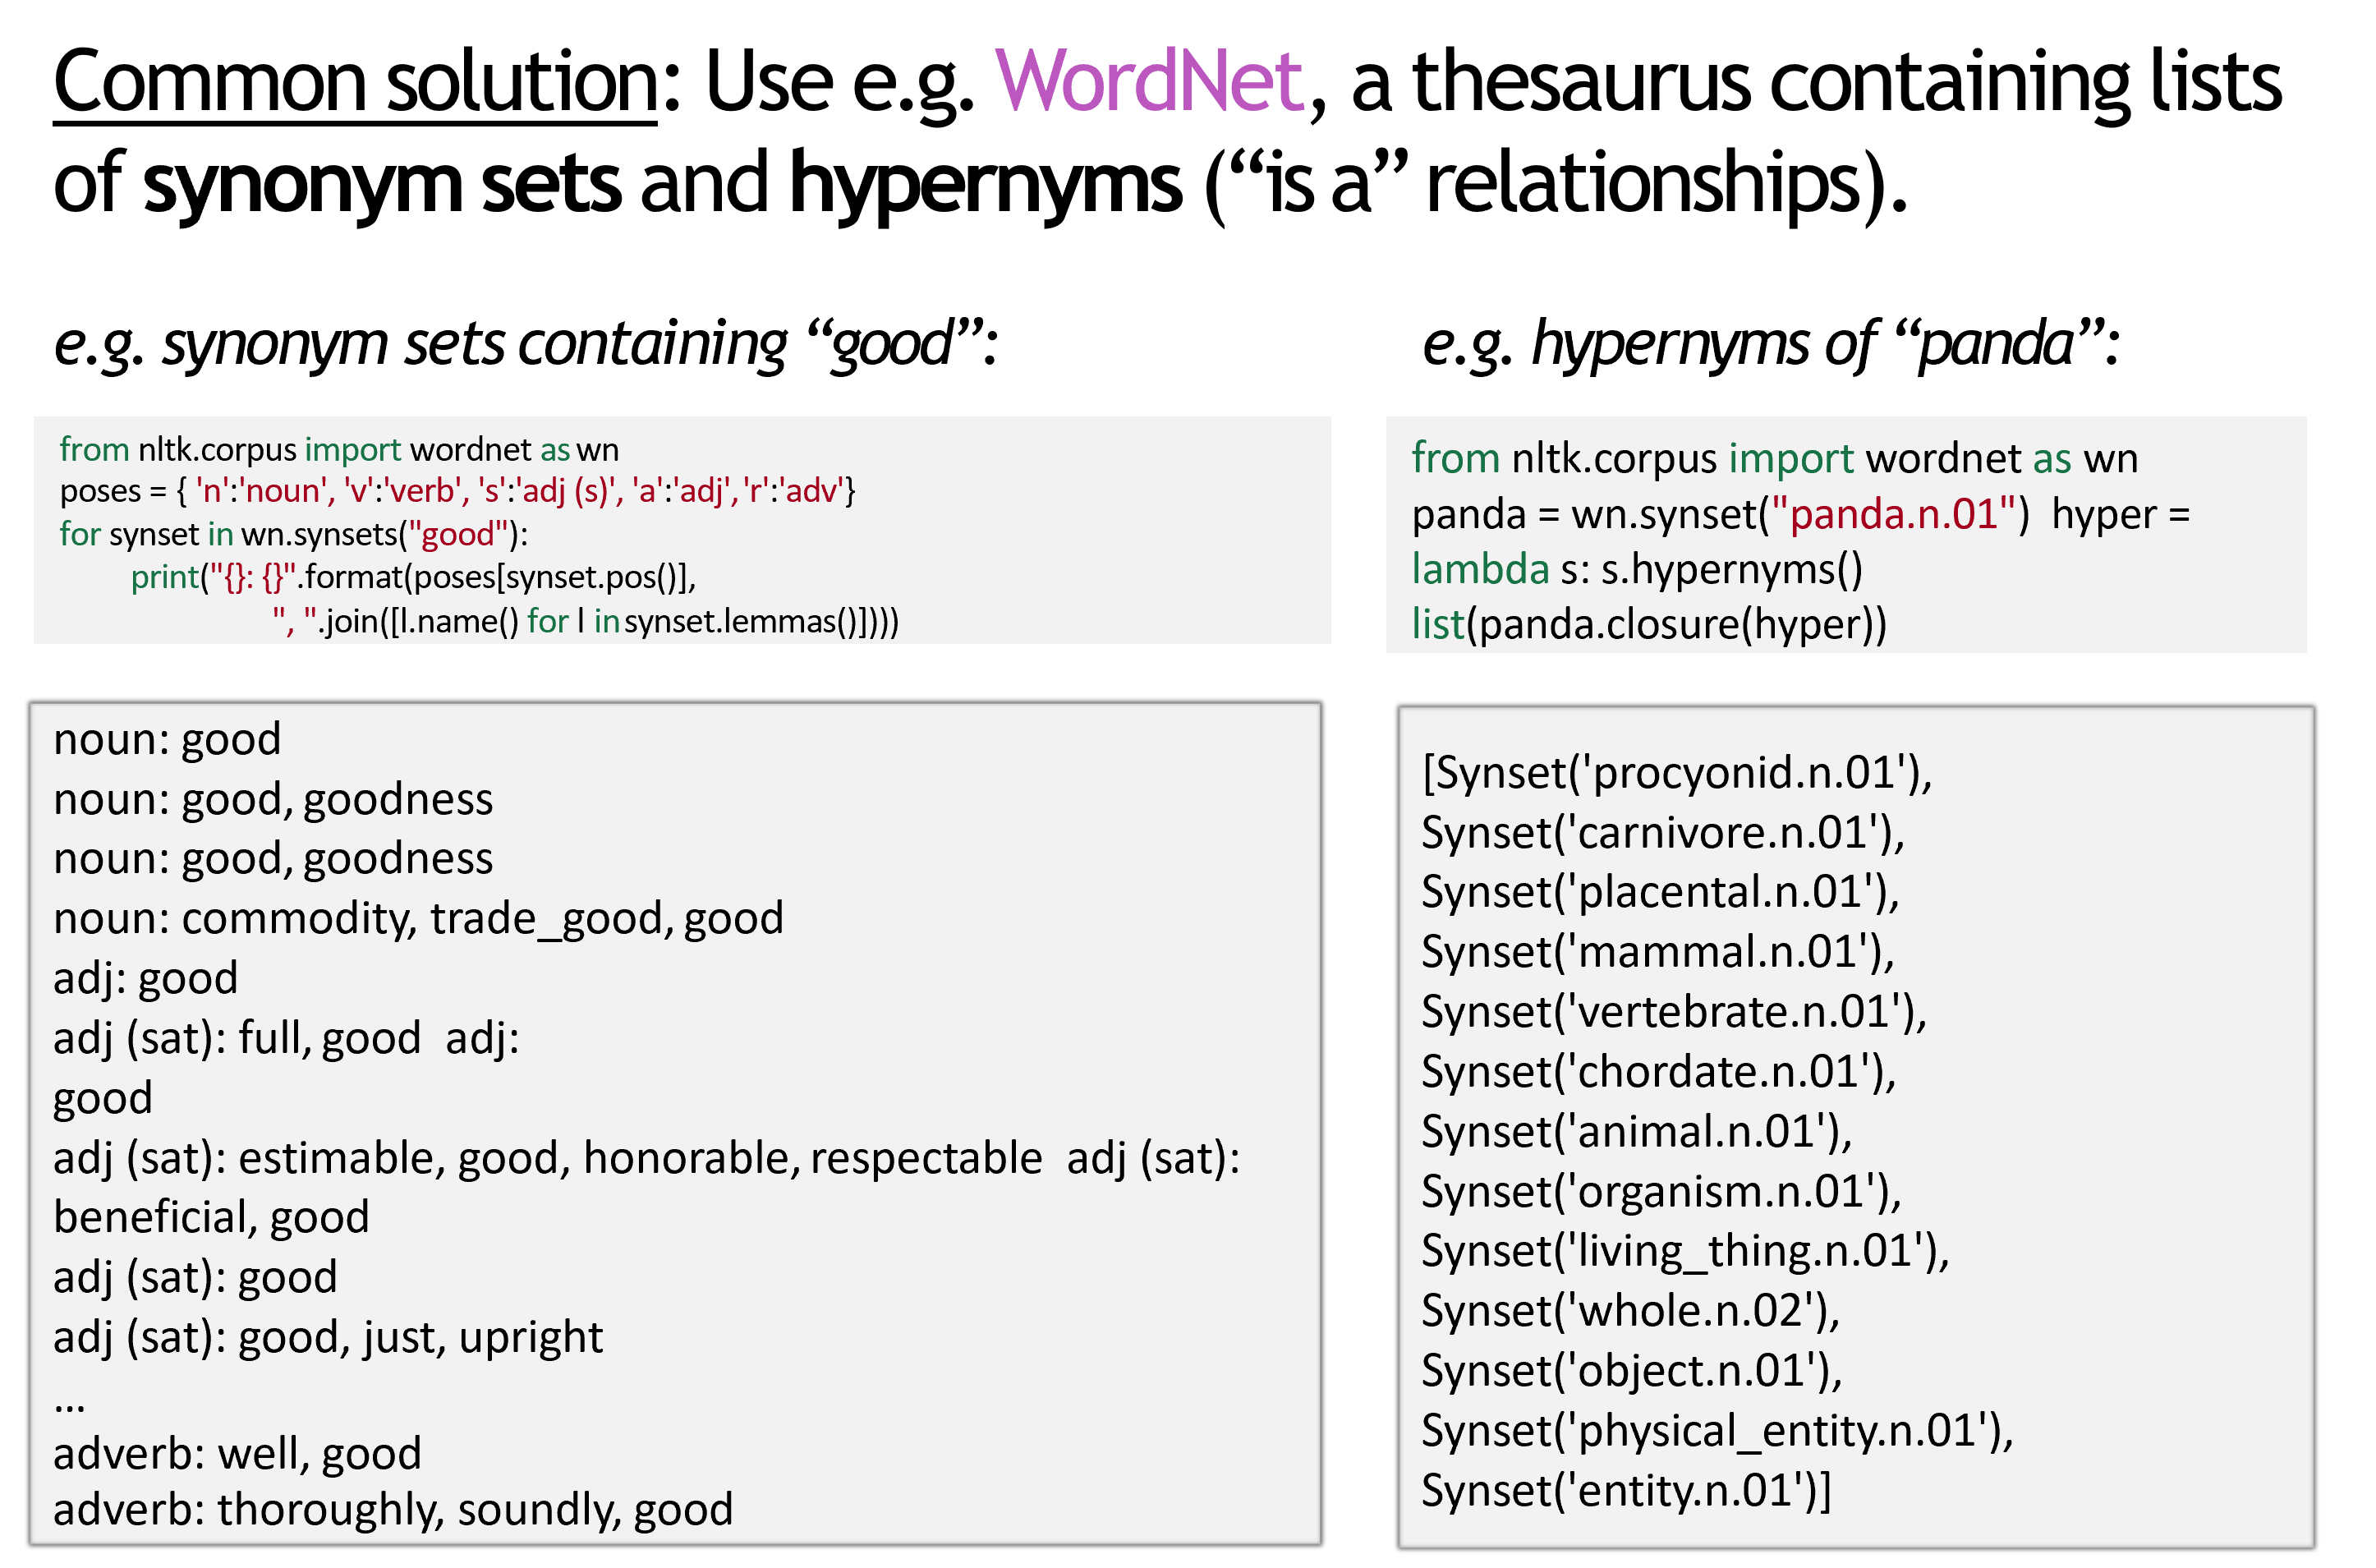
\includegraphics[width=\linewidth,keepaspectratio]{bert3}
\end{center}		  

{\tiny (Ref: CS224n: Natural Language Processing with Deep Learning - Christopher Manning)}

\end{frame}

%%%%%%%%%%%%%%%%%%%%%%%%%%%%%%%%%%%%%%%%%%%%%%%%%%%%%%%%%%%
\begin{frame}[fragile]\frametitle{Problems with resources like WordNet}


\begin{itemize}
\item Great as a resource but missing nuance: e.g. ``proficient'' is listed as a synonym for ``good''.  This is only correct in some contexts.
\item Missing new meanings of words: e.g., wicked, badass, nifty, wizard, genius, ninja, bombest. Impossible to keep up-to-date!
\item Subjective
\item Requires human labor to create and adapt
\item Can't compute accurate word similarity 
\end{itemize}

{\tiny (Ref: CS224n: Natural Language Processing with Deep Learning - Christopher Manning)}

\end{frame}

%%%%%%%%%%%%%%%%%%%%%%%%%%%%%%%%%%%%%%%%%%%%%%%%%%%%%%%%%%%
\begin{frame}[fragile]\frametitle{Representing words as discrete symbols}


\begin{center}
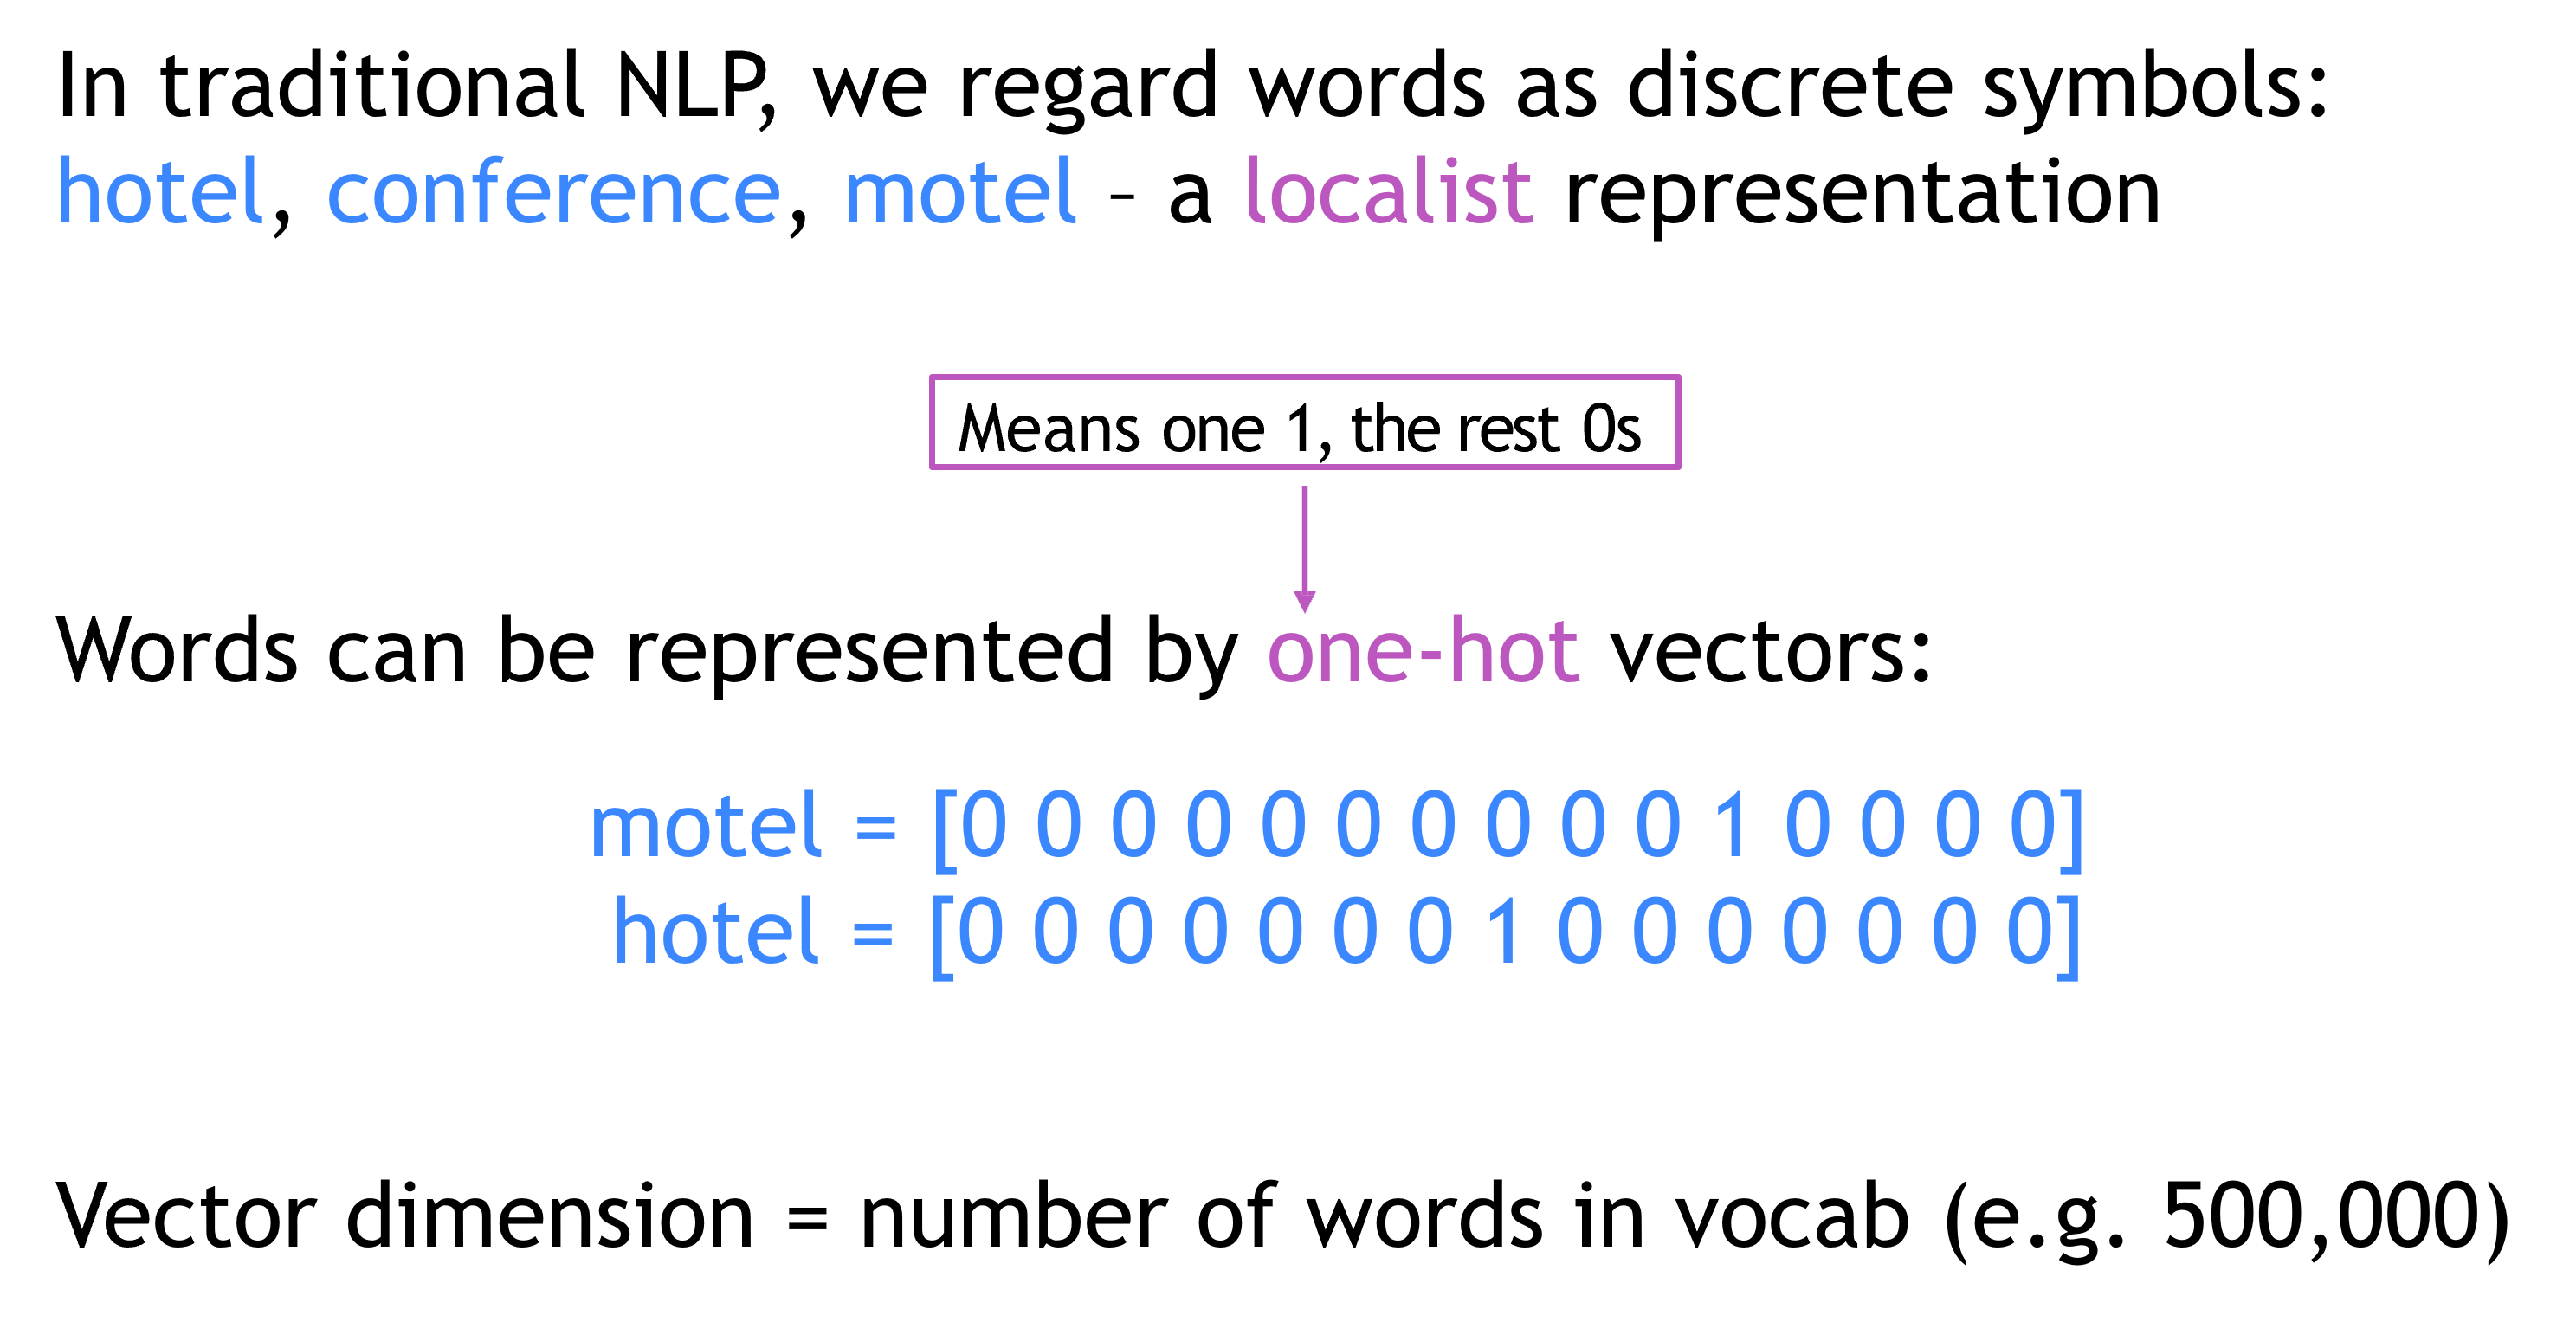
\includegraphics[width=\linewidth,keepaspectratio]{bert4}
\end{center}		  


{\tiny (Ref: CS224n: Natural Language Processing with Deep Learning - Christopher Manning)}

\end{frame}

%%%%%%%%%%%%%%%%%%%%%%%%%%%%%%%%%%%%%%%%%%%%%%%%%%%%%%%%%%%
\begin{frame}[fragile]\frametitle{Representing words as discrete symbols}


\begin{center}
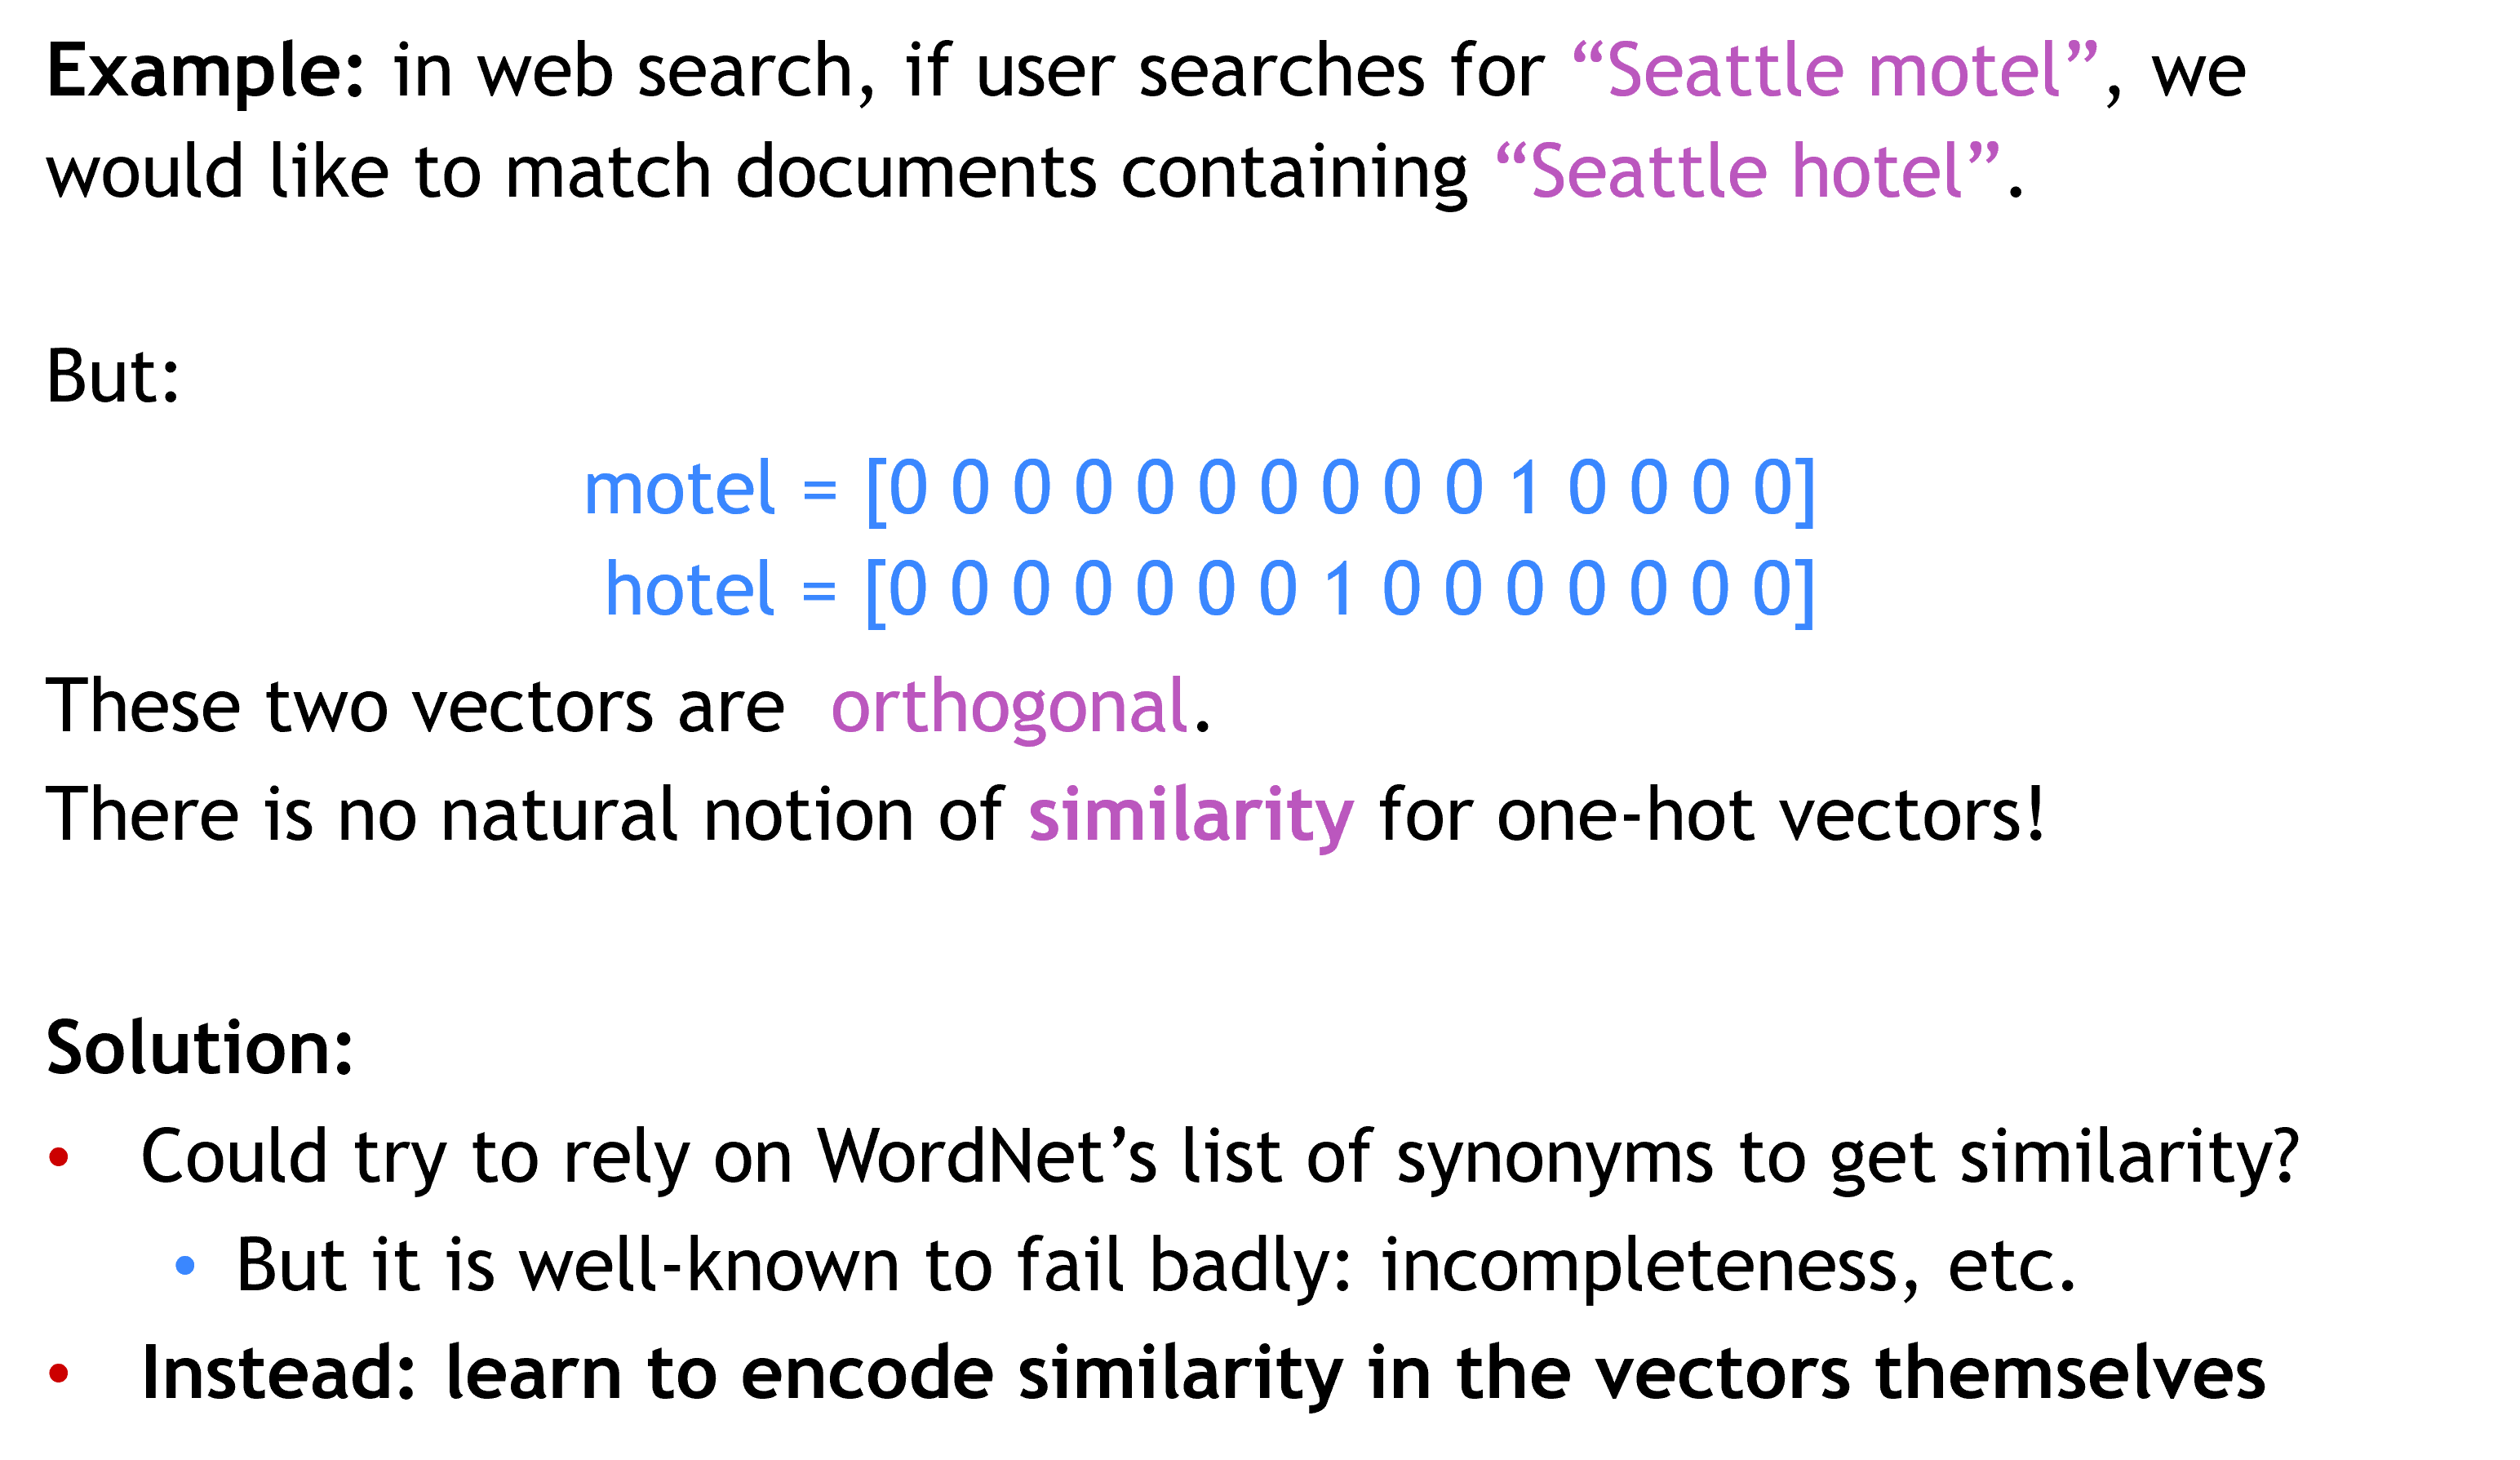
\includegraphics[width=\linewidth,keepaspectratio]{bert5}
\end{center}		  


{\tiny (Ref: CS224n: Natural Language Processing with Deep Learning - Christopher Manning)}

\end{frame}

%%%%%%%%%%%%%%%%%%%%%%%%%%%%%%%%%%%%%%%%%%%%%%%%%%%%%%%%%%%
\begin{frame}[fragile]\frametitle{Representing words by their context}


\begin{center}
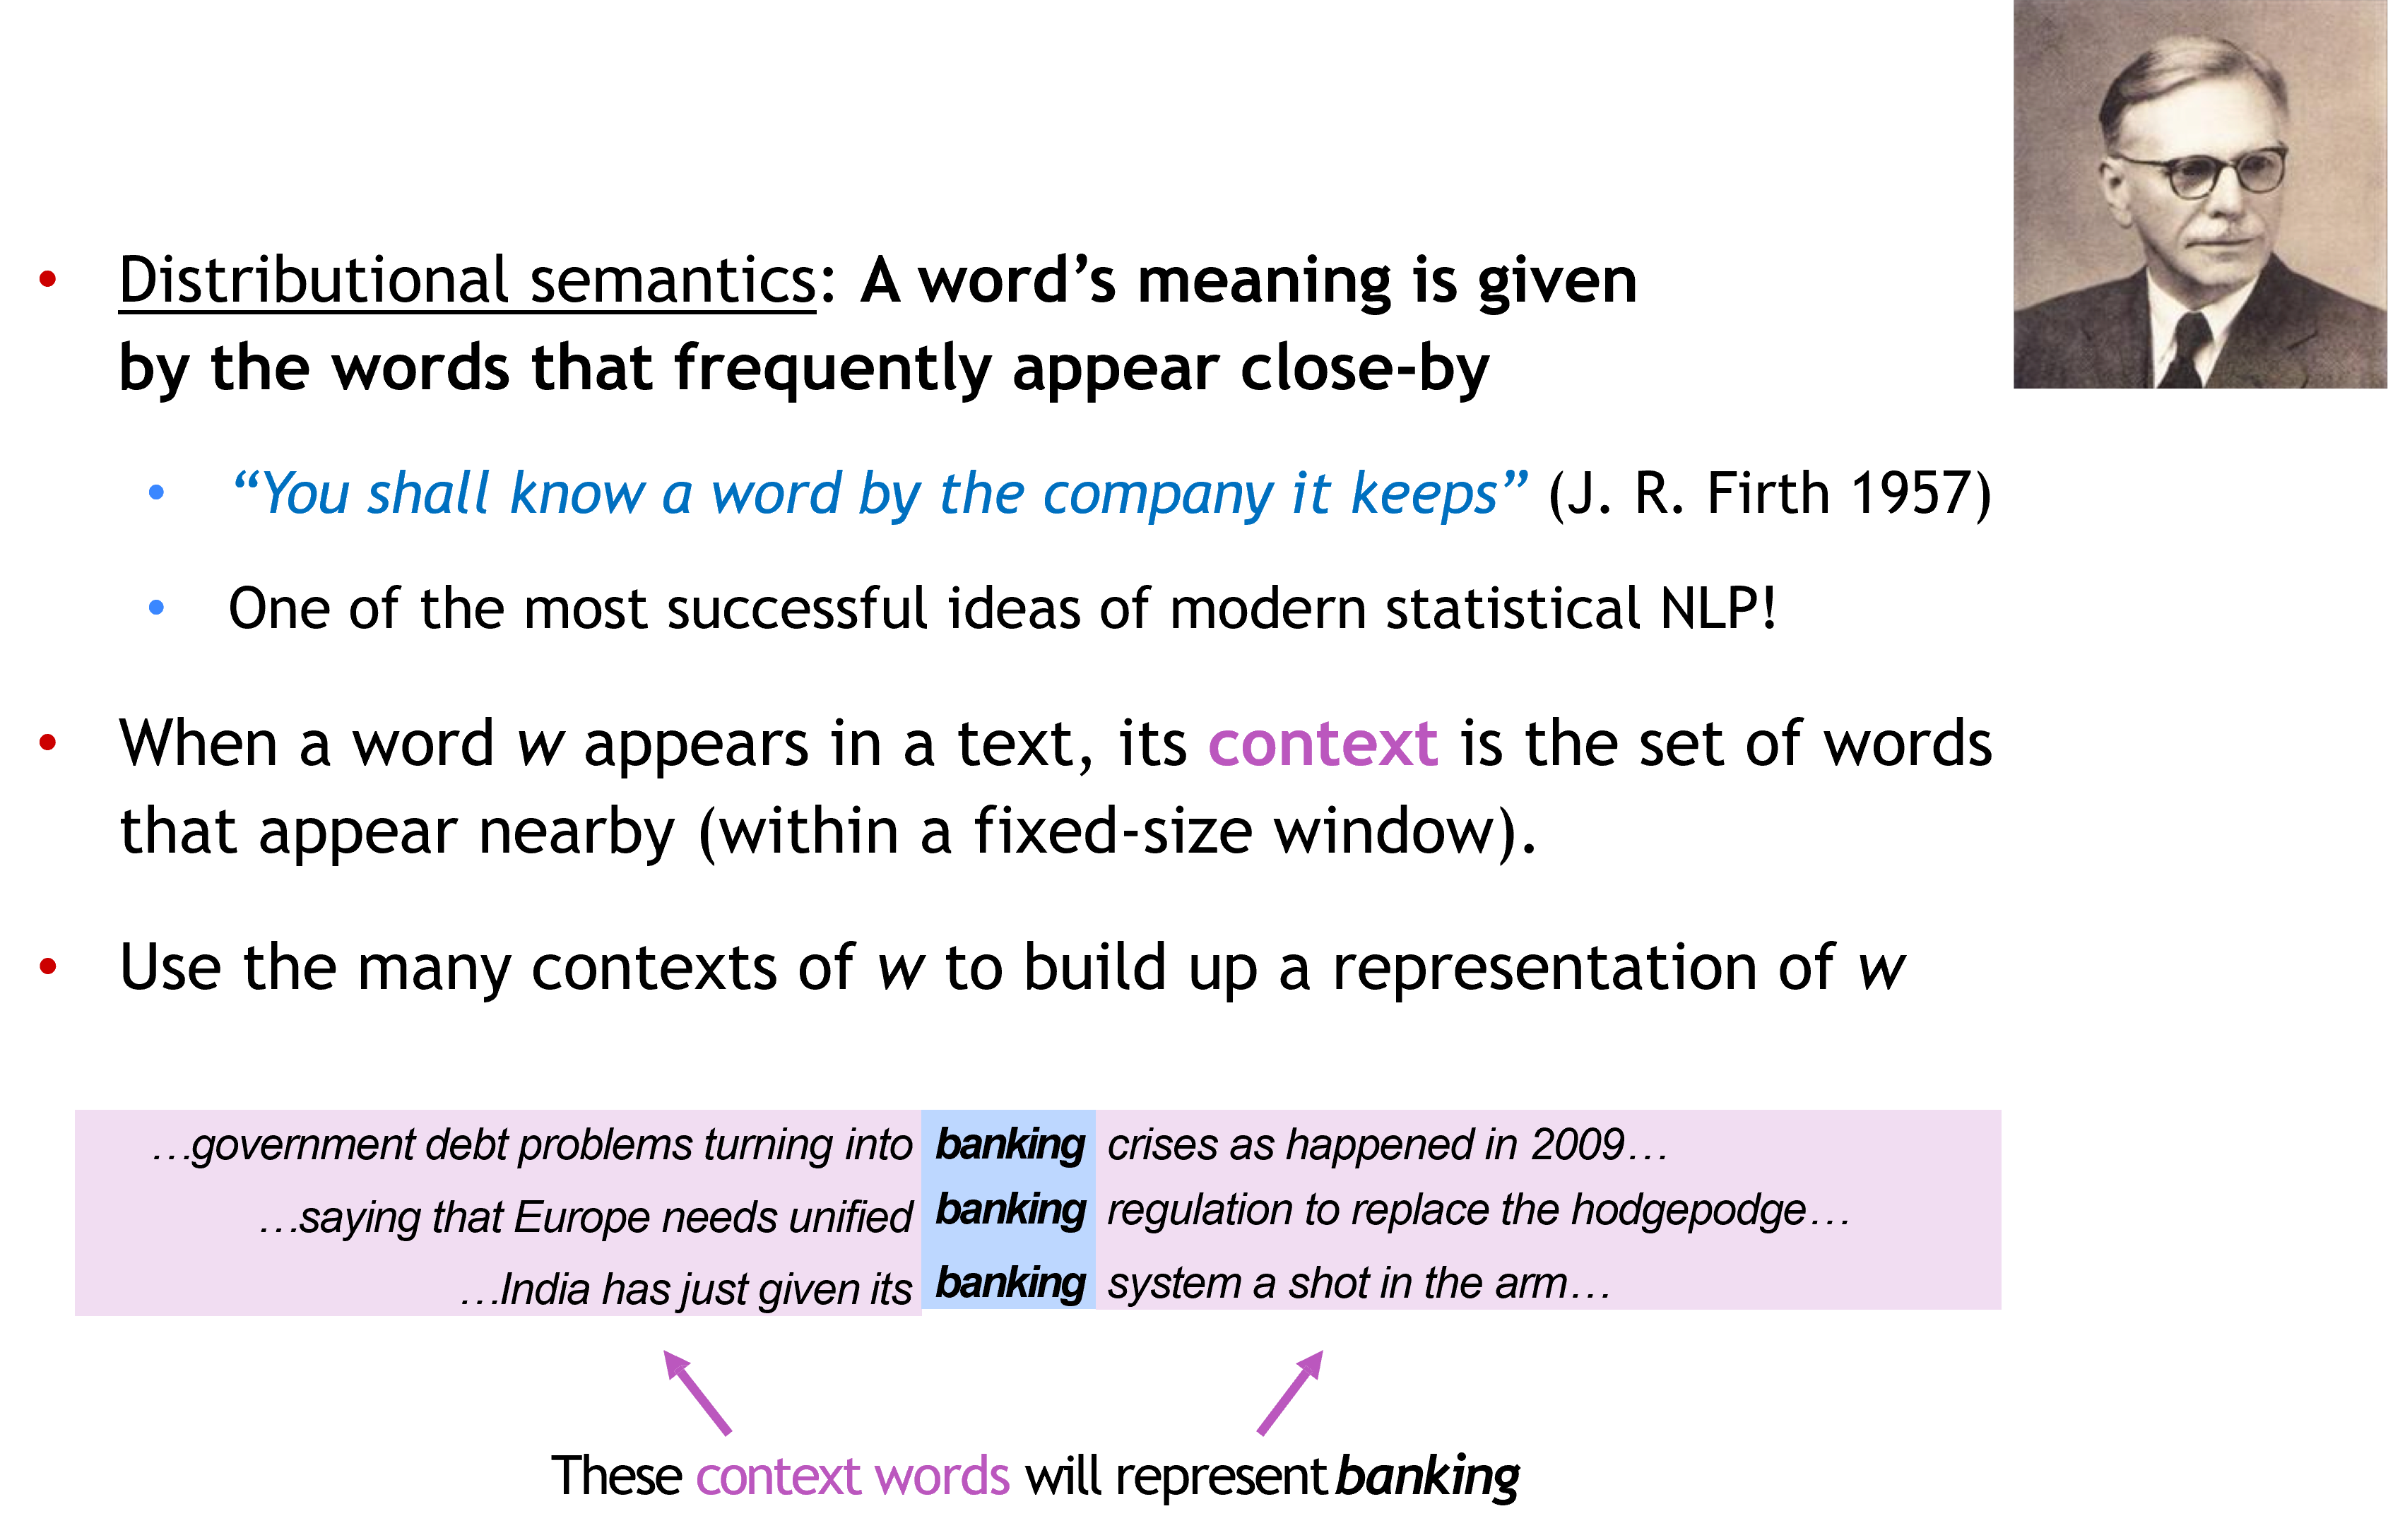
\includegraphics[width=\linewidth,keepaspectratio]{bert6}
\end{center}		  


{\tiny (Ref: CS224n: Natural Language Processing with Deep Learning - Christopher Manning)}

\end{frame}

%%%%%%%%%%%%%%%%%%%%%%%%%%%%%%%%%%%%%%%%%%%%%%%%%%%%%%%%%%%
\begin{frame}[fragile]\frametitle{What can we learn from reconstructing input?}

\begin{center}
Stanford University is located in $---------$	, California.
\end{center}		  

{\tiny (Ref: Language \& Machine Learning - John Hewitt)}
\end{frame}

%%%%%%%%%%%%%%%%%%%%%%%%%%%%%%%%%%%%%%%%%%%%%%%%%%%%%%%%%%%
\begin{frame}[fragile]\frametitle{What can we learn from reconstructing input?}

\begin{center}
I put $----------$ fork down on the table.
\end{center}		  

{\tiny (Ref: Language \& Machine Learning - John Hewitt)}
\end{frame}

%%%%%%%%%%%%%%%%%%%%%%%%%%%%%%%%%%%%%%%%%%%%%%%%%%%%%%%%%%%
\begin{frame}[fragile]\frametitle{What can we learn from reconstructing input?}

\begin{center}
The woman walked across the street, \\ checking for traffic over $----------$ shoulder.
\end{center}		  

{\tiny (Ref: Language \& Machine Learning - John Hewitt)}
\end{frame}

%%%%%%%%%%%%%%%%%%%%%%%%%%%%%%%%%%%%%%%%%%%%%%%%%%%%%%%%%%%
\begin{frame}[fragile]\frametitle{What can we learn from reconstructing input?}

\begin{center}
I went to the ocean to see the fish, turtles, seals, and $----------$.
\end{center}		  

{\tiny (Ref: Language \& Machine Learning - John Hewitt)}
\end{frame}

%%%%%%%%%%%%%%%%%%%%%%%%%%%%%%%%%%%%%%%%%%%%%%%%%%%%%%%%%%%
\begin{frame}[fragile]\frametitle{What can we learn from reconstructing input?}

\begin{center}
Overall, the value I got from the two hours watching \\ it was the sum total of the popcorn and the drink.\\
The movie was  $----------$.
\end{center}		  

{\tiny (Ref: Language \& Machine Learning - John Hewitt)}
\end{frame}

%%%%%%%%%%%%%%%%%%%%%%%%%%%%%%%%%%%%%%%%%%%%%%%%%%%%%%%%%%%
\begin{frame}[fragile]\frametitle{What can we learn from reconstructing input?}

\begin{center}
Iroh went into the kitchen to make some tea.\\
Standing next to Iroh, Zuko pondered his destiny.\\
Zuko left the  $----------$.
\end{center}		  

{\tiny (Ref: Language \& Machine Learning - John Hewitt)}
\end{frame}

%%%%%%%%%%%%%%%%%%%%%%%%%%%%%%%%%%%%%%%%%%%%%%%%%%%%%%%%%%%
\begin{frame}[fragile]\frametitle{What can we learn from reconstructing input?}

\begin{center}
I was thinking about the sequence that goes  \\ 1, 1, 2, 3, 5, 8, 13, 21,   $----------$.
\end{center}		  

{\tiny (Ref: Language \& Machine Learning - John Hewitt)}
\end{frame}

%%%%%%%%%%%%%%%%%%%%%%%%%%%%%%%%%%%%%%%%%%%%%%%%%%%%%%%%%%%
\begin{frame}[fragile]\frametitle{Word vectors}

We will build a dense vector for each word, chosen so that it is  similar to vectors of words that appear in similar contexts
	  
\begin{center}
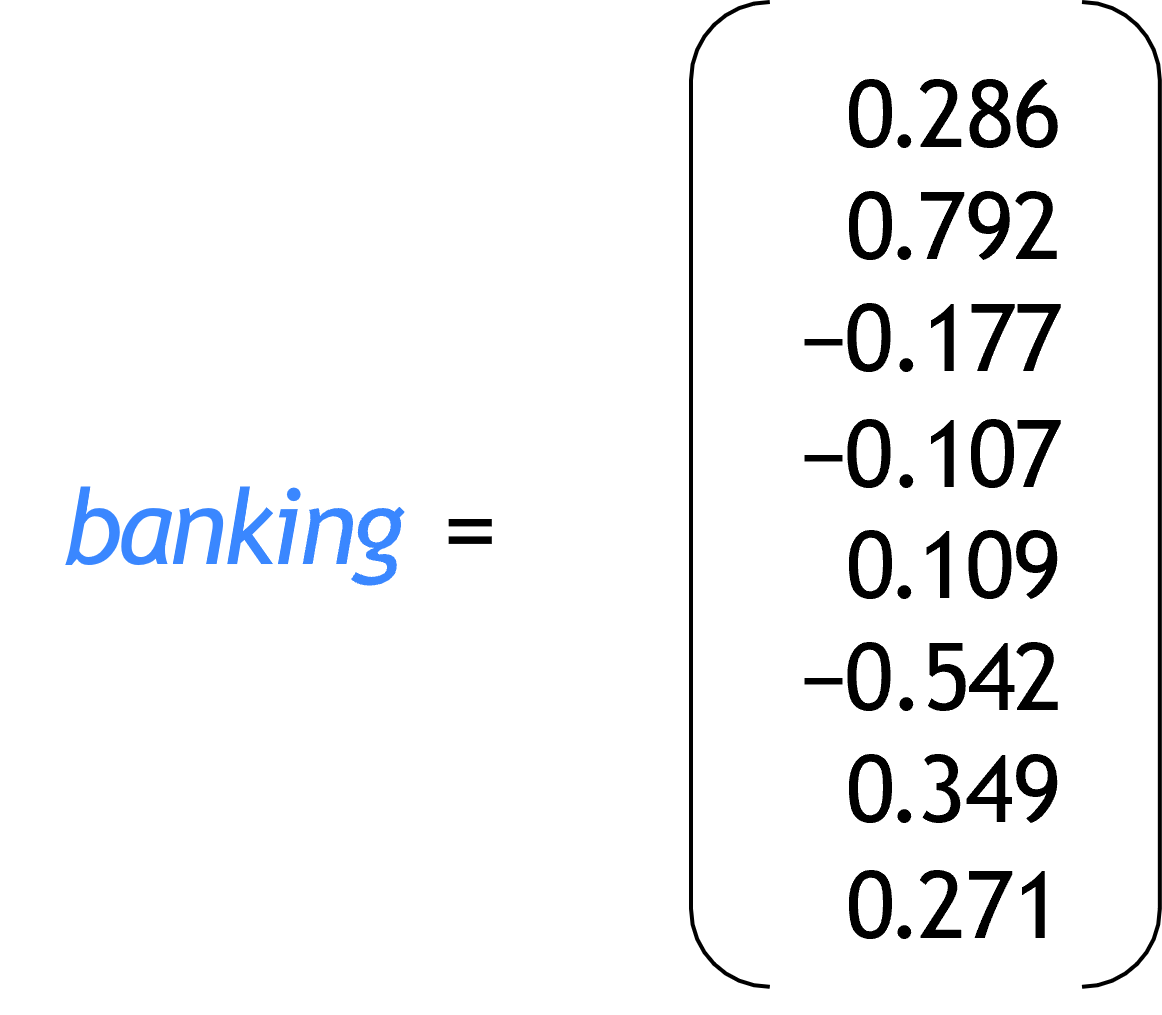
\includegraphics[width=0.5\linewidth,keepaspectratio]{bert7}
\end{center}		  
		
Note: word vectors are sometimes called word embeddings or  word representations. They are a distributed representation.

{\tiny (Ref: CS224n: Natural Language Processing with Deep Learning - Christopher Manning)}

\end{frame}

%%%%%%%%%%%%%%%%%%%%%%%%%%%%%%%%%%%%%%%%%%%%%%%%%%%%%%%%%%%
\begin{frame}[fragile]\frametitle{Word meaning as a neural word vector: visualization}

	  
\begin{center}
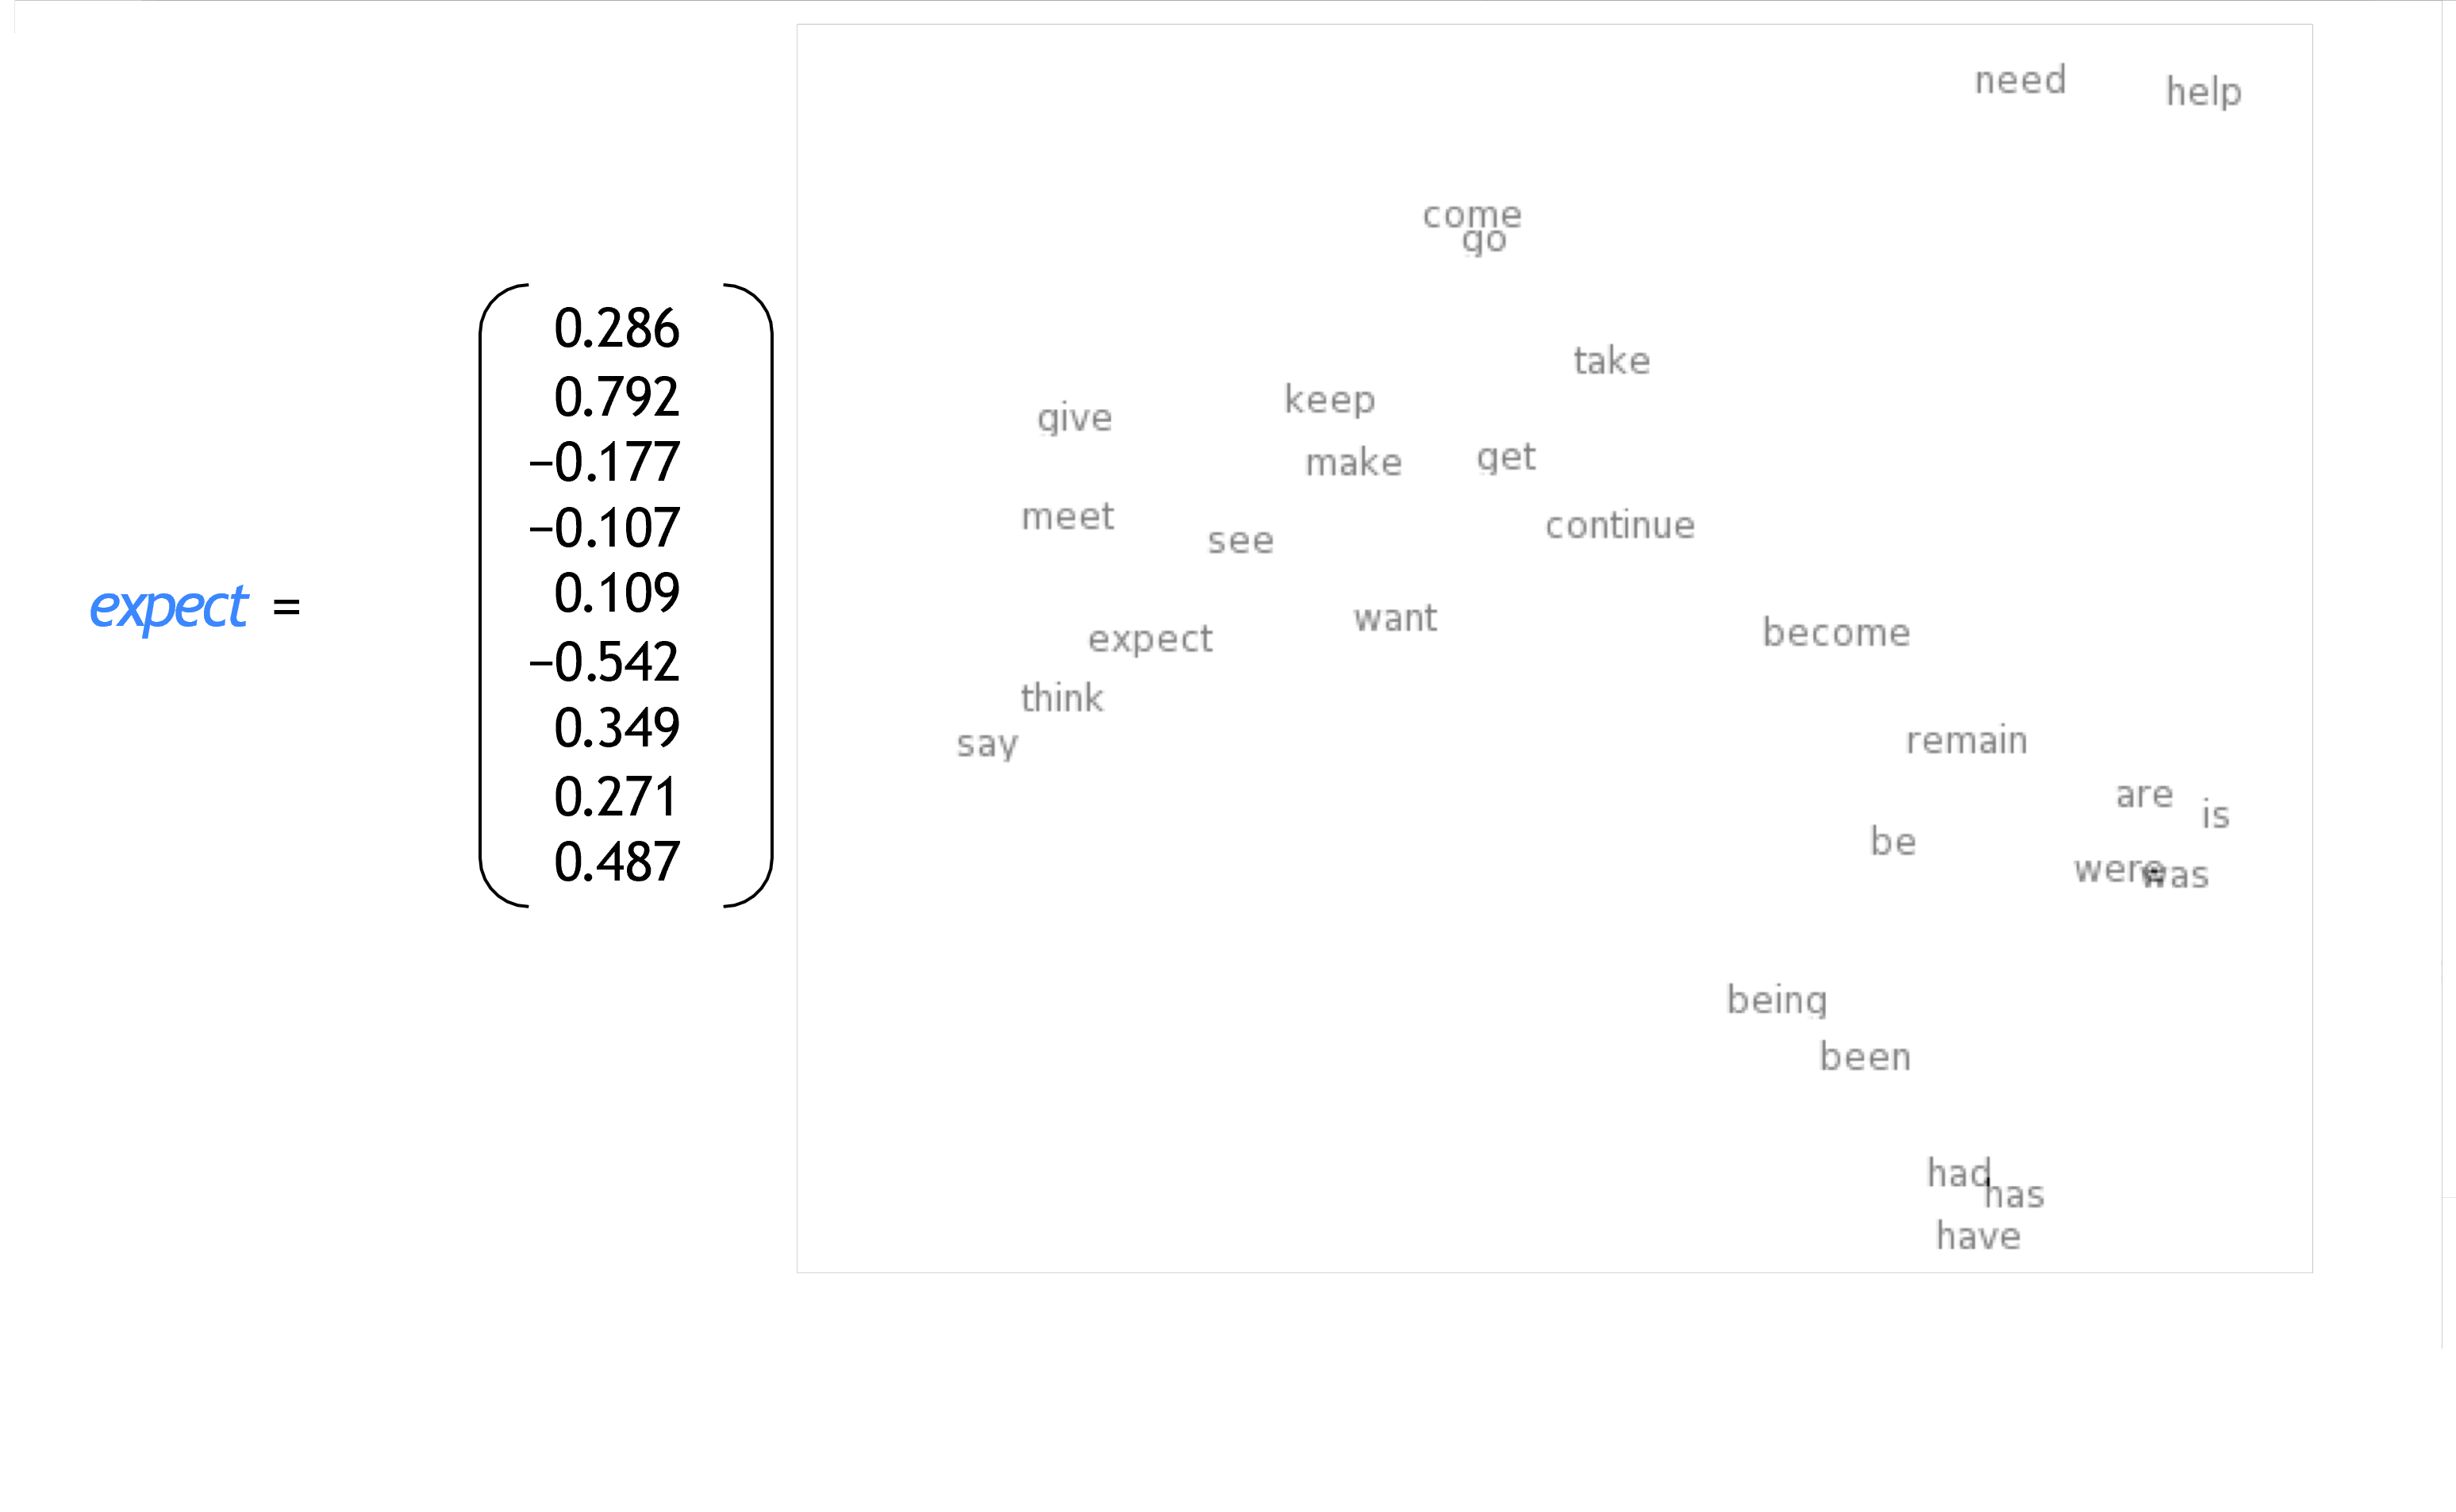
\includegraphics[width=\linewidth,keepaspectratio]{bert8}
\end{center}		  
		

{\tiny (Ref: CS224n: Natural Language Processing with Deep Learning - Christopher Manning)}

\end{frame}

%%%%%%%%%%%%%%%%%%%%%%%%%%%%%%%%%%%%%%%%%%%%%%%%%%%%%%%%%%%
\begin{frame}[fragile]\frametitle{Word2Vec Overview}
Word2vec (Mikolov et al. 2013) is a framework for learning  word vectors

Idea:
\begin{itemize}
\item We have a large corpus of text
\item Every word in a fixed vocabulary is represented by a vector
\item Go through each position t in the text, which has a center word
c and context (“outside”) words o
\item Use the similarity of the word vectors for c and o to calculate  the probability of o given c (or vice versa)
\item Keep adjusting the word vectors to maximize this probability

\end{itemize}

{\tiny (Ref: CS224n: Natural Language Processing with Deep Learning - Christopher Manning)}

\end{frame}

%%%%%%%%%%%%%%%%%%%%%%%%%%%%%%%%%%%%%%%%%%%%%%%%%%%%%%%%%%%
\begin{frame}[fragile]\frametitle{Word2Vec Overview}
Example windows and process for computing  $P(w_{t+j}|w_t)$


\begin{center}
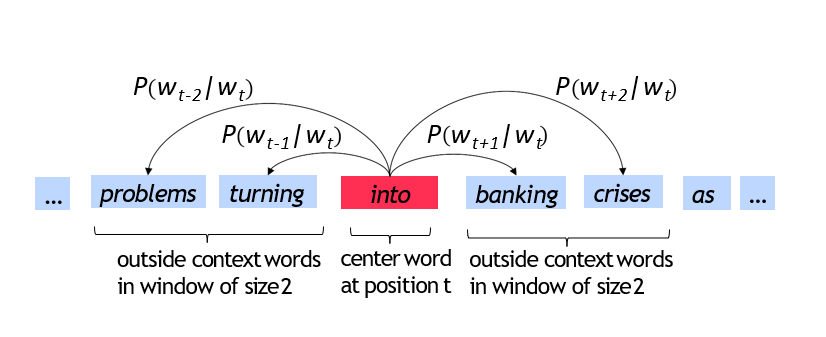
\includegraphics[width=\linewidth,keepaspectratio]{bert9}
\end{center}	

{\tiny (Ref: CS224n: Natural Language Processing with Deep Learning - Christopher Manning)}

\end{frame}

%%%%%%%%%%%%%%%%%%%%%%%%%%%%%%%%%%%%%%%%%%%%%%%%%%%%%%%%%%%
\begin{frame}[fragile]\frametitle{Word2Vec Overview}
Example windows and process for computing  $P(w_{t+j}|w_t)$


\begin{center}
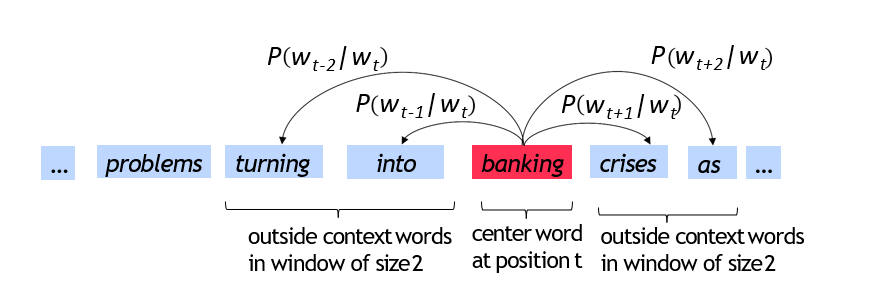
\includegraphics[width=\linewidth,keepaspectratio]{bert10}
\end{center}	

{\tiny (Ref: CS224n: Natural Language Processing with Deep Learning - Christopher Manning)}

\end{frame}

%%%%%%%%%%%%%%%%%%%%%%%%%%%%%%%%%%%%%%%%%%%%%%%%%%%%%%%%%%%
\begin{frame}[fragile]\frametitle{Word2Vec objective function}


\begin{center}
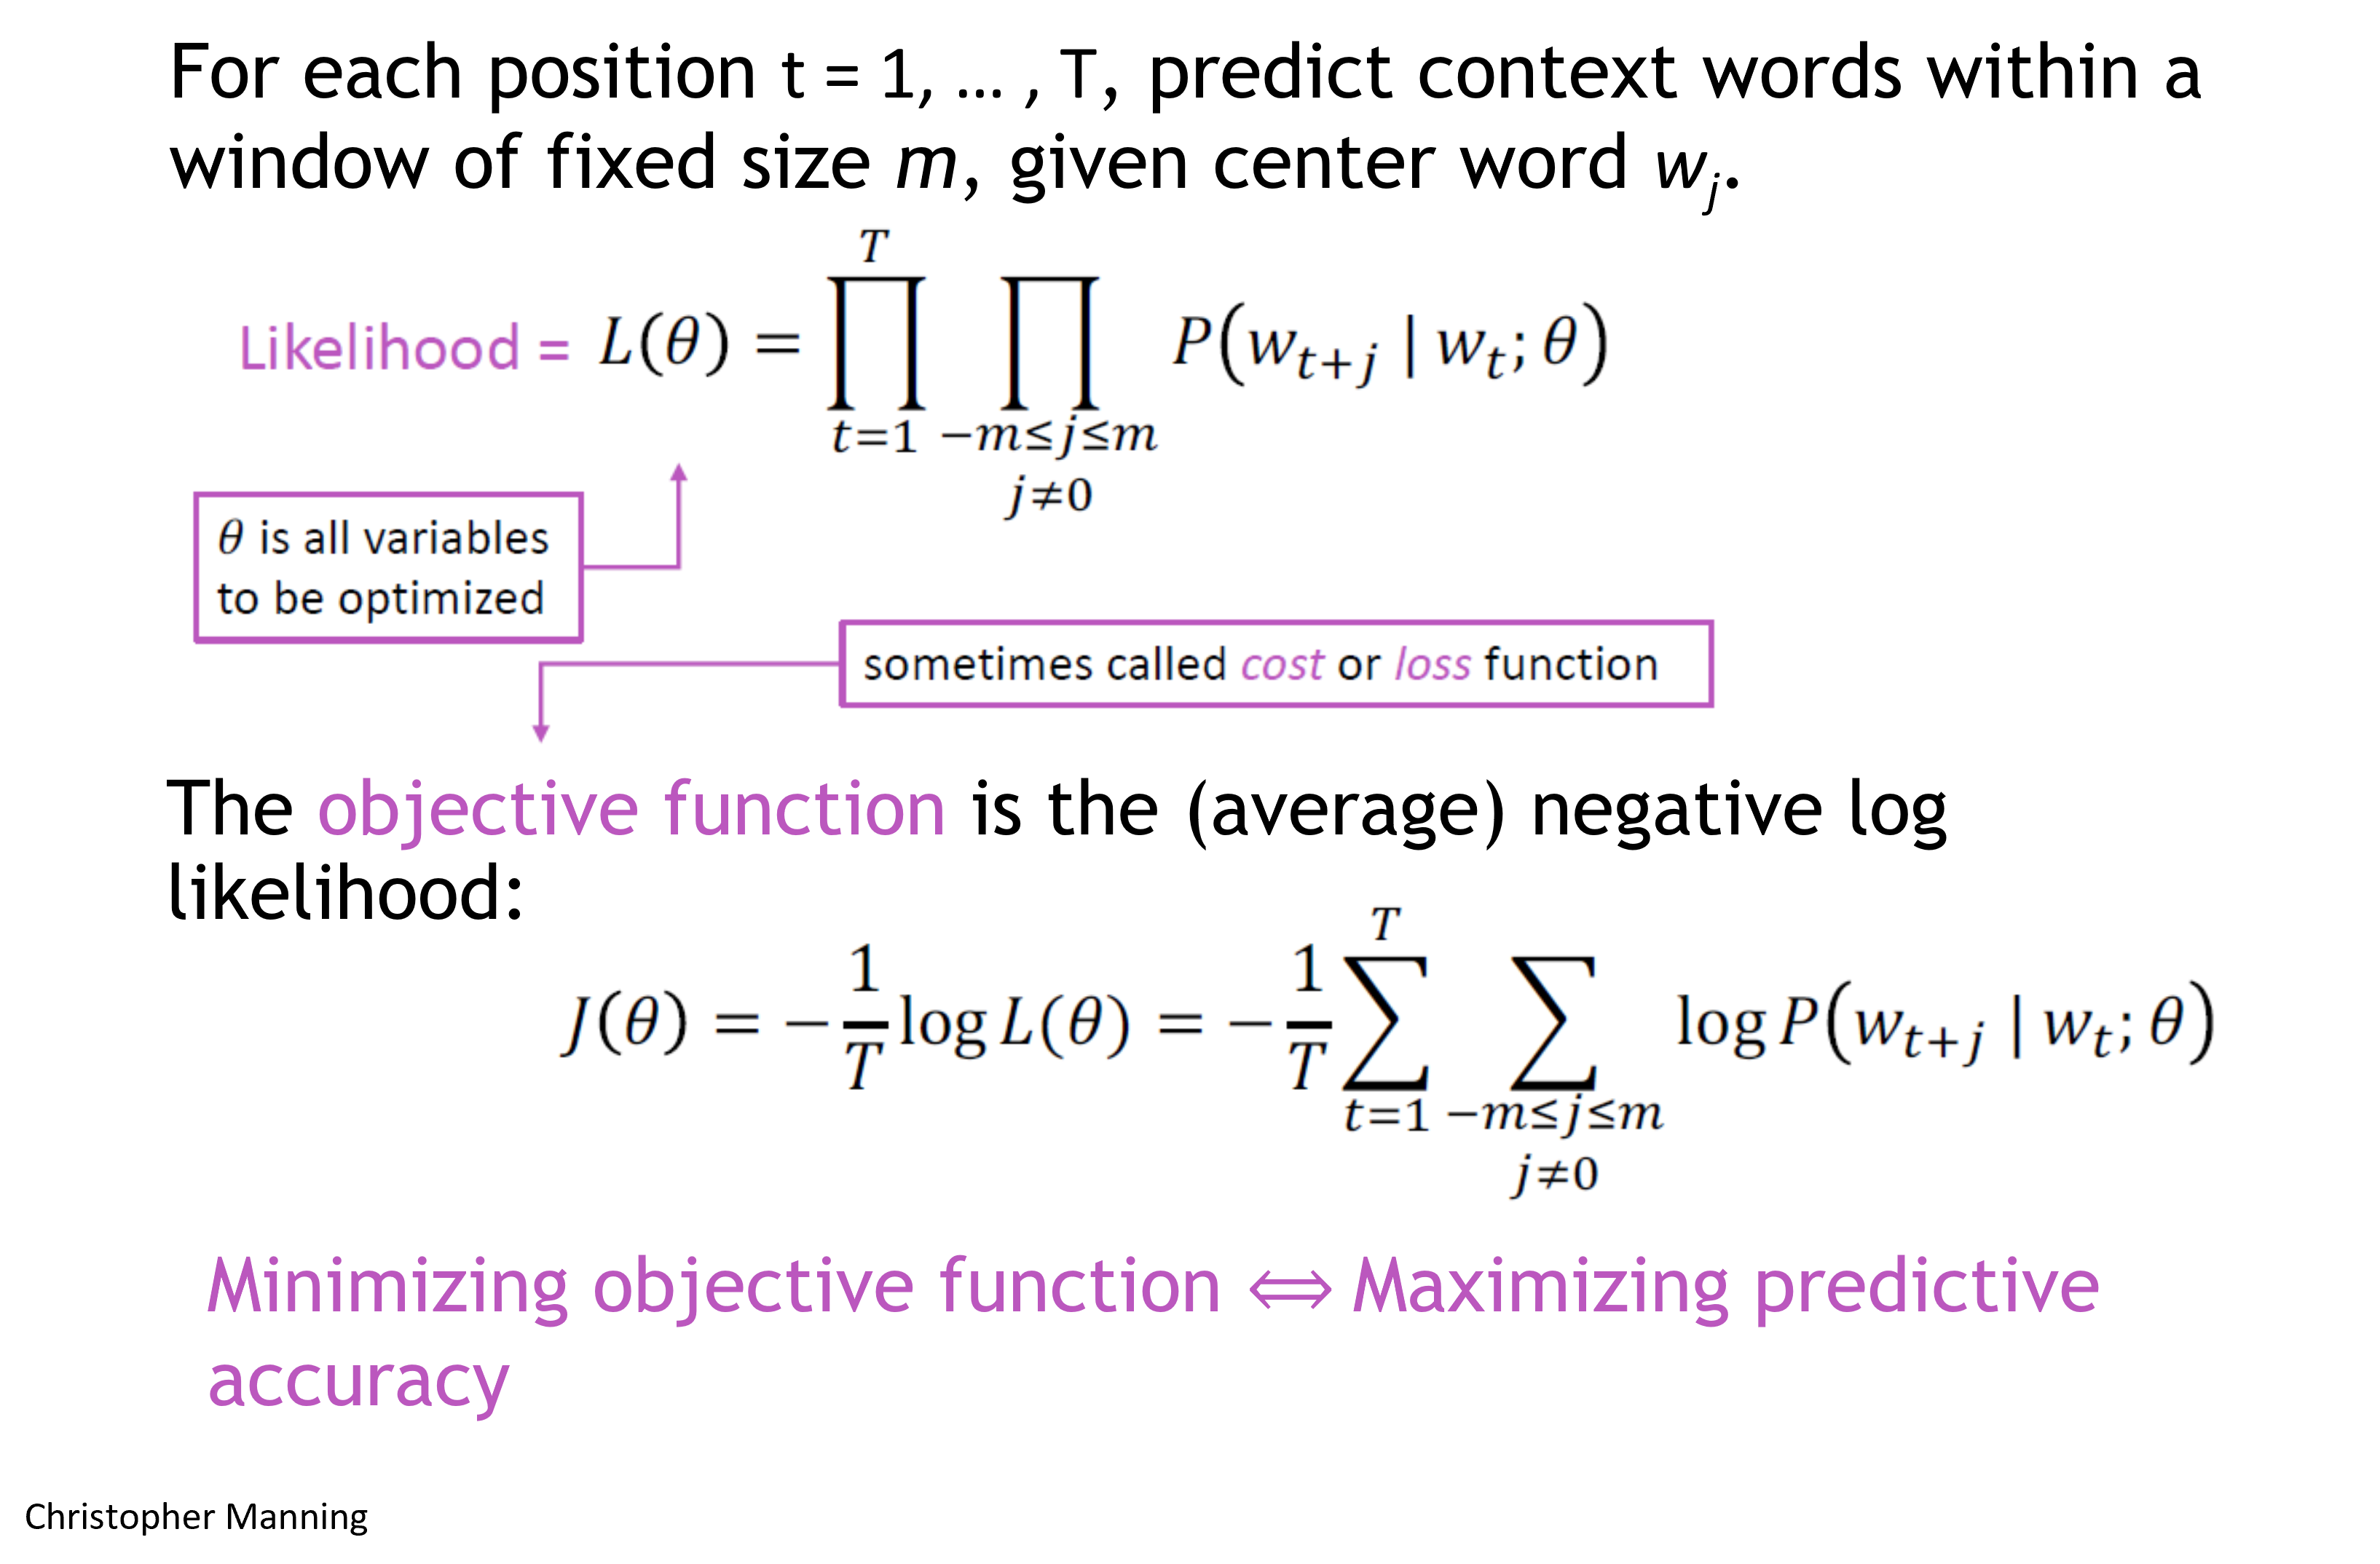
\includegraphics[width=0.9\linewidth,keepaspectratio]{bert11}
\end{center}	

{\tiny (Ref: CS224n: Natural Language Processing with Deep Learning - Christopher Manning)}

\end{frame}

%%%%%%%%%%%%%%%%%%%%%%%%%%%%%%%%%%%%%%%%%%%%%%%%%%%%%%%%%%%
\begin{frame}[fragile]\frametitle{Word2Vec objective function}


\begin{center}
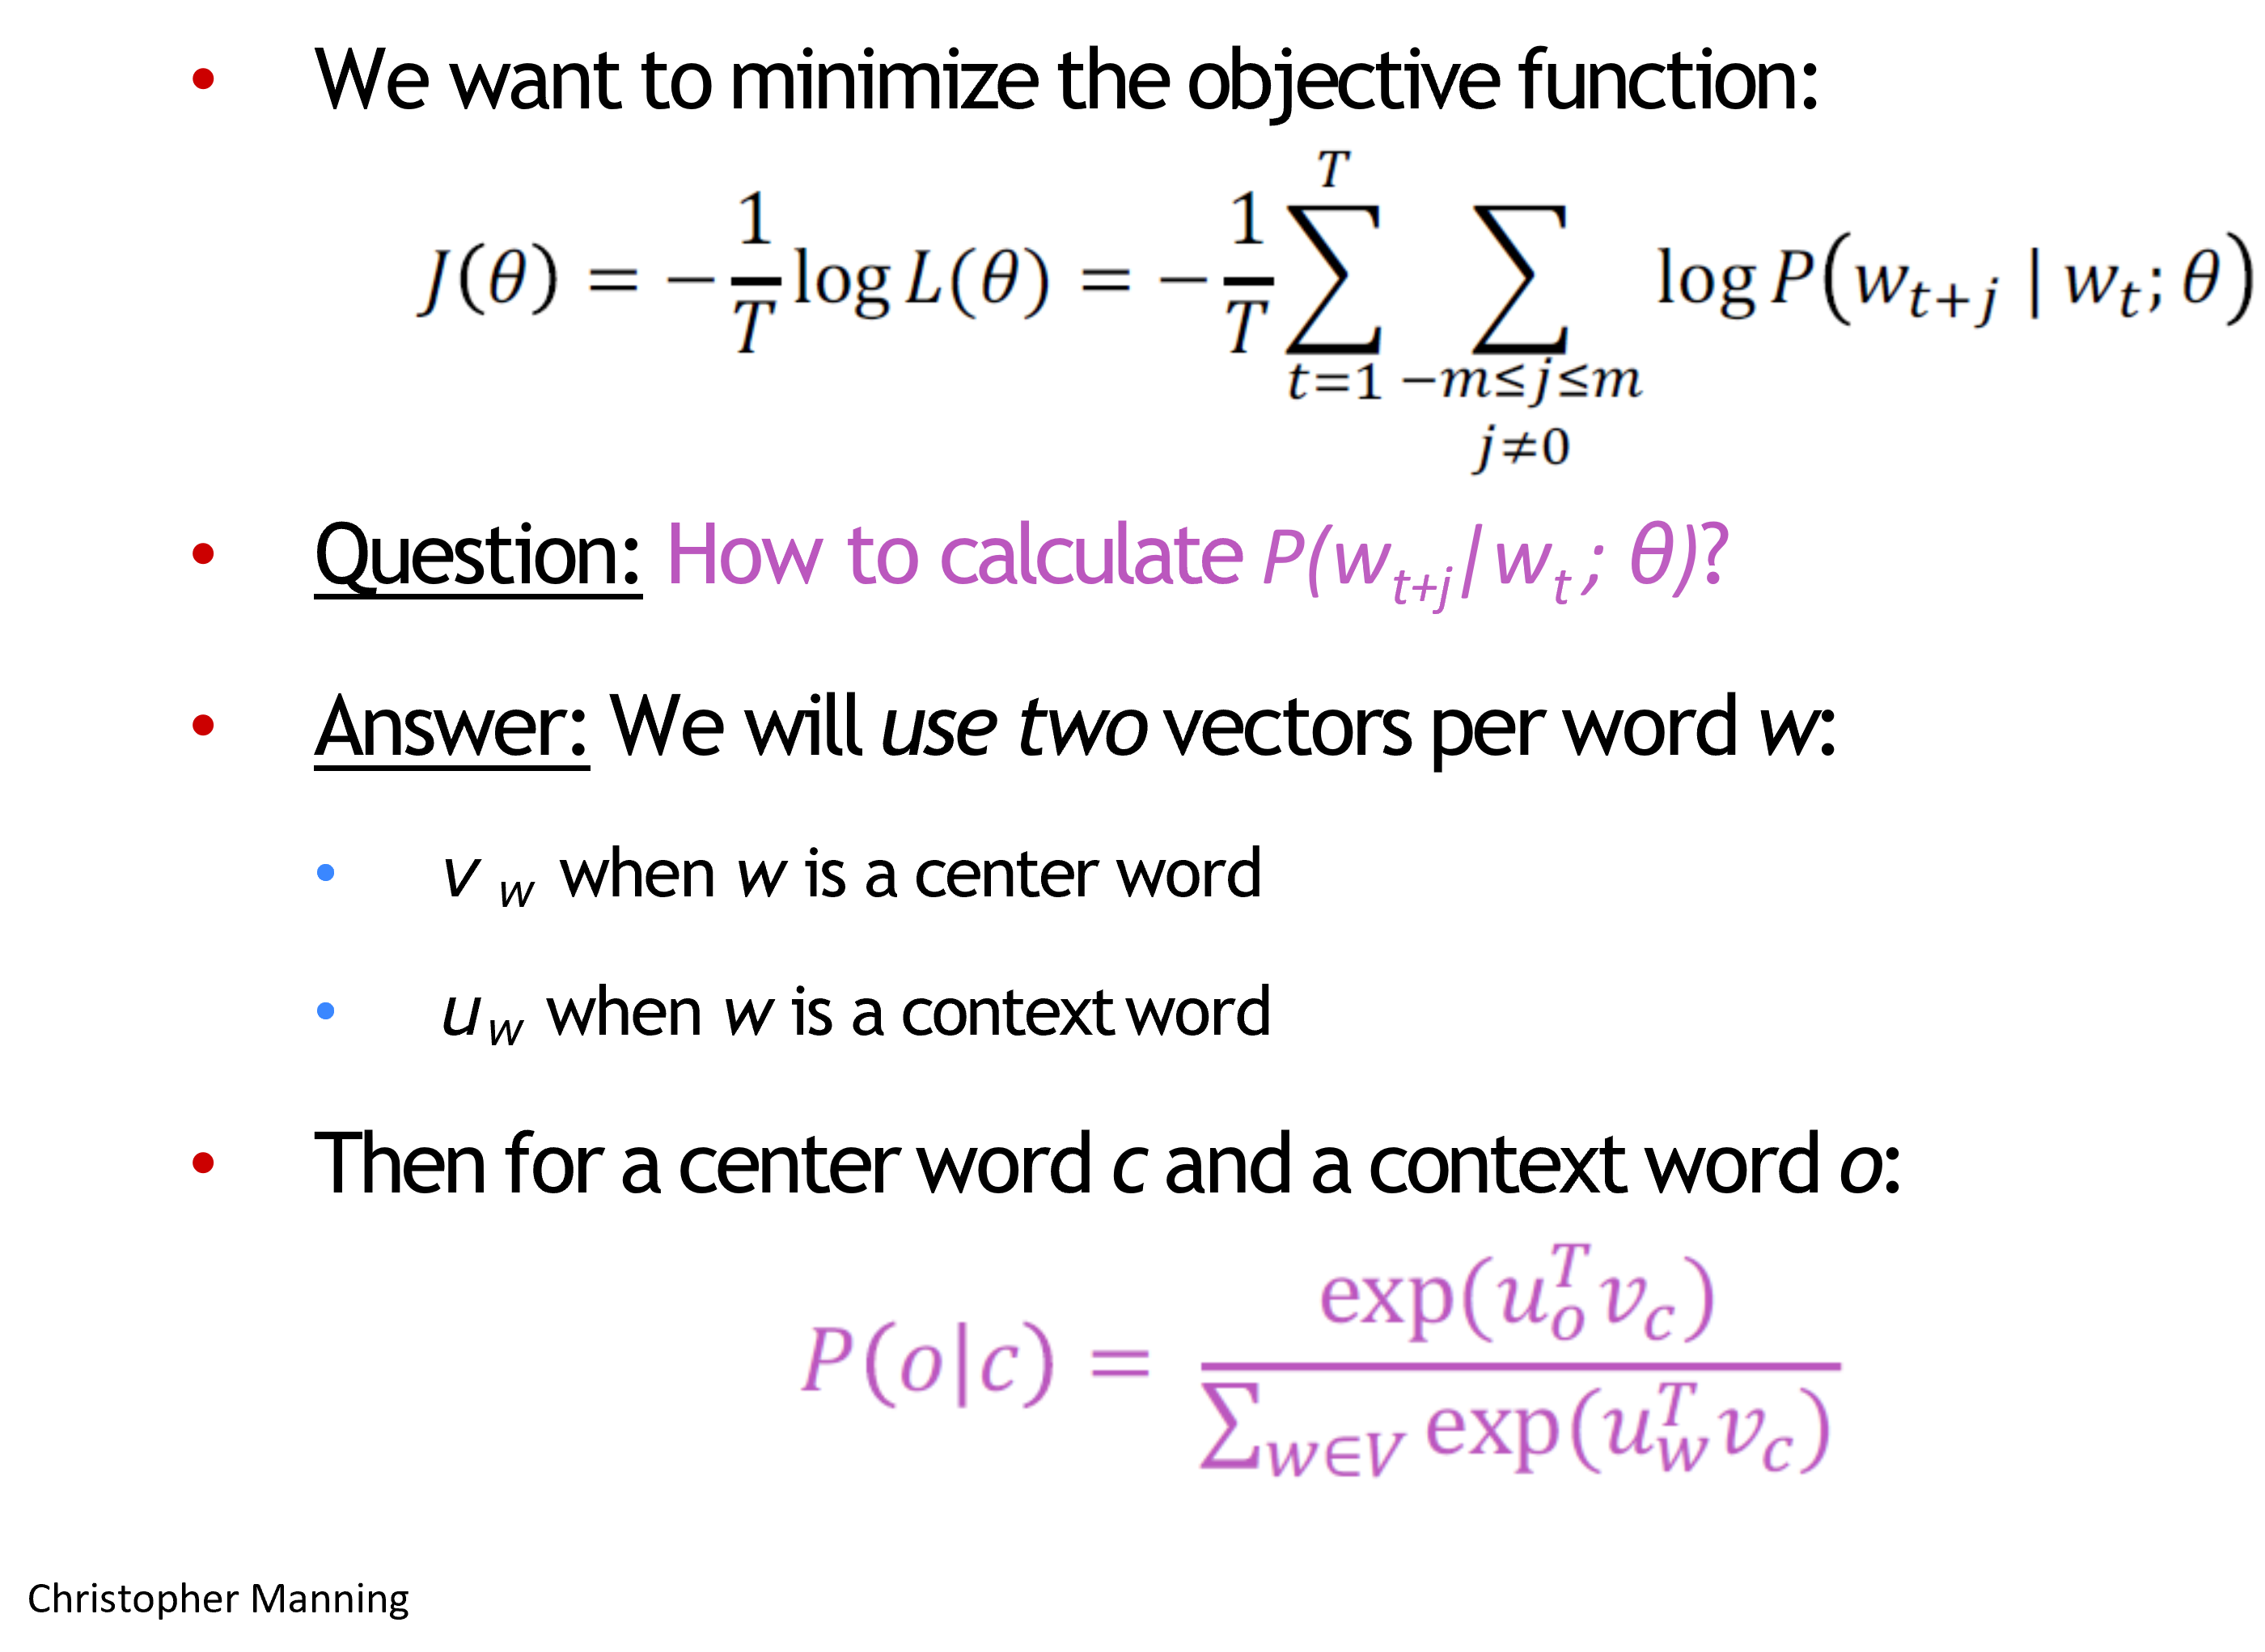
\includegraphics[width=0.9\linewidth,keepaspectratio]{bert12}
\end{center}	

{\tiny (Ref: CS224n: Natural Language Processing with Deep Learning - Christopher Manning)}

\end{frame}

%%%%%%%%%%%%%%%%%%%%%%%%%%%%%%%%%%%%%%%%%%%%%%%%%%%%%%%%%%%
\begin{frame}[fragile]\frametitle{Word2Vec prediction function}


\begin{center}
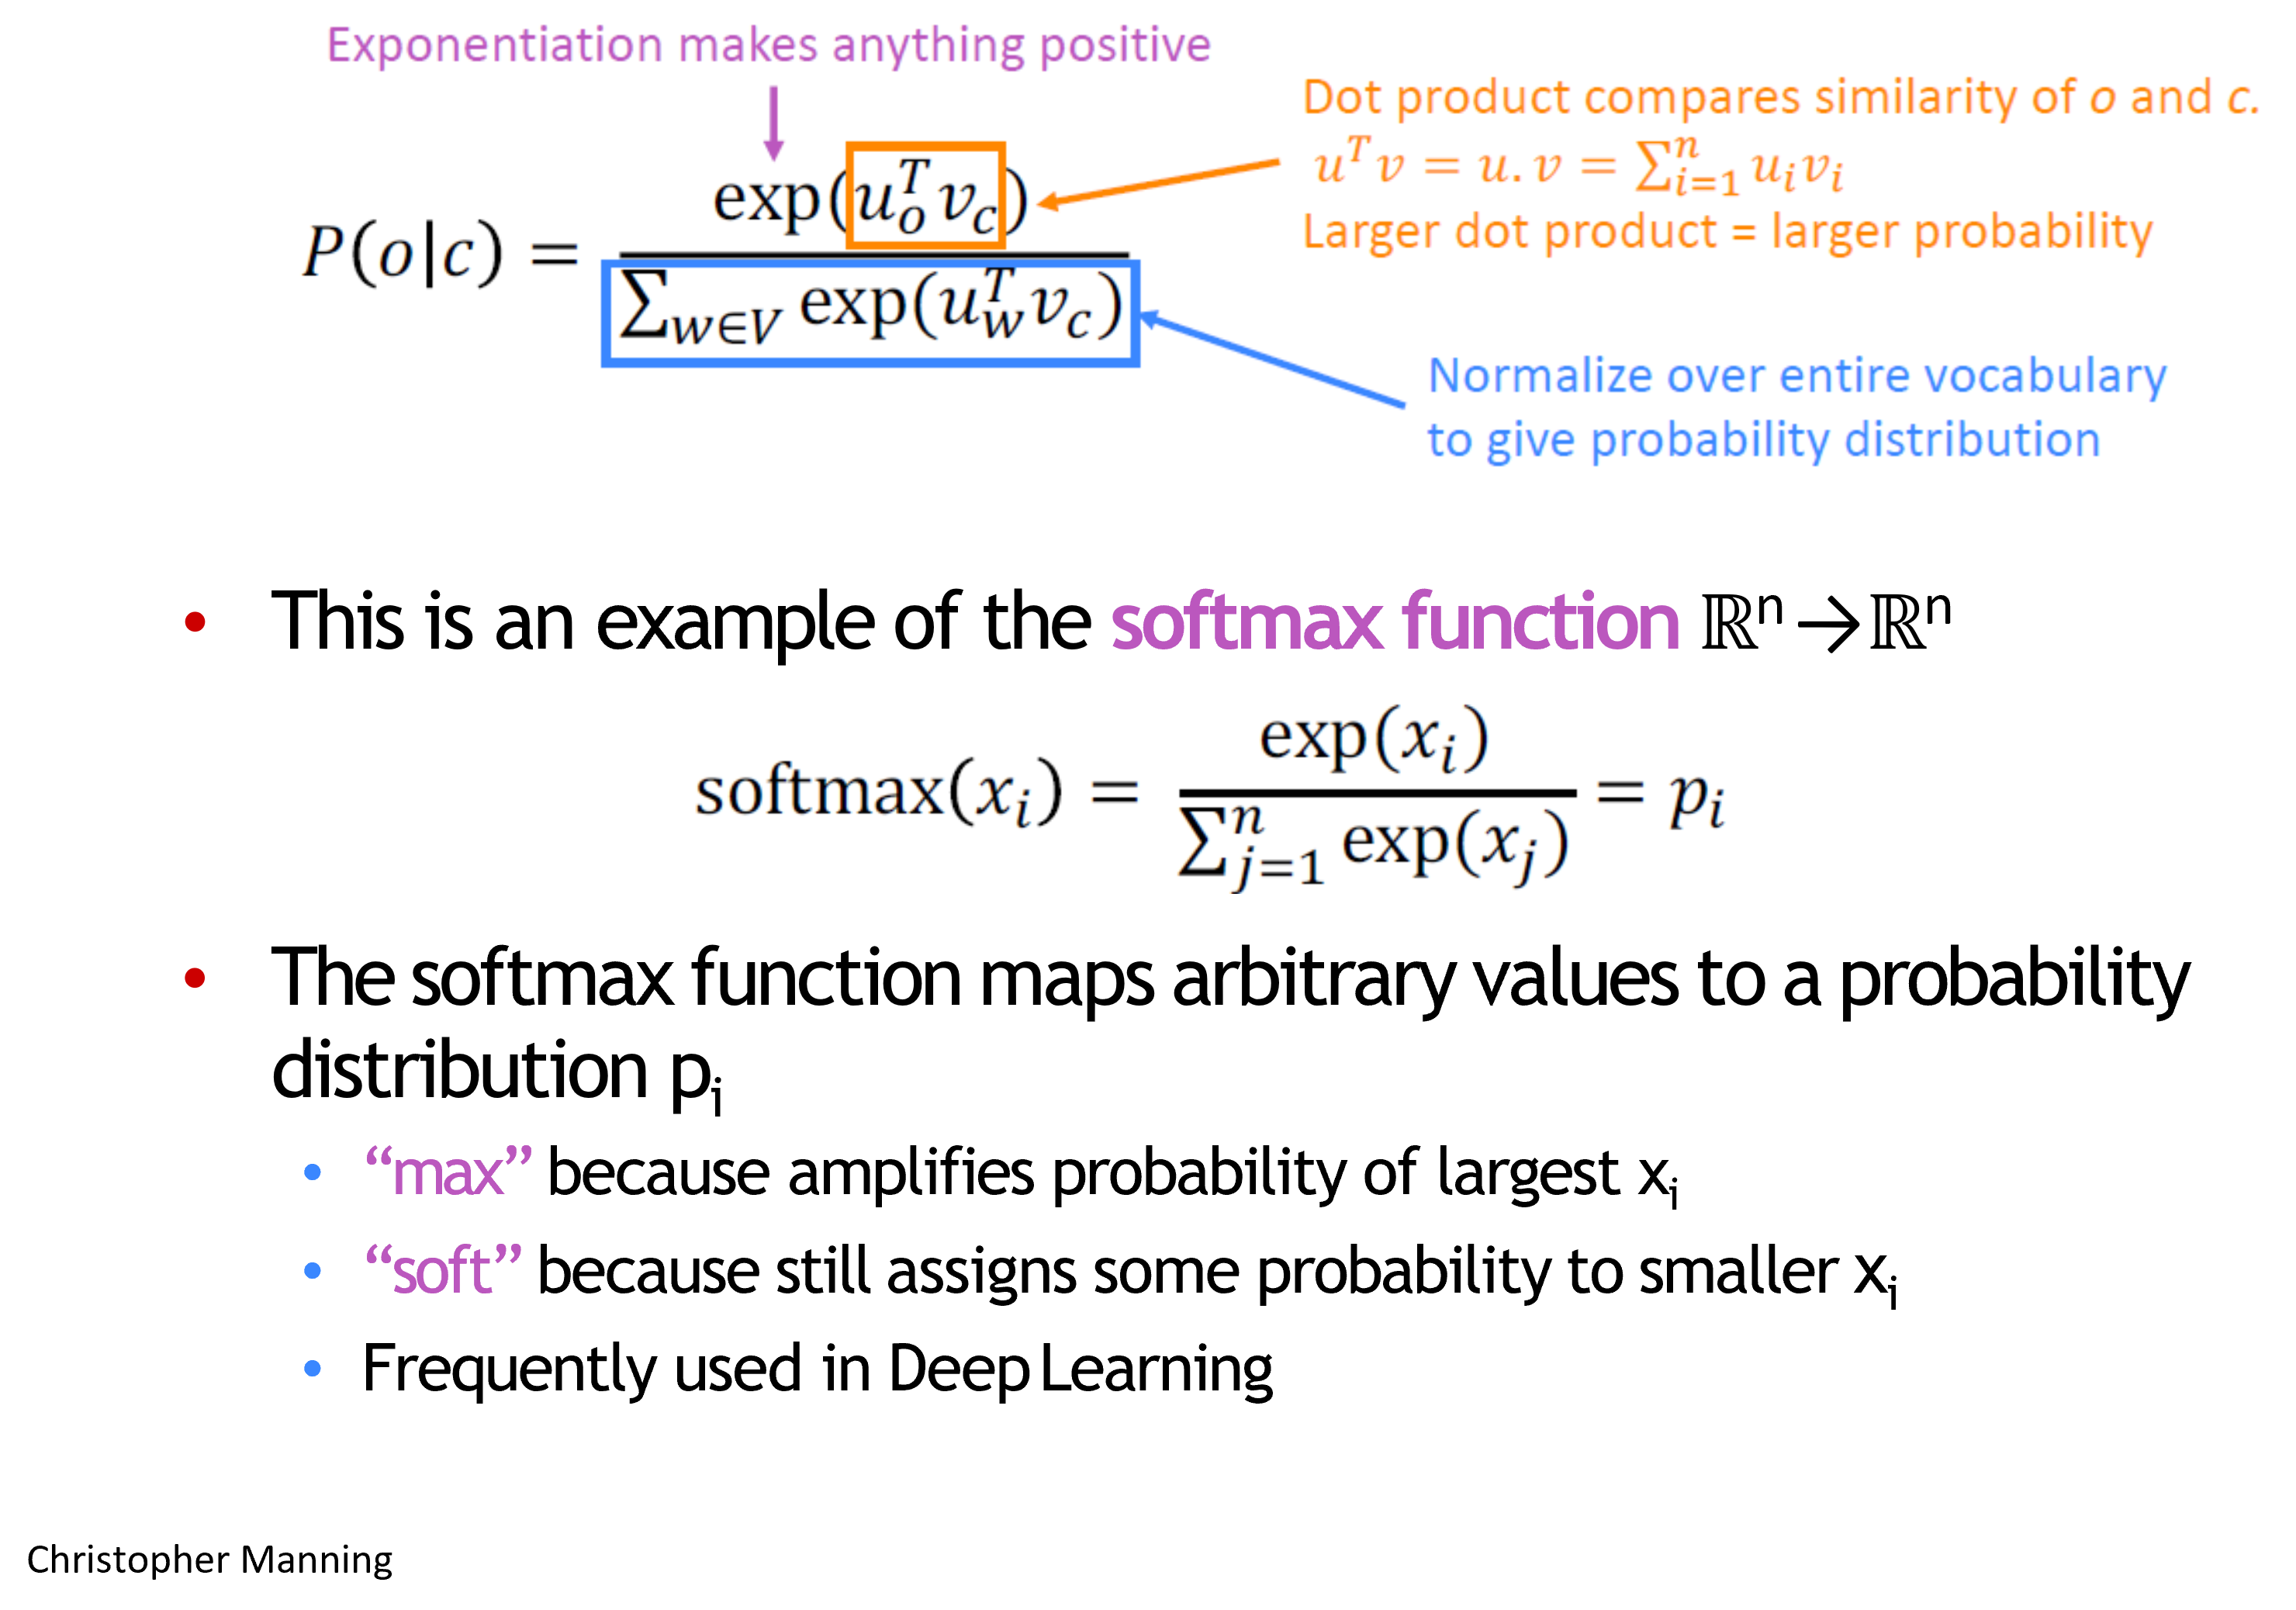
\includegraphics[width=0.9\linewidth,keepaspectratio]{bert13}
\end{center}	

{\tiny (Ref: CS224n: Natural Language Processing with Deep Learning - Christopher Manning)}

\end{frame}

%%%%%%%%%%%%%%%%%%%%%%%%%%%%%%%%%%%%%%%%%%%%%%%%%%%%%%%%%%%%%%%%%%%%%%%%%%%%%%%%%%
\begin{frame}[fragile]\frametitle{}
\begin{center}
{\Large Sequence Recurrence Models \\ \small RNNs and LSTMs}
\end{center}
\end{frame}


%%%%%%%%%%%%%%%%%%%%%%%%%%%%%%%%%%%%%%%%%%%%%%%%%%%%%%%%%%%
\begin{frame}[fragile]\frametitle{Sequence-to-Sequence (seq2seq)}

\begin{center}
See any issues with this traditional seq2seq paradigm?
\end{center}	

\end{frame}


%%%%%%%%%%%%%%%%%%%%%%%%%%%%%%%%%%%%%%%%%%%%%%%%%%%%%%%%%%%
\begin{frame}[fragile]\frametitle{Sequence-to-Sequence (seq2seq)}

\begin{center}
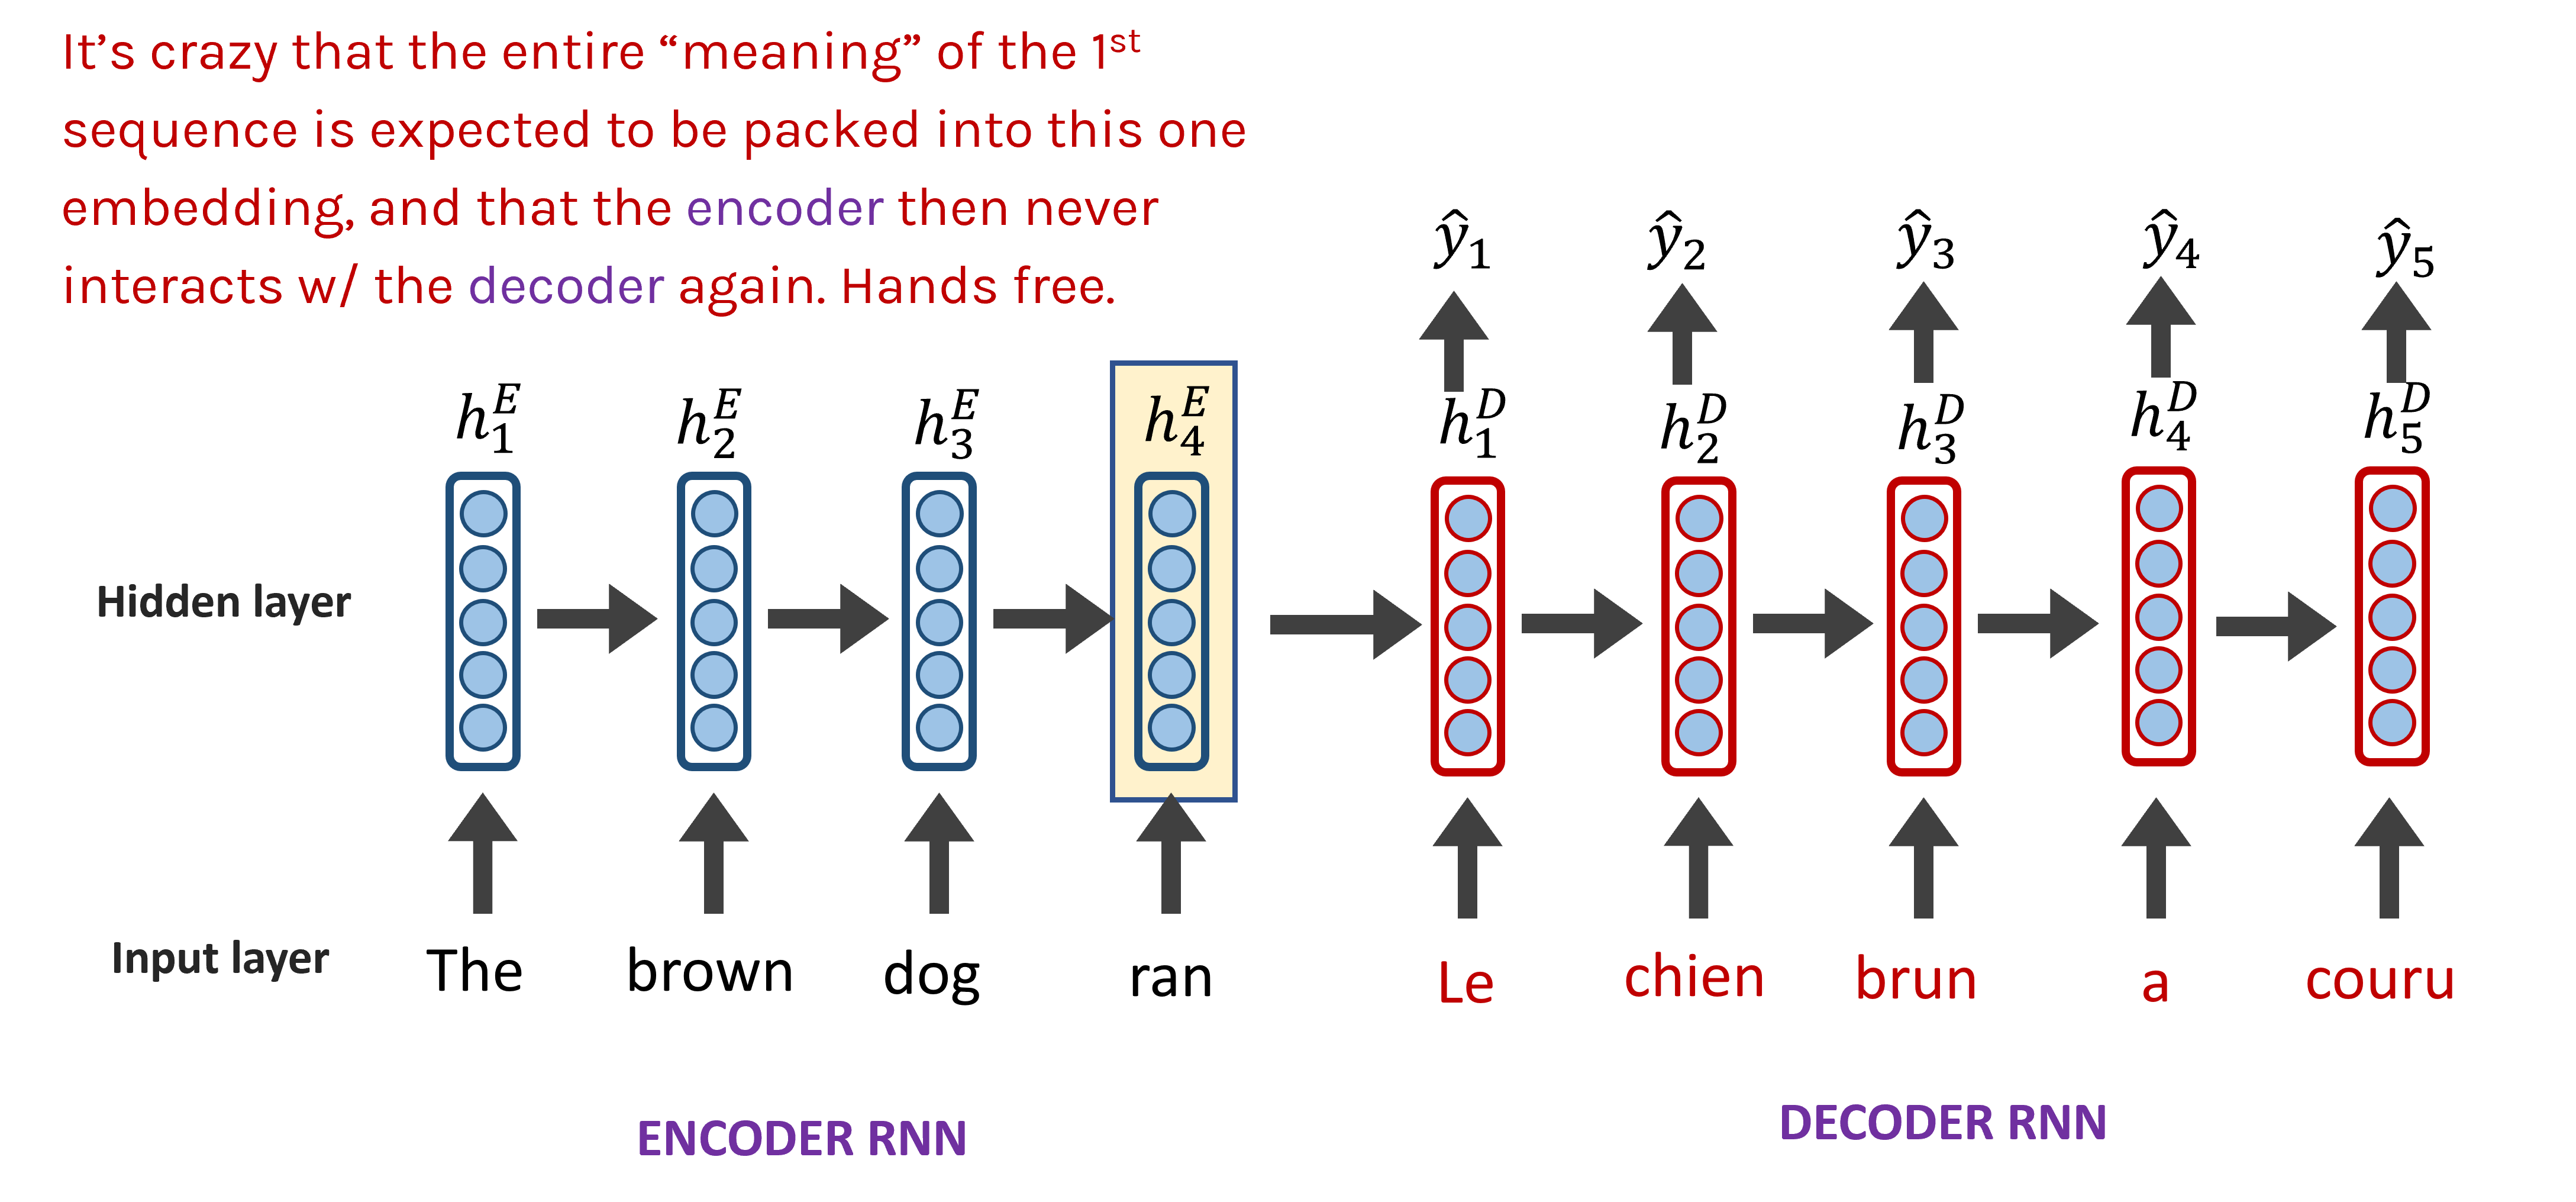
\includegraphics[width=\linewidth,keepaspectratio]{bert14}
\end{center}	

\end{frame}

%%%%%%%%%%%%%%%%%%%%%%%%%%%%%%%%%%%%%%%%%%%%%%%%%%%%%%%%%%%
\begin{frame}[fragile]\frametitle{Sequence-to-Sequence (seq2seq)}

\begin{center}
Instead, what if the decoder, at each step, pays {\bf attention} to a distribution of all of the encoder’s hidden states?
\end{center}	

\end{frame}

%%%%%%%%%%%%%%%%%%%%%%%%%%%%%%%%%%%%%%%%%%%%%%%%%%%%%%%%%%%
\begin{frame}[fragile]\frametitle{seq2seq + Attention}

Q: How do we determine how much to pay attention to each of the encoder’s hidden layers? 

\begin{center}
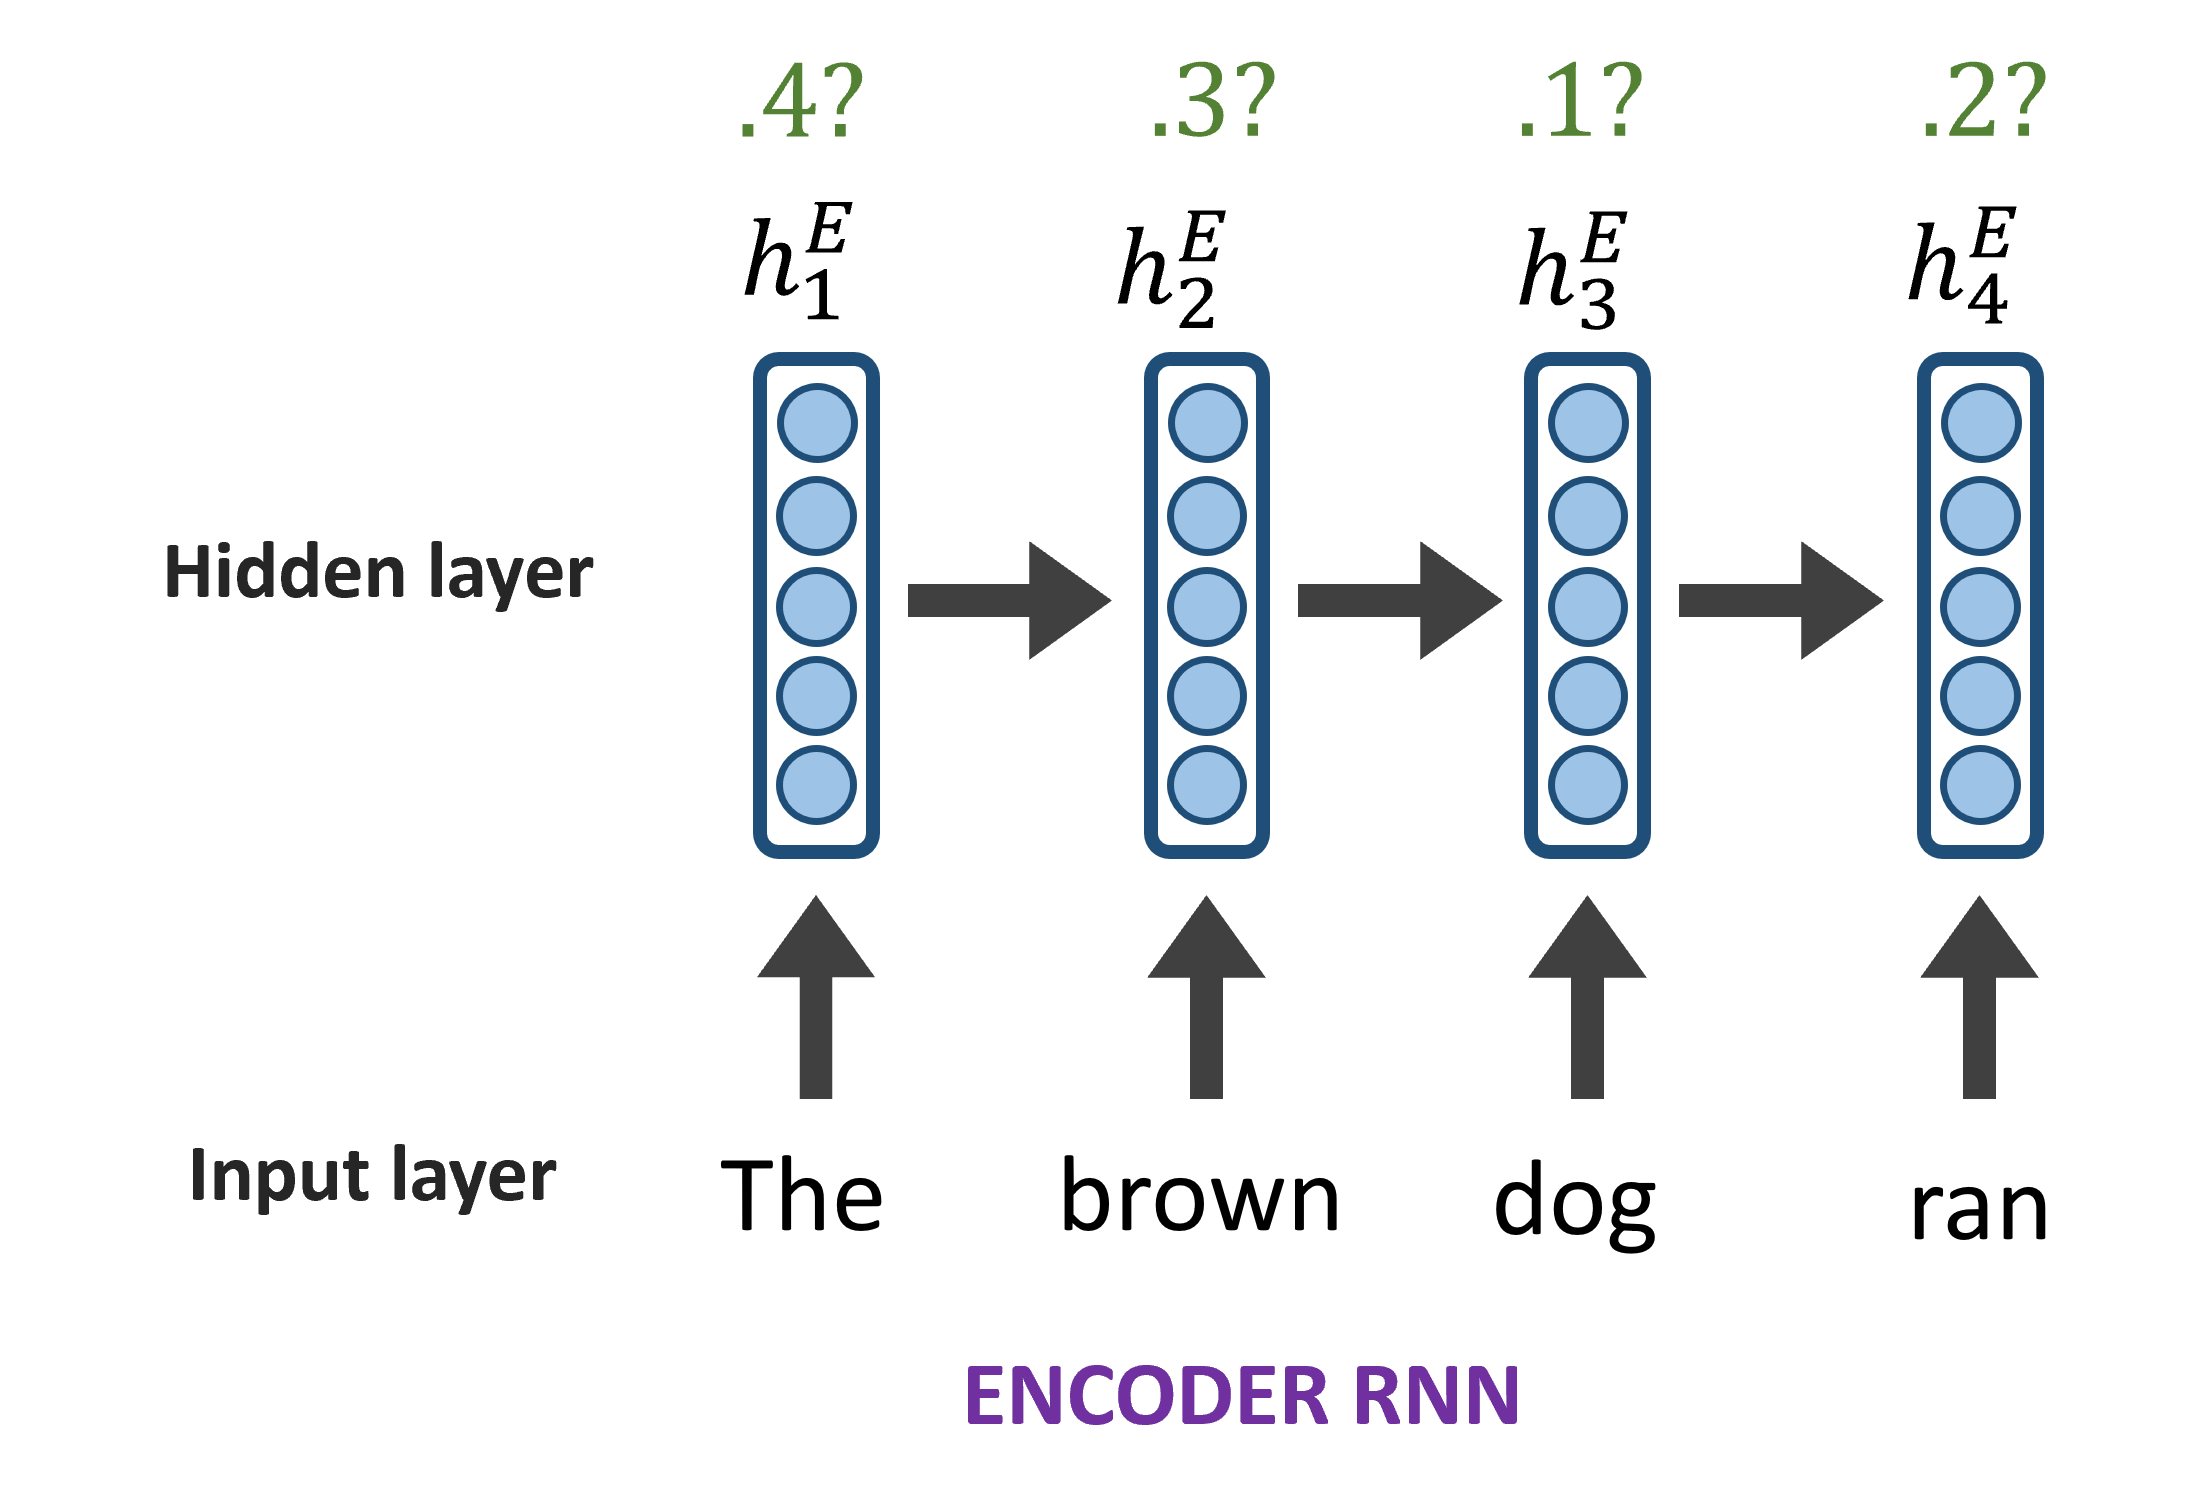
\includegraphics[width=0.8\linewidth,keepaspectratio]{bert15}
\end{center}	

\end{frame}


%%%%%%%%%%%%%%%%%%%%%%%%%%%%%%%%%%%%%%%%%%%%%%%%%%%%%%%%%%%
\begin{frame}[fragile]\frametitle{seq2seq + Attention}

Q: How do we determine how much to pay attention to each of the encoder’s hidden layers? 

A: Let’s base it on our decoder’s previous hidden state (our latest representation of meaning) and all of the encoder’s hidden layers!


\begin{center}
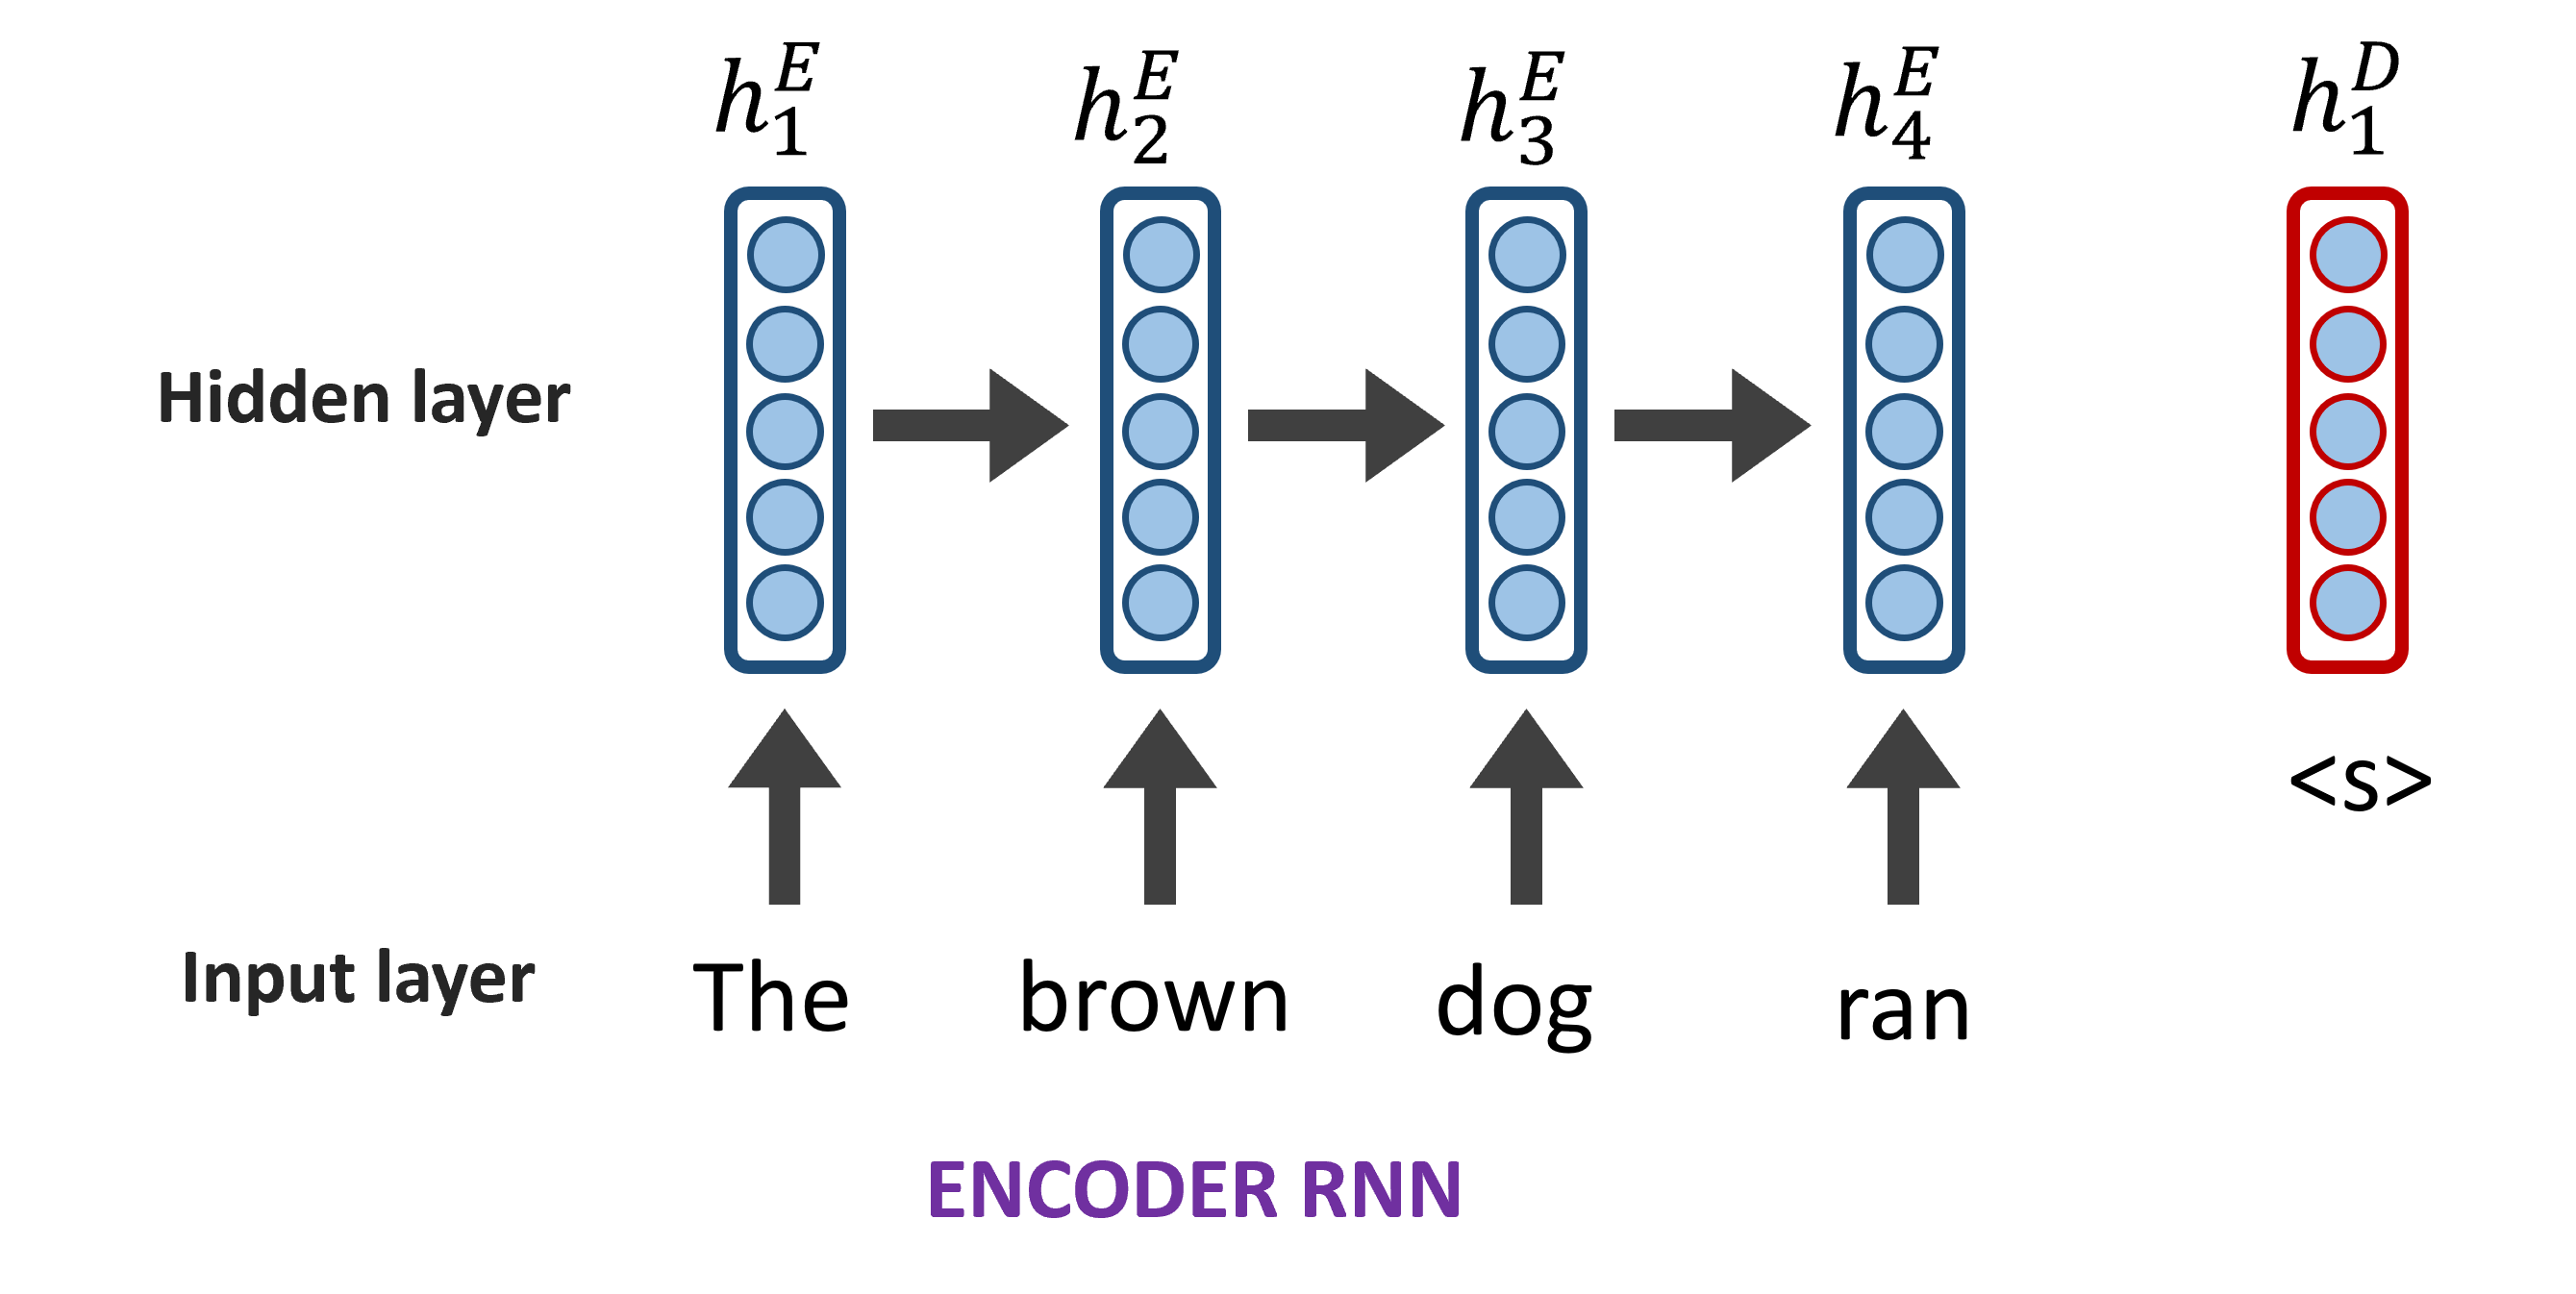
\includegraphics[width=0.8\linewidth,keepaspectratio]{bert16}
\end{center}	

\end{frame}

%%%%%%%%%%%%%%%%%%%%%%%%%%%%%%%%%%%%%%%%%%%%%%%%%%%%%%%%%%%
\begin{frame}[fragile]\frametitle{seq2seq + Attention}

Q: How do we determine how much to pay attention to each of the encoder’s hidden layers? 

A: Let’s base it on our decoder’s previous hidden state (our latest representation of meaning) and all of the encoder’s hidden layers!


\begin{center}
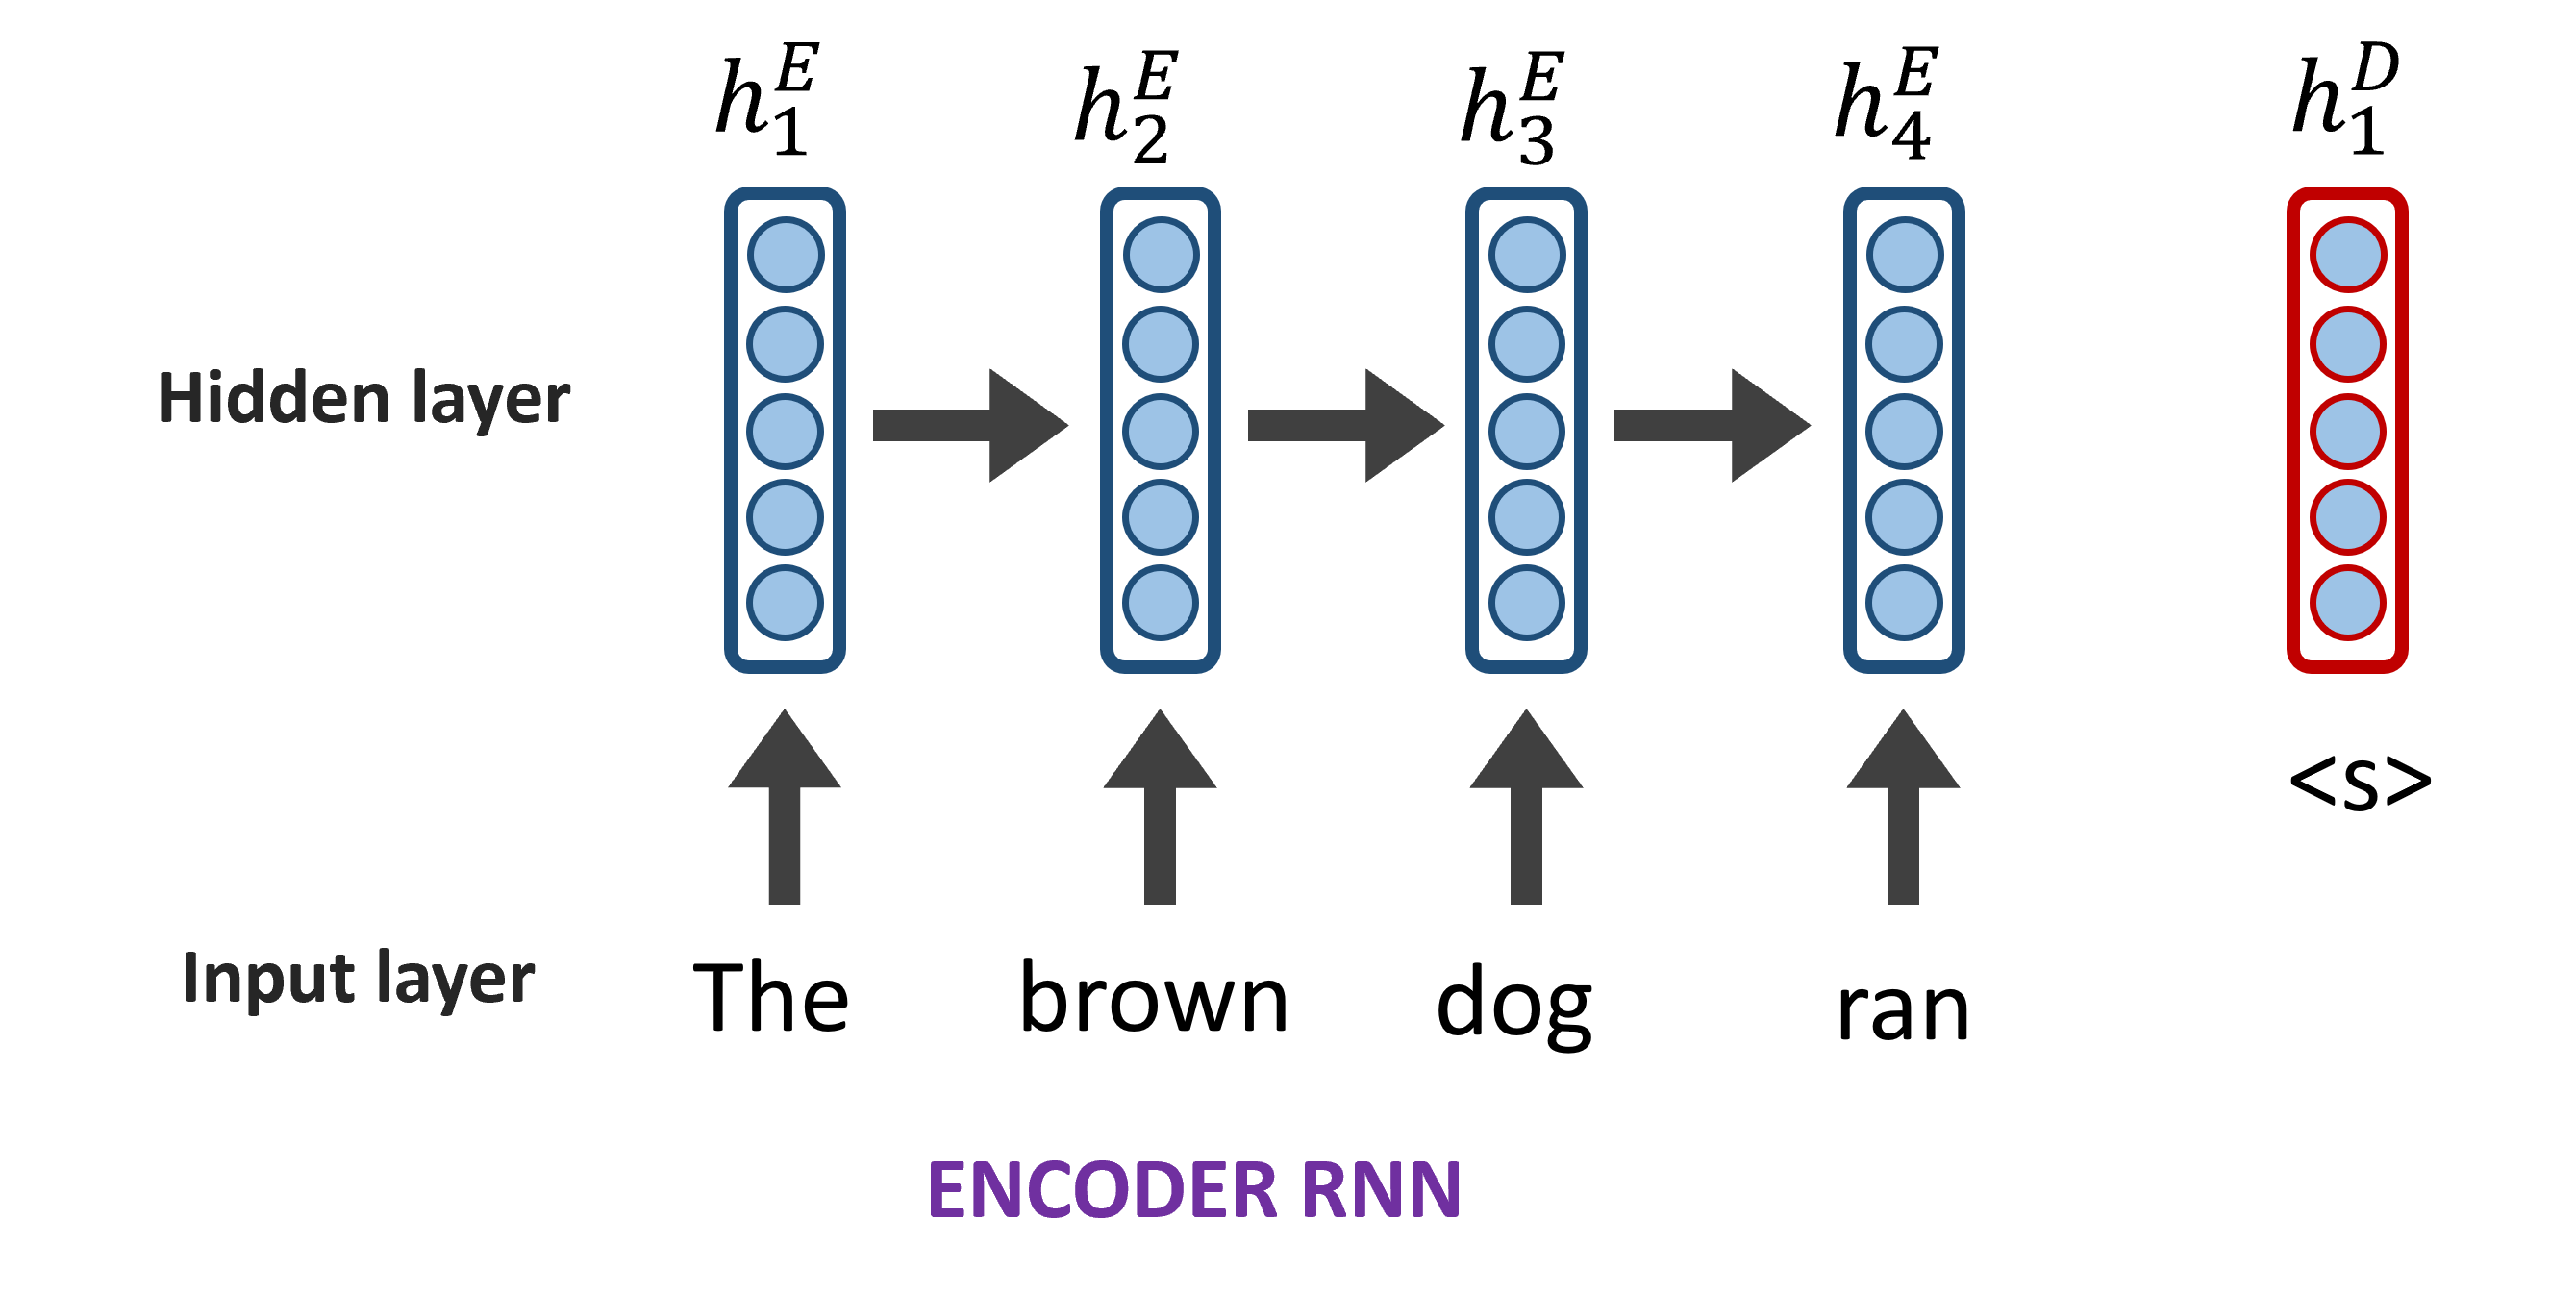
\includegraphics[width=0.8\linewidth,keepaspectratio]{bert17}
\end{center}	

\end{frame}

%%%%%%%%%%%%%%%%%%%%%%%%%%%%%%%%%%%%%%%%%%%%%%%%%%%%%%%%%%%
\begin{frame}[fragile]\frametitle{seq2seq + Attention}

Q: How do we determine how much to pay attention to each of the encoder’s hidden layers? 

A: Let’s base it on our decoder’s previous hidden state (our latest representation of meaning) and all of the encoder’s hidden layers! We want to measure similarity between decoder hidden state and encoder hidden stateS in some ways. 



\begin{center}
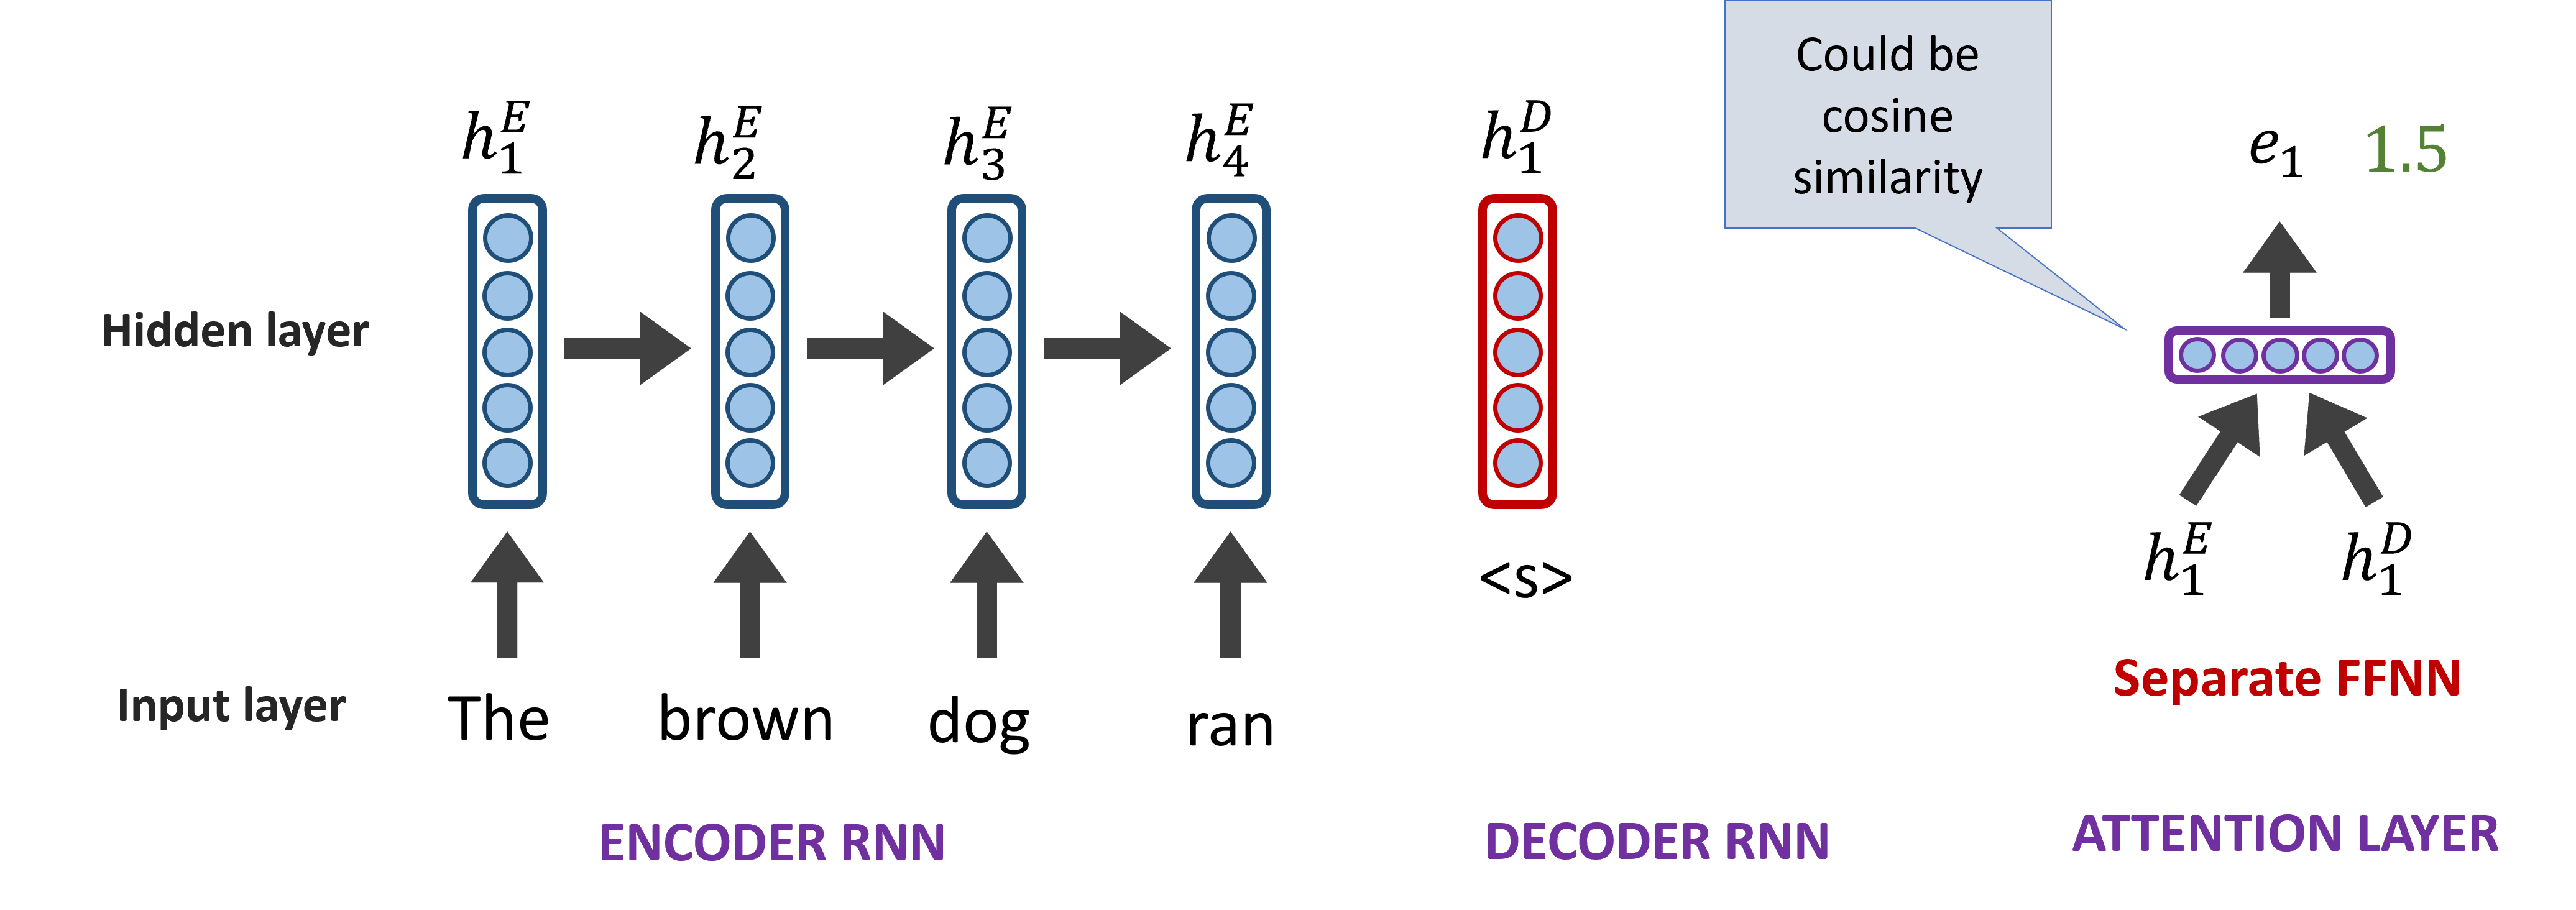
\includegraphics[width=0.8\linewidth,keepaspectratio]{bert18}
\end{center}	

\end{frame}

%%%%%%%%%%%%%%%%%%%%%%%%%%%%%%%%%%%%%%%%%%%%%%%%%%%%%%%%%%%
\begin{frame}[fragile]\frametitle{seq2seq + Attention}

Q: How do we determine how much to pay attention to each of the encoder’s hidden layers? 

A: Let’s base it on our decoder’s previous hidden state (our latest representation of meaning) and all of the encoder’s hidden layers! We want to measure similarity between decoder hidden state and encoder hidden stateS in some ways. 



\begin{center}
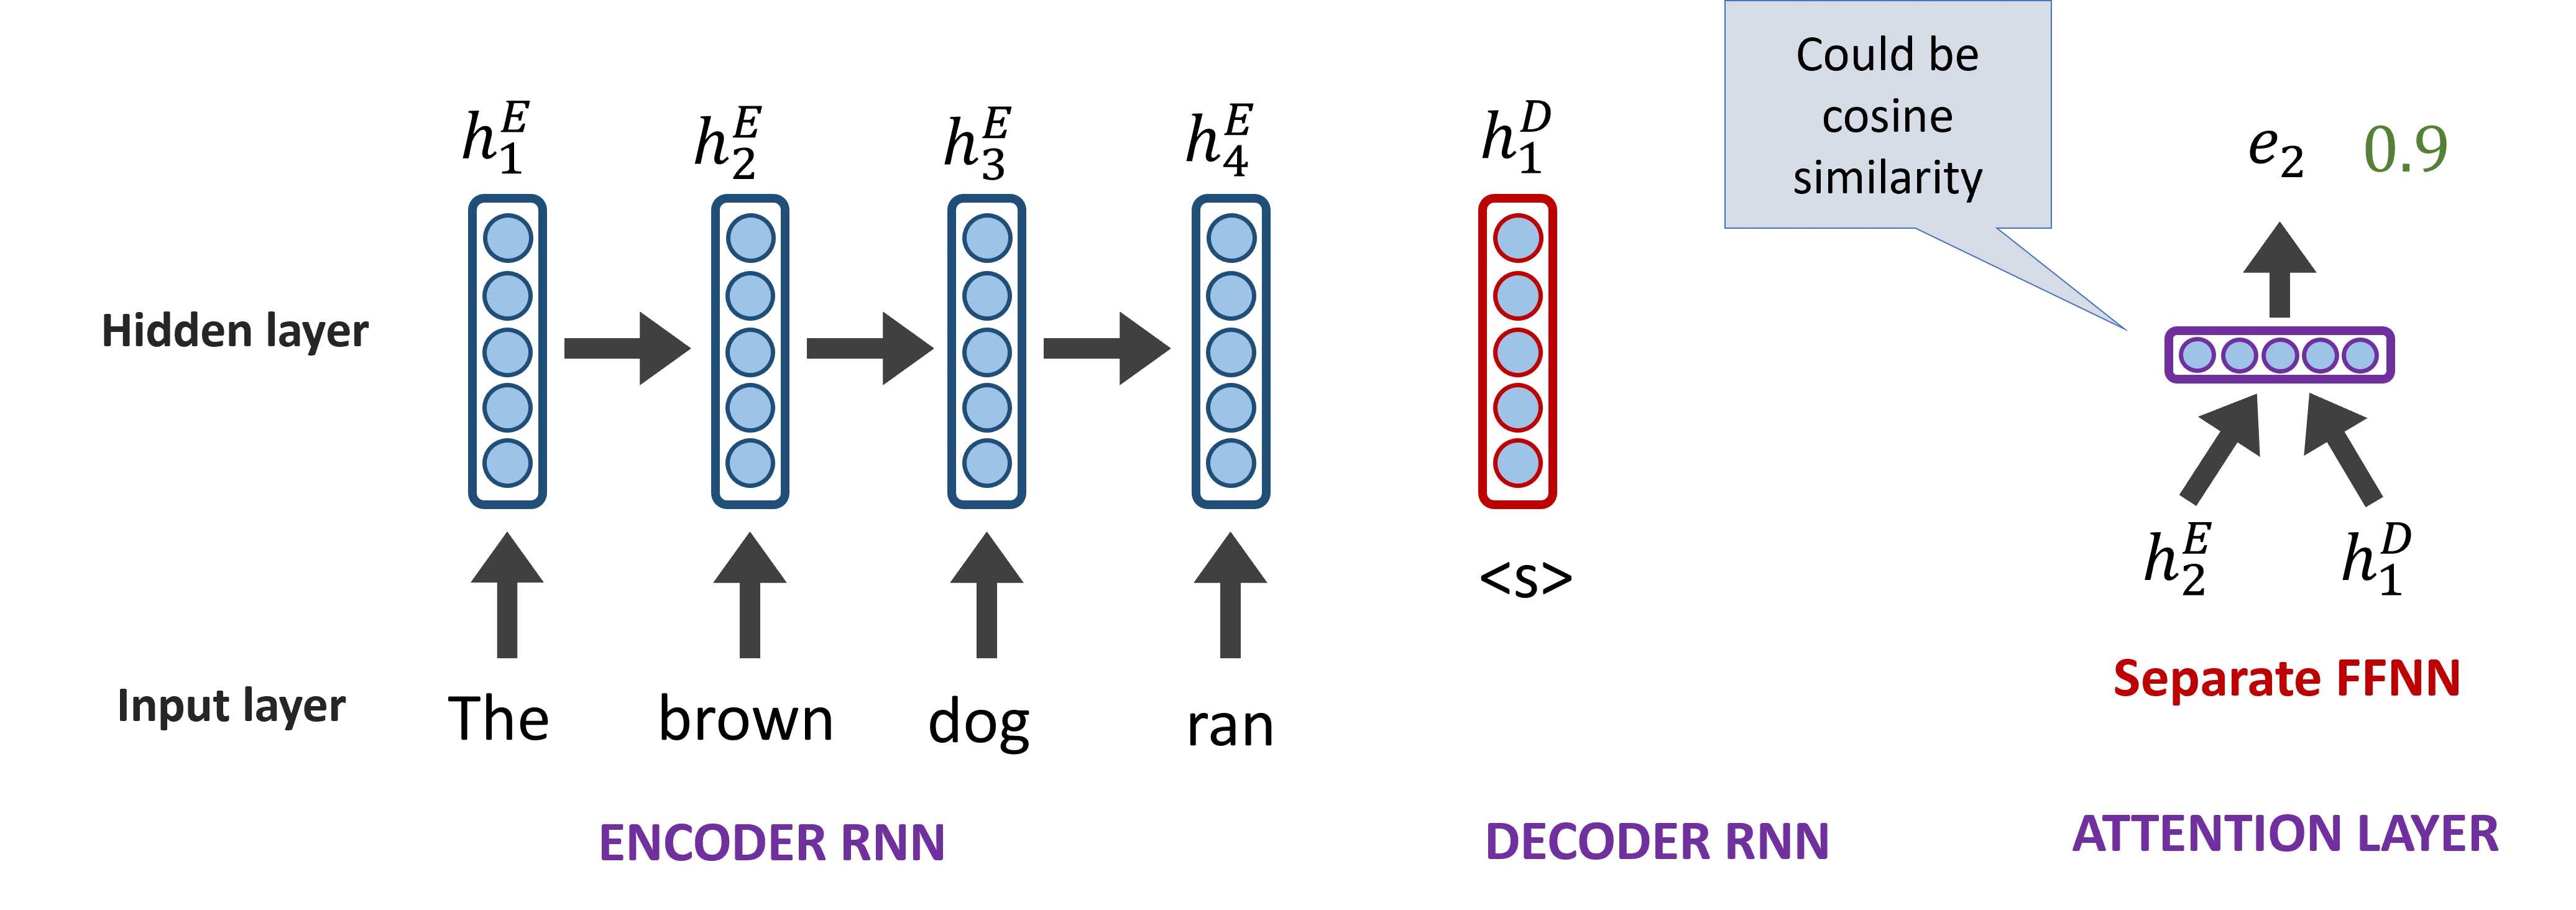
\includegraphics[width=0.8\linewidth,keepaspectratio]{bert19}
\end{center}	

\end{frame}

%%%%%%%%%%%%%%%%%%%%%%%%%%%%%%%%%%%%%%%%%%%%%%%%%%%%%%%%%%%
\begin{frame}[fragile]\frametitle{seq2seq + Attention}

Q: How do we determine how much to pay attention to each of the encoder’s hidden layers? 

A: Let’s base it on our decoder’s previous hidden state (our latest representation of meaning) and all of the encoder’s hidden layers! We want to measure similarity between decoder hidden state and encoder hidden stateS in some ways. 



\begin{center}
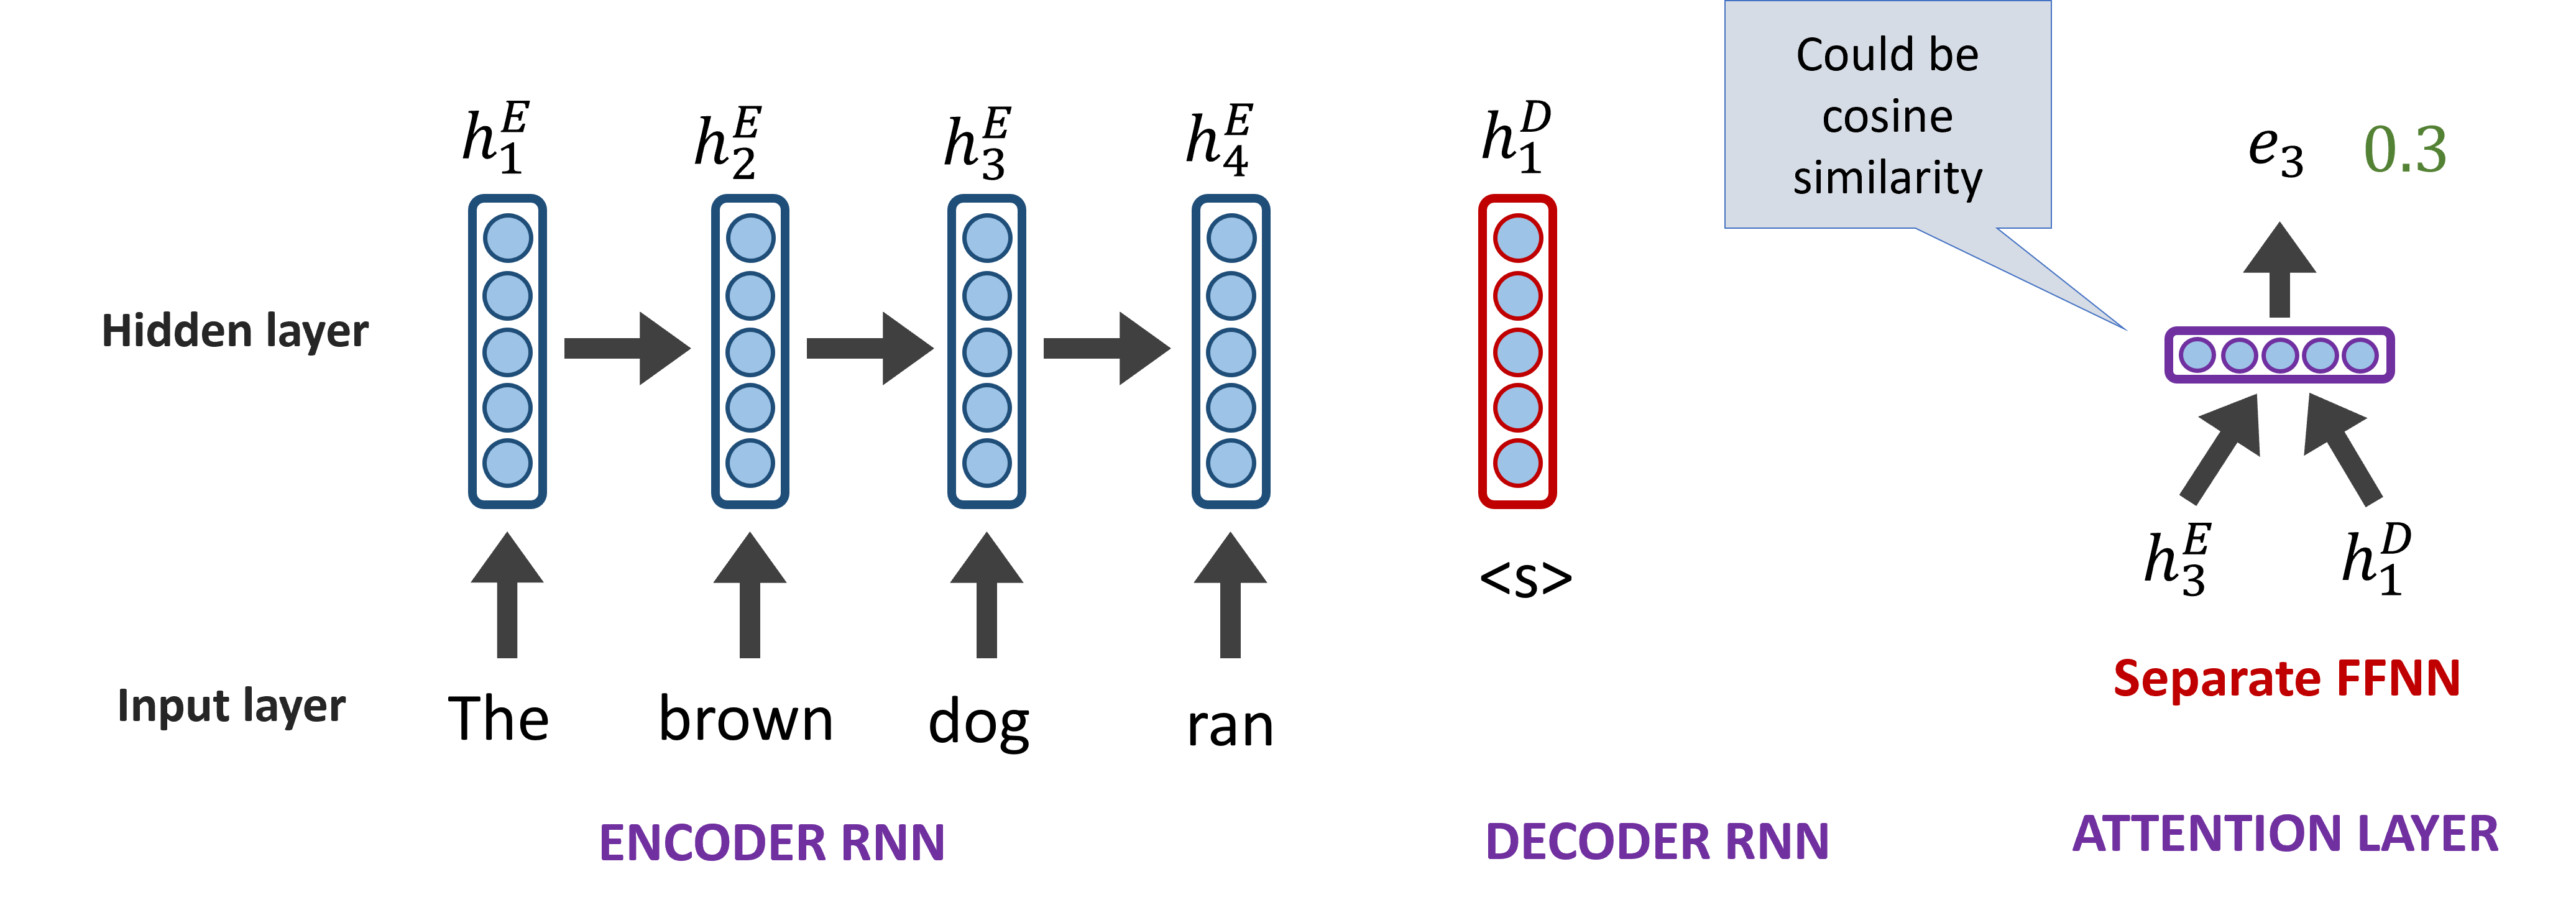
\includegraphics[width=0.8\linewidth,keepaspectratio]{bert20}
\end{center}	

\end{frame}

%%%%%%%%%%%%%%%%%%%%%%%%%%%%%%%%%%%%%%%%%%%%%%%%%%%%%%%%%%%
\begin{frame}[fragile]\frametitle{seq2seq + Attention}

Q: How do we determine how much to pay attention to each of the encoder’s hidden layers? 

A: Let’s base it on our decoder’s previous hidden state (our latest representation of meaning) and all of the encoder’s hidden layers! We want to measure similarity between decoder hidden state and encoder hidden stateS in some ways. 



\begin{center}
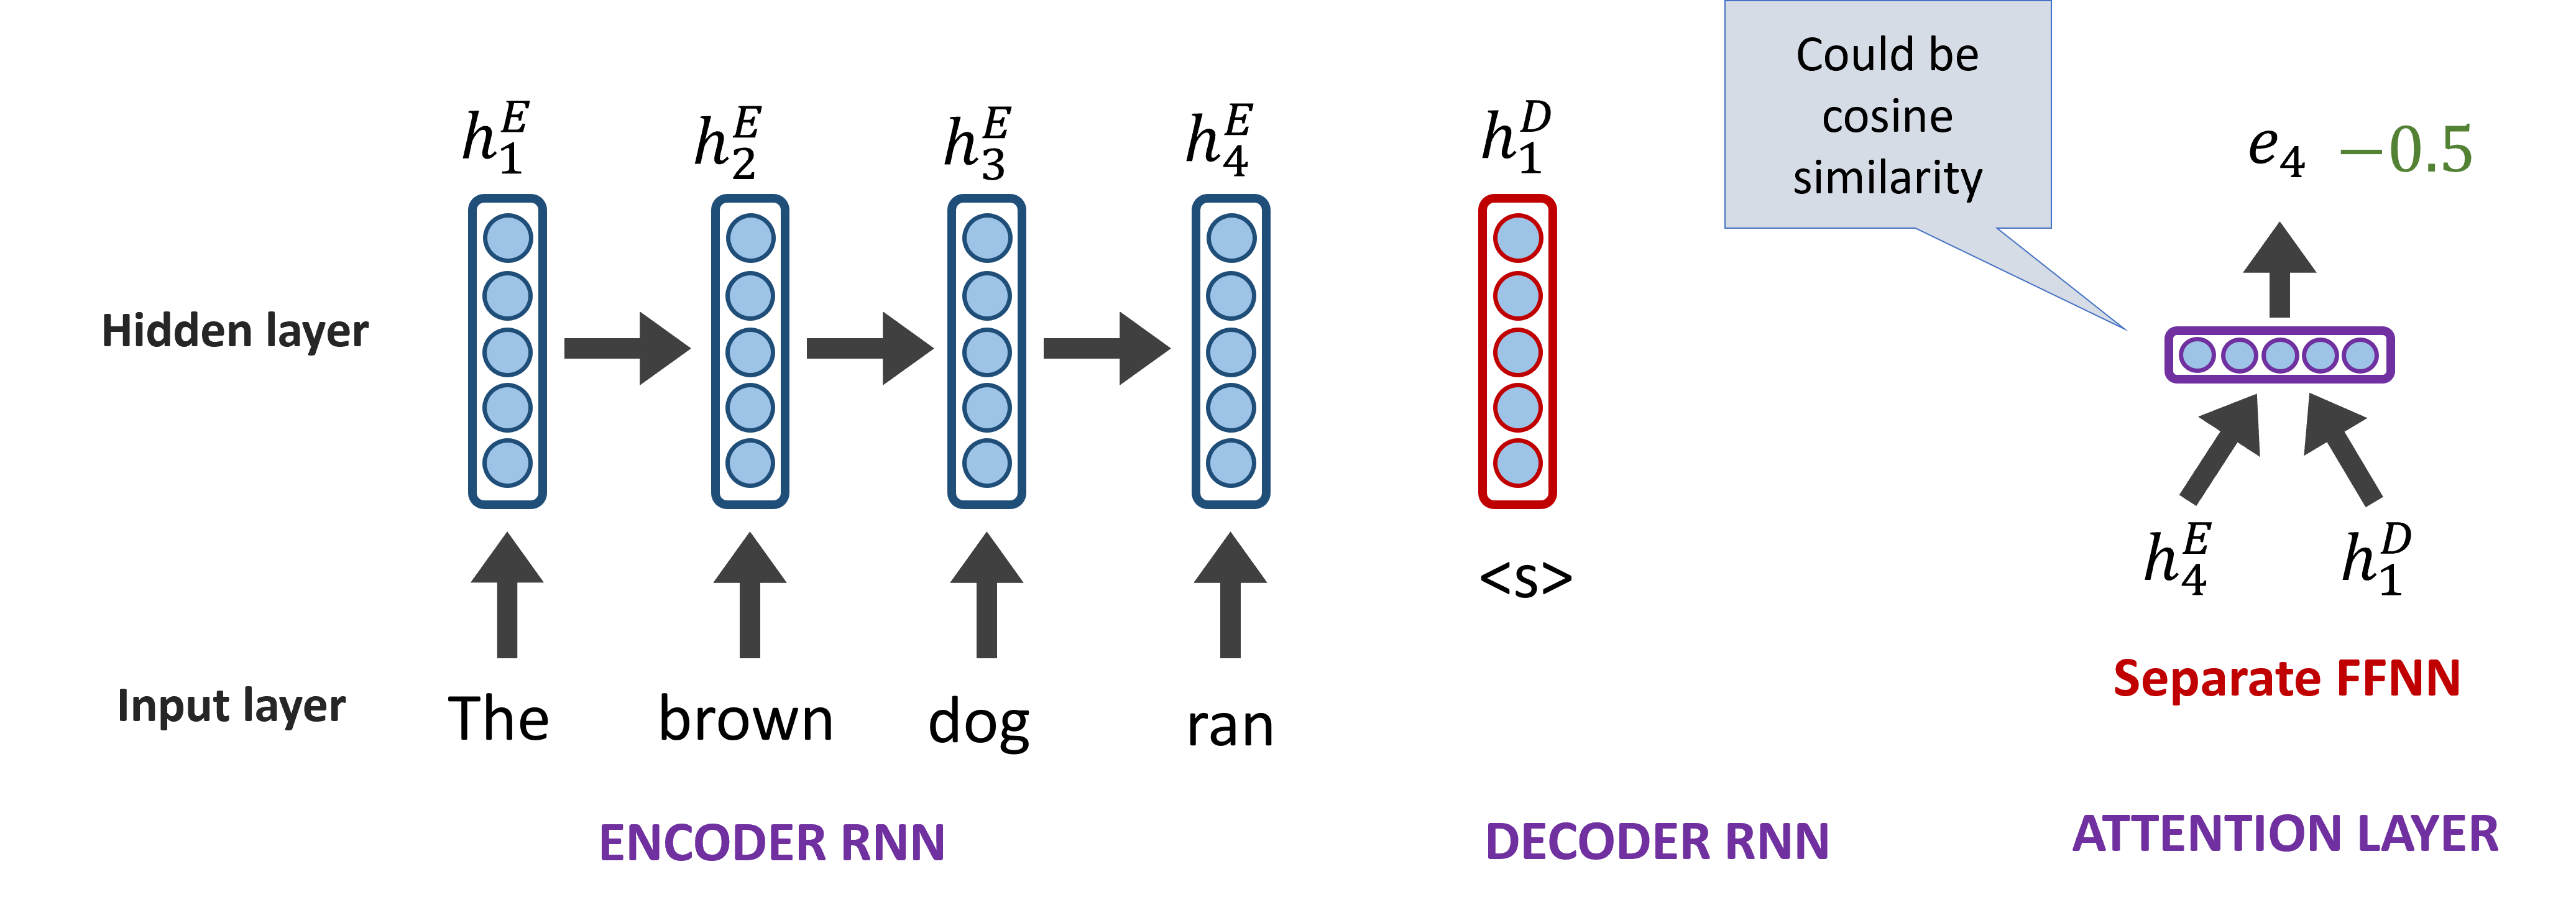
\includegraphics[width=0.8\linewidth,keepaspectratio]{bert21}
\end{center}	

\end{frame}

%%%%%%%%%%%%%%%%%%%%%%%%%%%%%%%%%%%%%%%%%%%%%%%%%%%%%%%%%%%
\begin{frame}[fragile]\frametitle{seq2seq + Attention}

Q: How do we determine how much to pay attention to each of the encoder’s hidden layers? 

A: Let’s base it on our decoder’s previous hidden state (our latest representation of meaning) and all of the encoder’s hidden layers!



\begin{center}
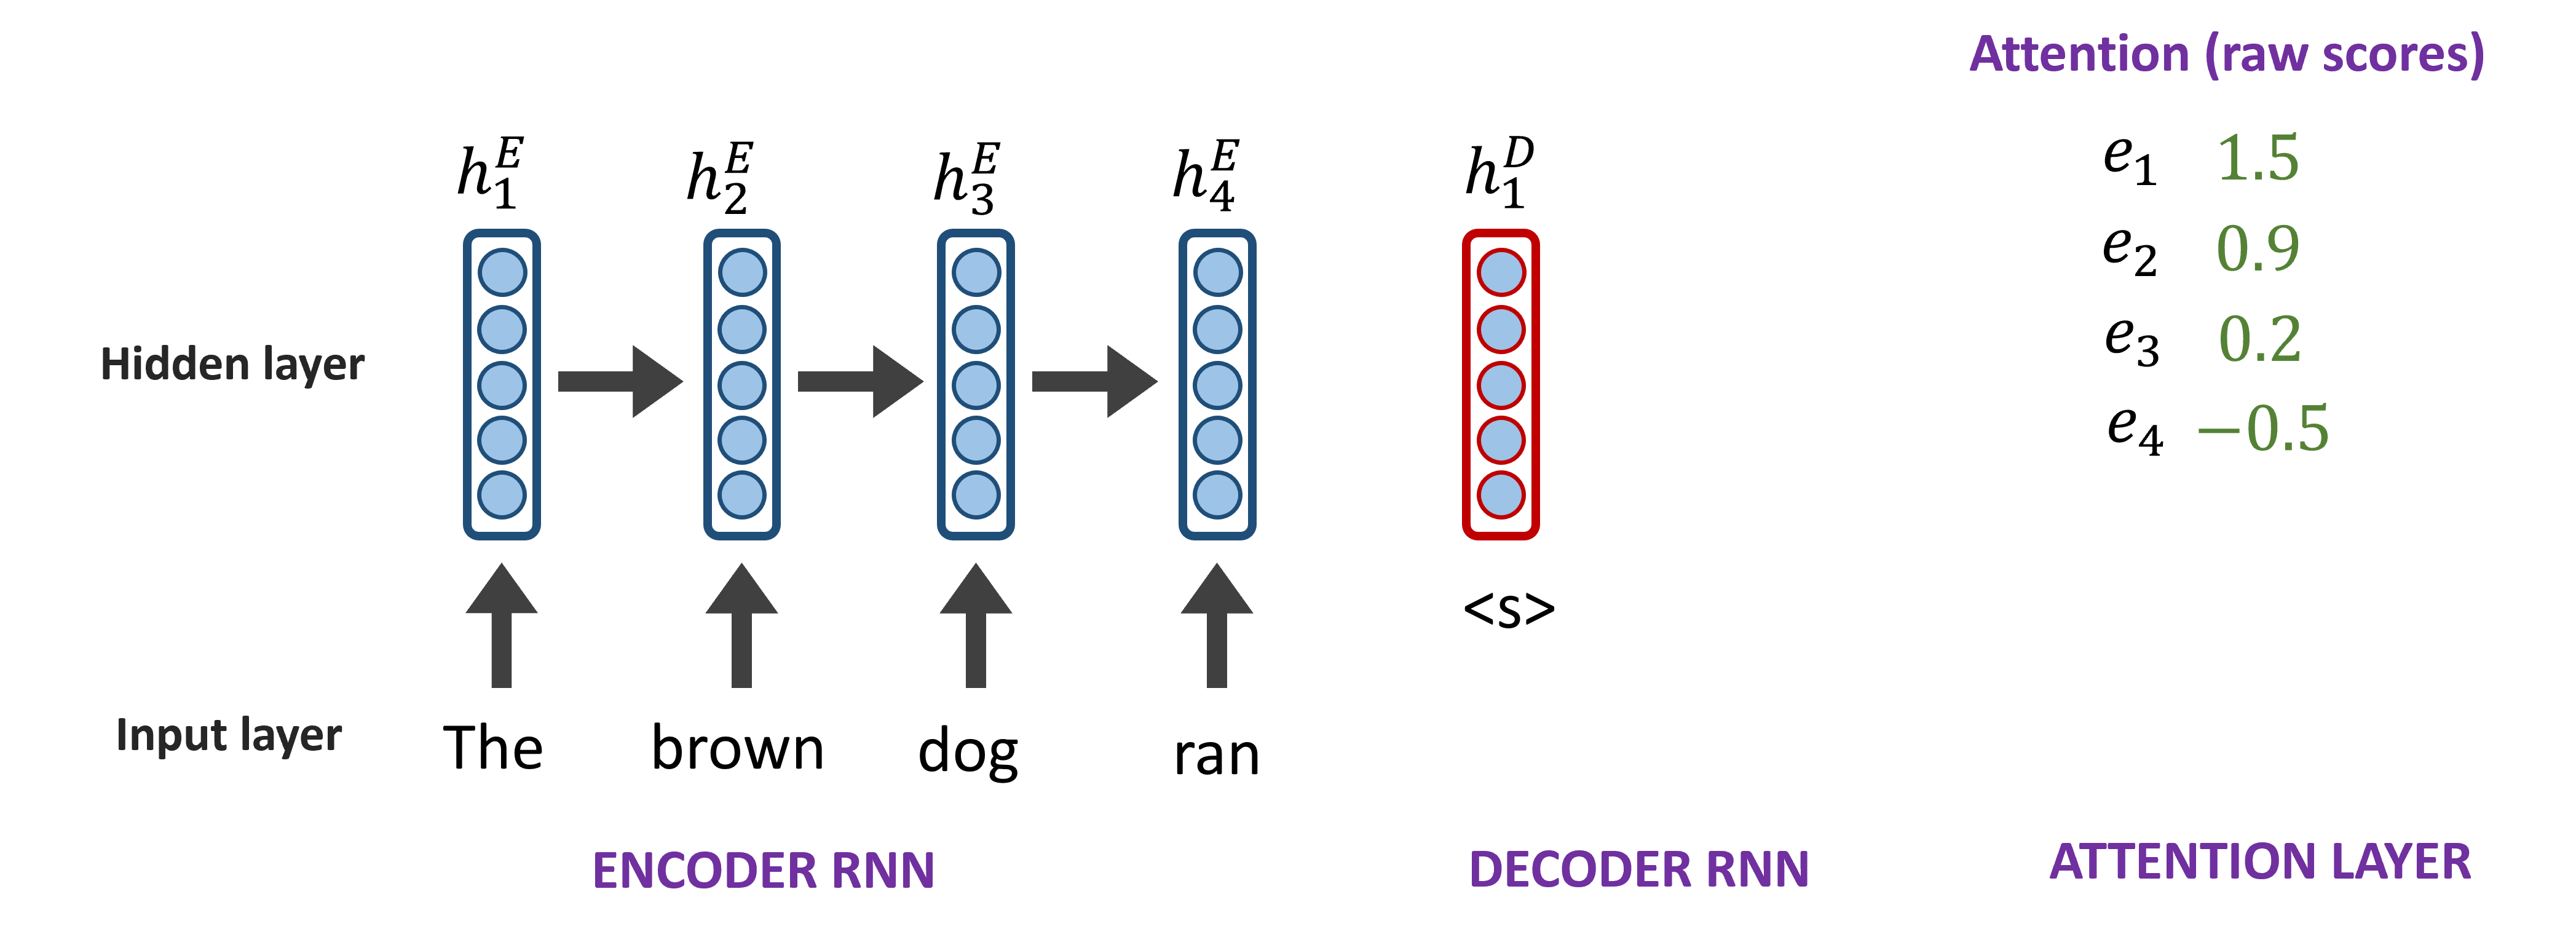
\includegraphics[width=0.8\linewidth,keepaspectratio]{bert22}
\end{center}	

\end{frame}

%%%%%%%%%%%%%%%%%%%%%%%%%%%%%%%%%%%%%%%%%%%%%%%%%%%%%%%%%%%
\begin{frame}[fragile]\frametitle{seq2seq + Attention}

Q: How do we determine how much to pay attention to each of the encoder’s hidden layers? 

A: Let’s base it on our decoder’s previous hidden state (our latest representation of meaning) and all of the encoder’s hidden layers!



\begin{center}
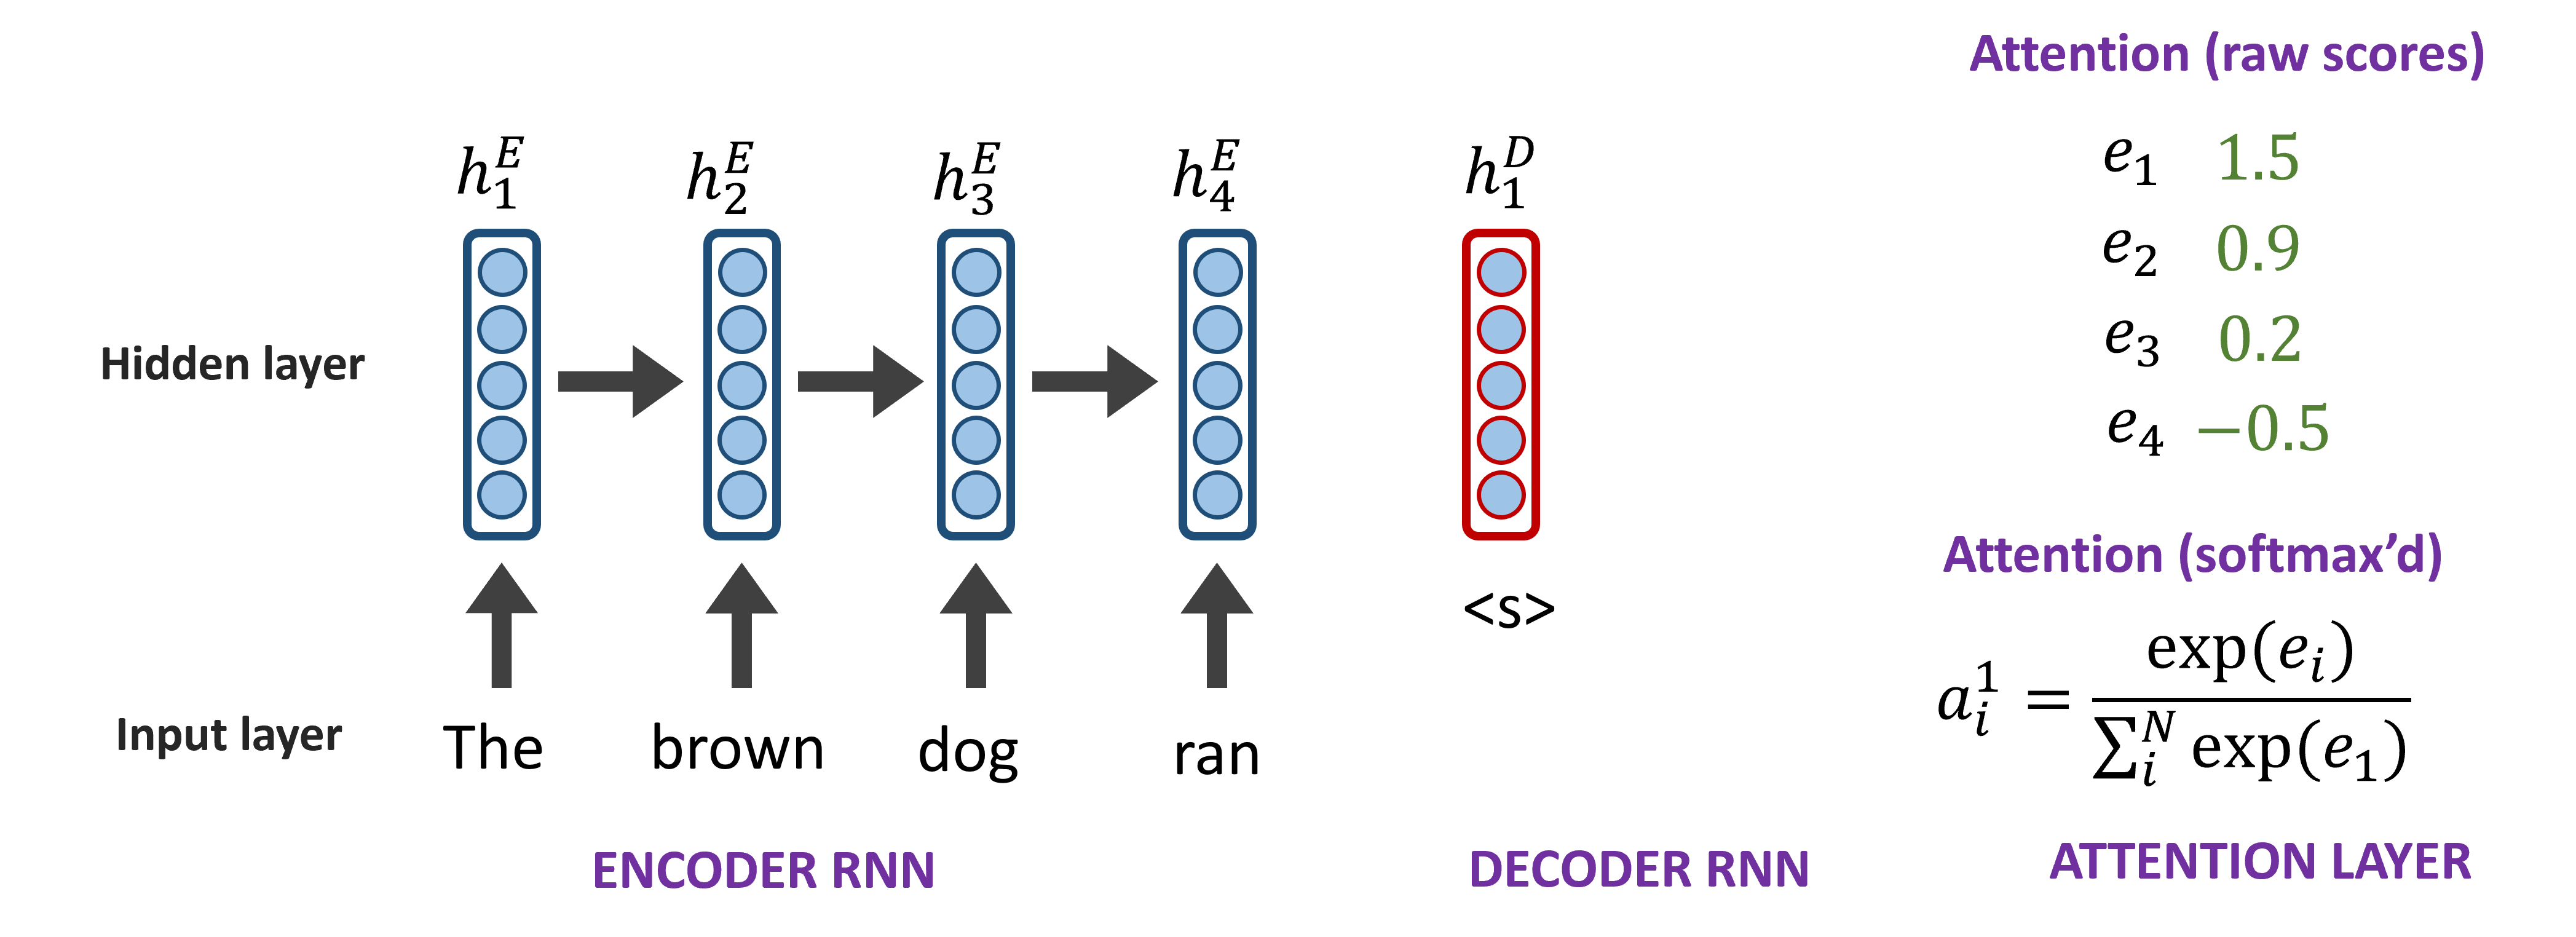
\includegraphics[width=0.8\linewidth,keepaspectratio]{bert23}
\end{center}	

\end{frame}

%%%%%%%%%%%%%%%%%%%%%%%%%%%%%%%%%%%%%%%%%%%%%%%%%%%%%%%%%%%
\begin{frame}[fragile]\frametitle{seq2seq + Attention}

Q: How do we determine how much to pay attention to each of the encoder’s hidden layers? 

A: Let’s base it on our decoder’s previous hidden state (our latest representation of meaning) and all of the encoder’s hidden layers!



\begin{center}
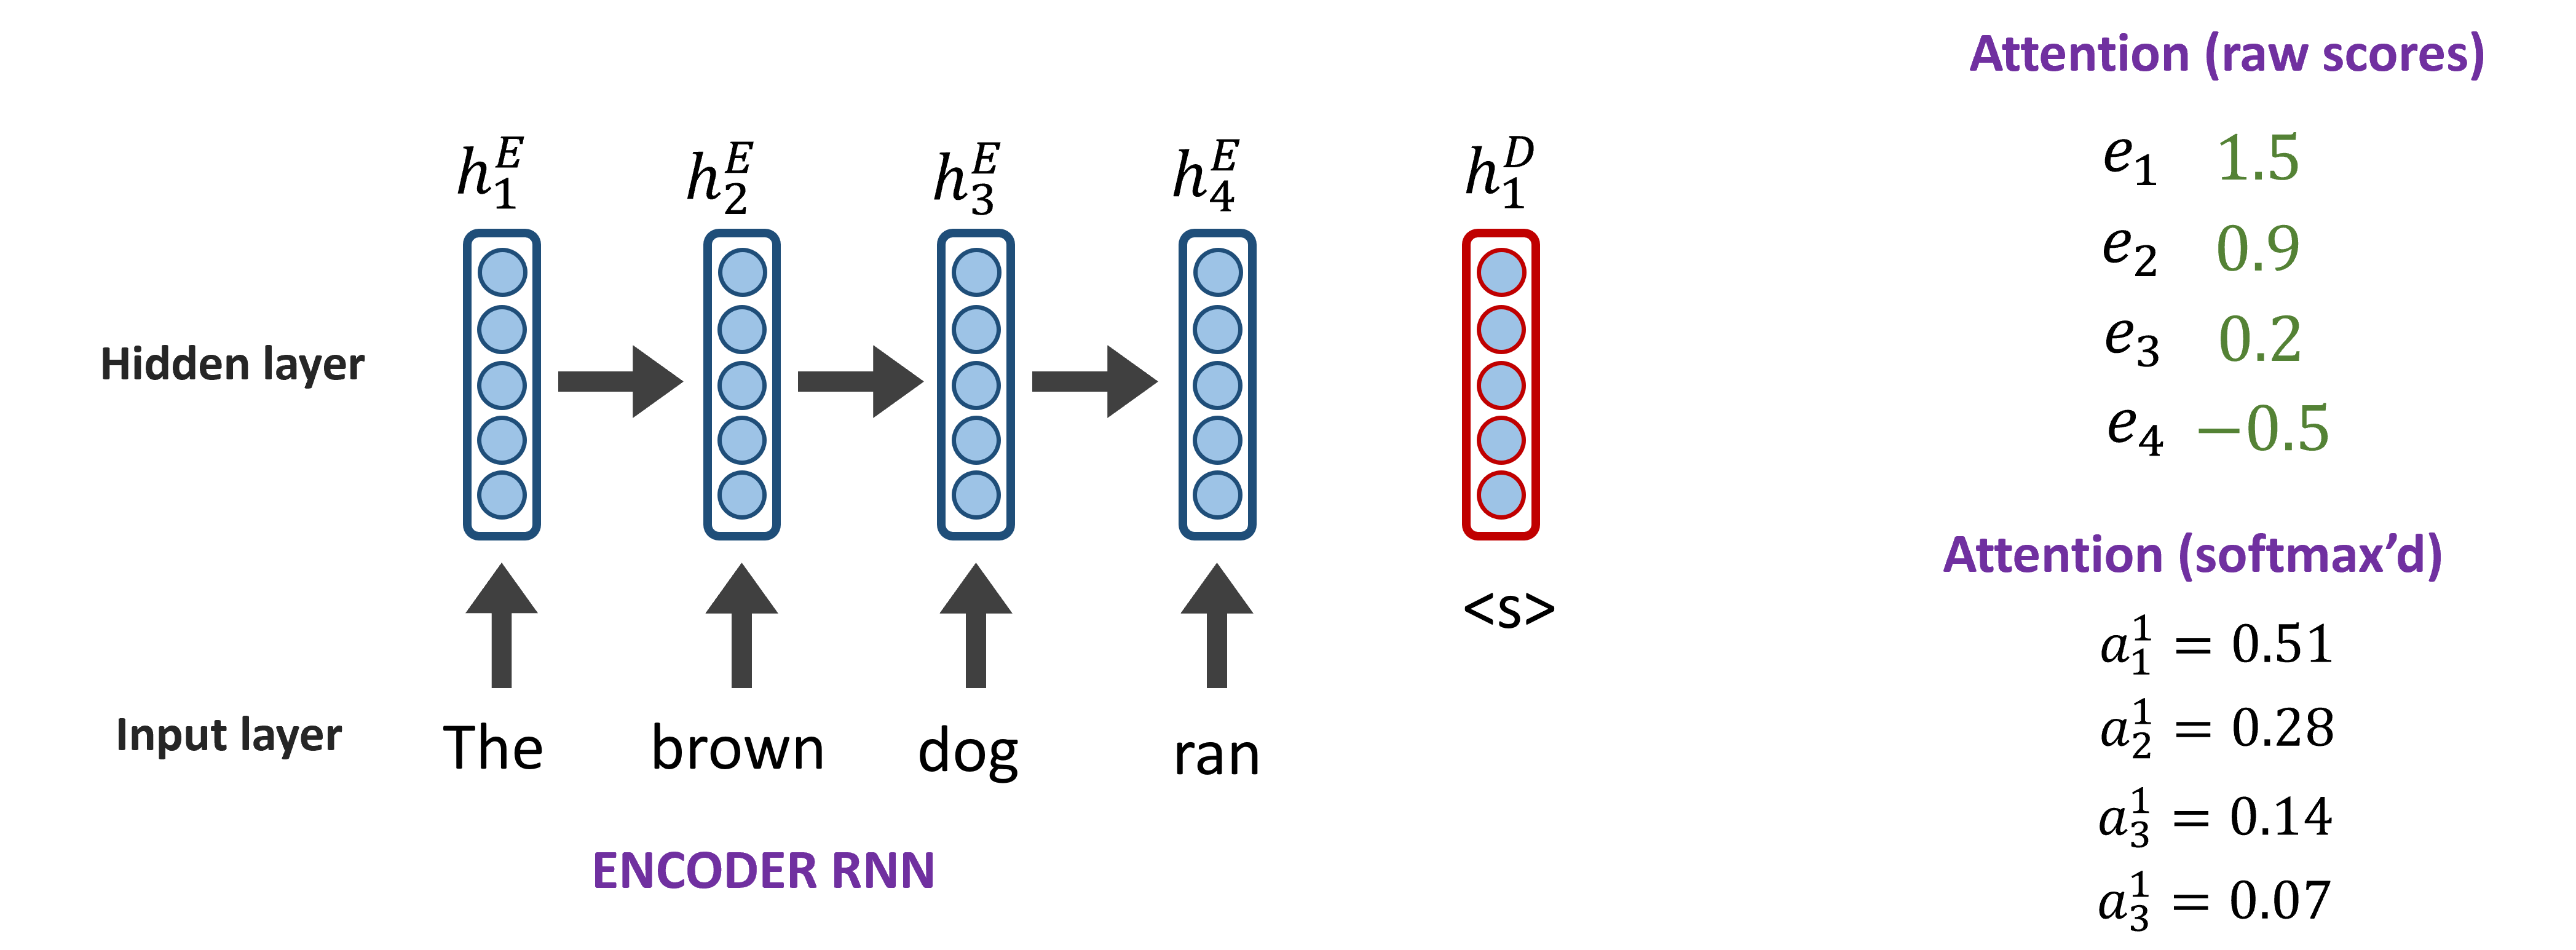
\includegraphics[width=0.8\linewidth,keepaspectratio]{bert24}
\end{center}	

\end{frame}

%%%%%%%%%%%%%%%%%%%%%%%%%%%%%%%%%%%%%%%%%%%%%%%%%%%%%%%%%%%
\begin{frame}[fragile]\frametitle{seq2seq + Attention}

\begin{center}
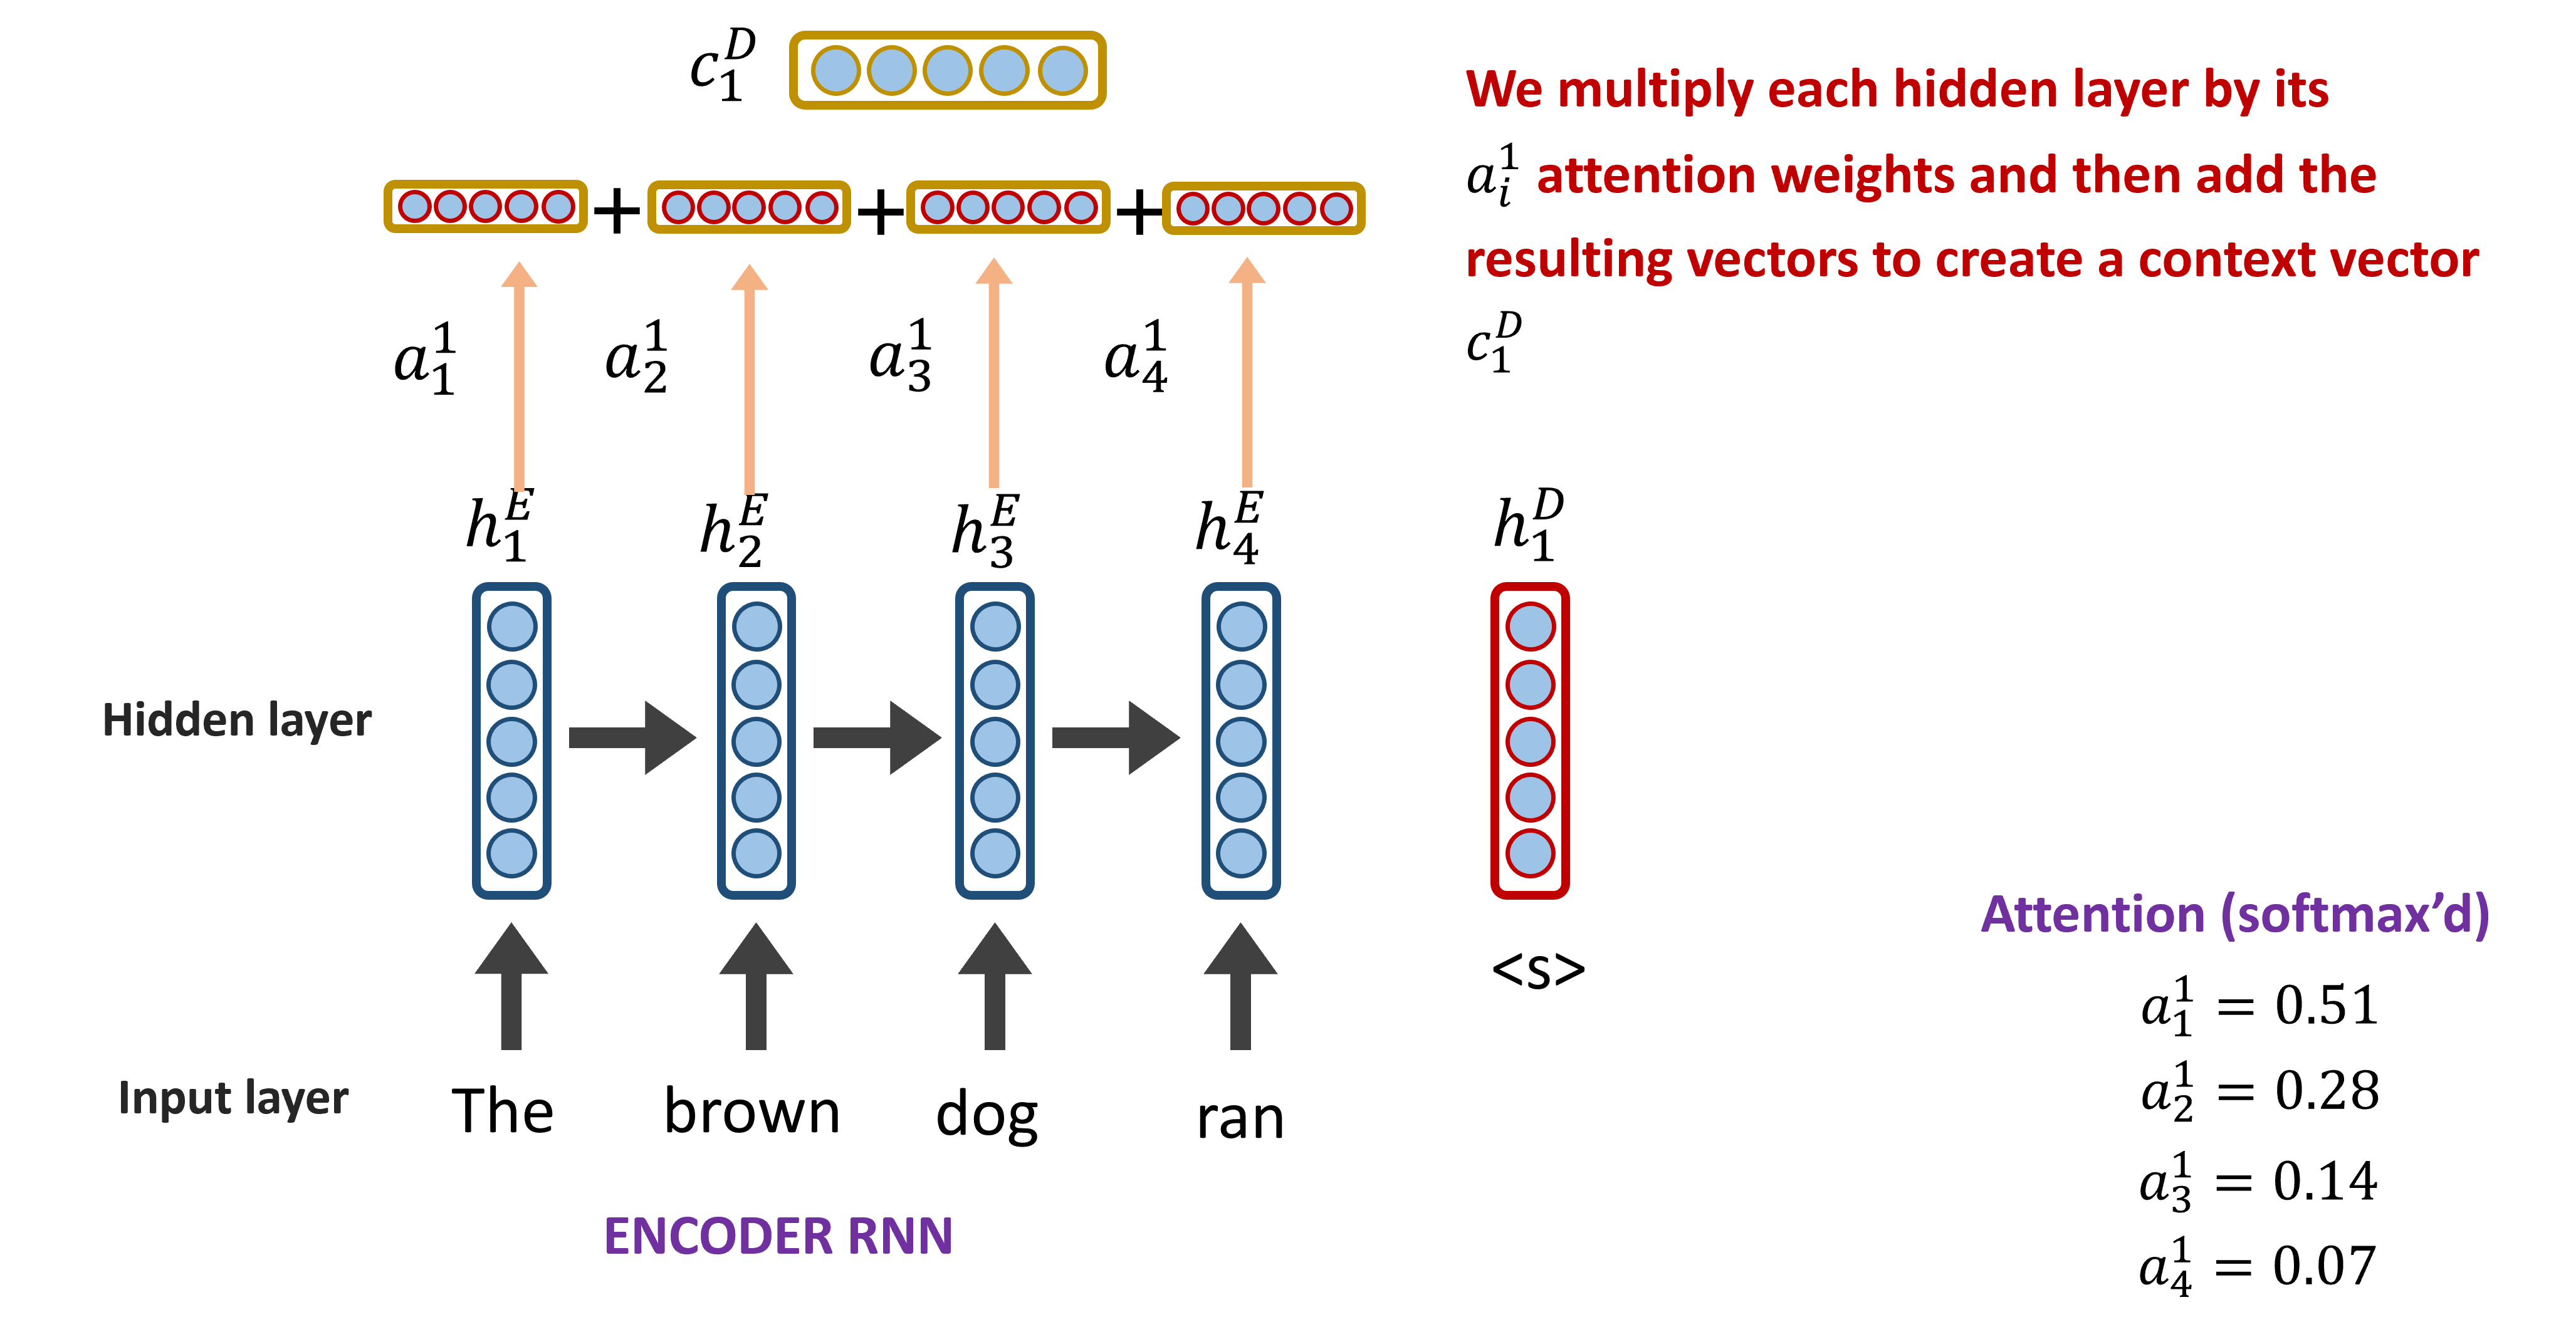
\includegraphics[width=0.8\linewidth,keepaspectratio]{bert25}
\end{center}	

\end{frame}

%%%%%%%%%%%%%%%%%%%%%%%%%%%%%%%%%%%%%%%%%%%%%%%%%%%%%%%%%%%
\begin{frame}[fragile]\frametitle{seq2seq + Attention}

\begin{center}
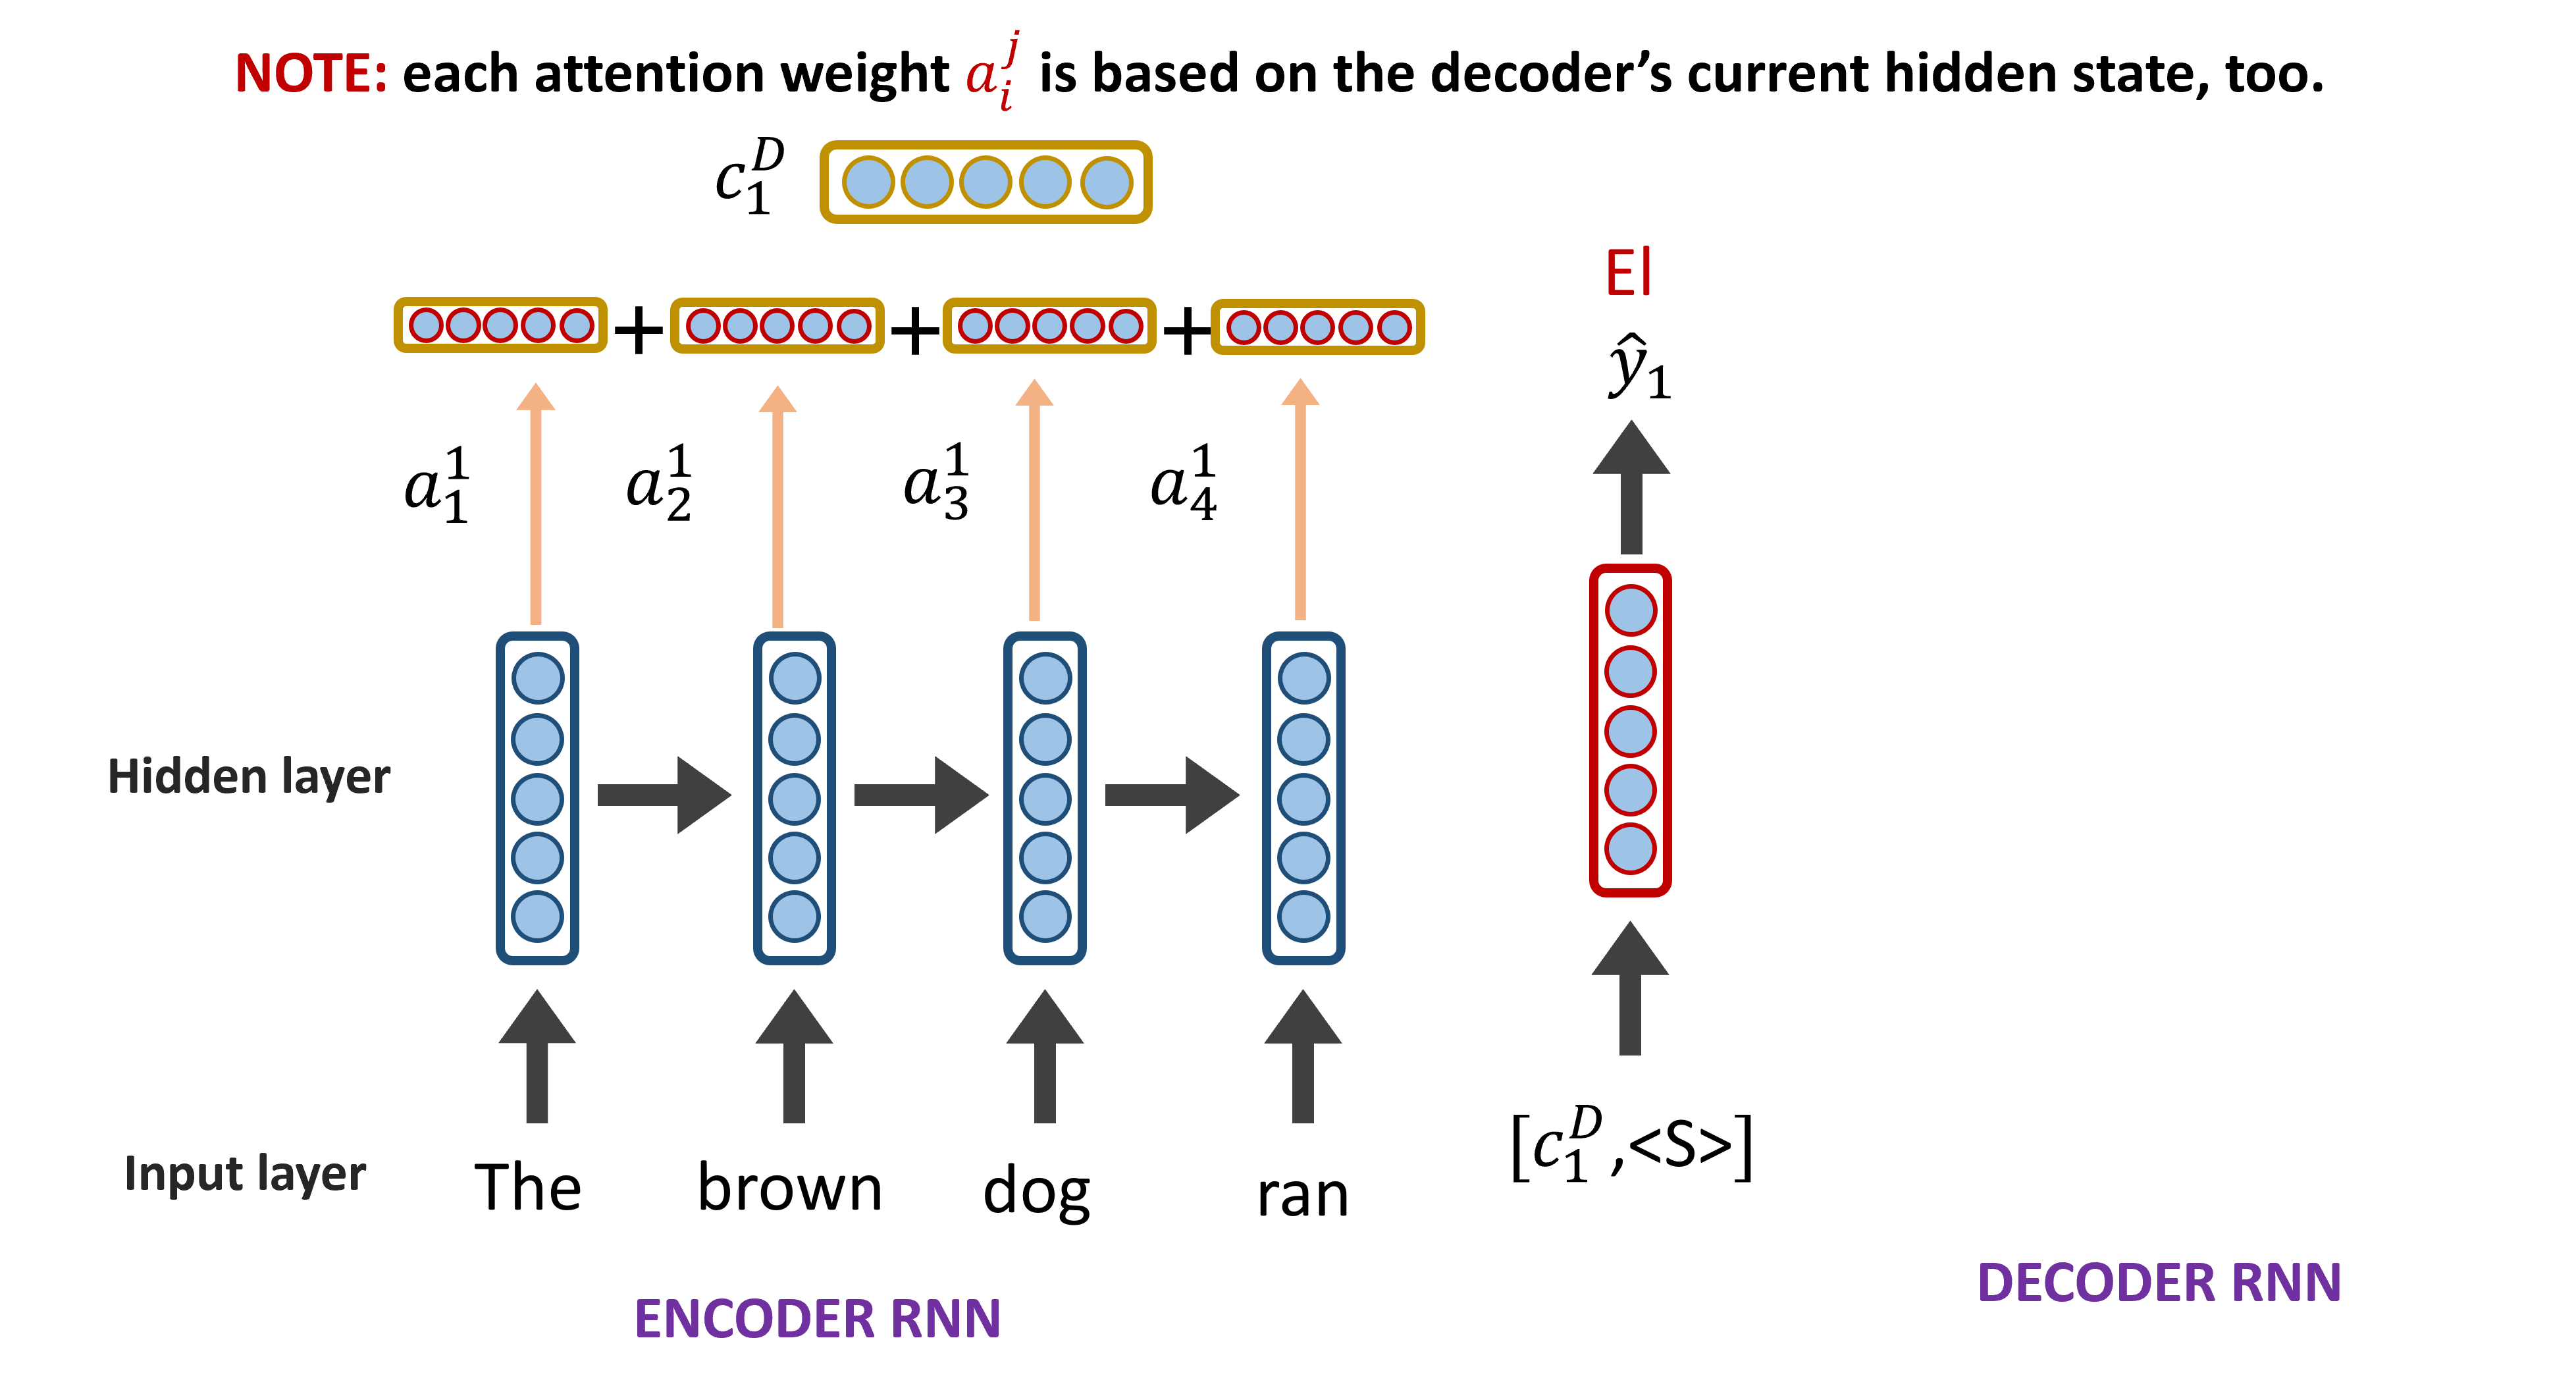
\includegraphics[width=0.8\linewidth,keepaspectratio]{bert26}
\end{center}	

\end{frame}

%%%%%%%%%%%%%%%%%%%%%%%%%%%%%%%%%%%%%%%%%%%%%%%%%%%%%%%%%%%
\begin{frame}[fragile]\frametitle{seq2seq + Attention}

\begin{center}
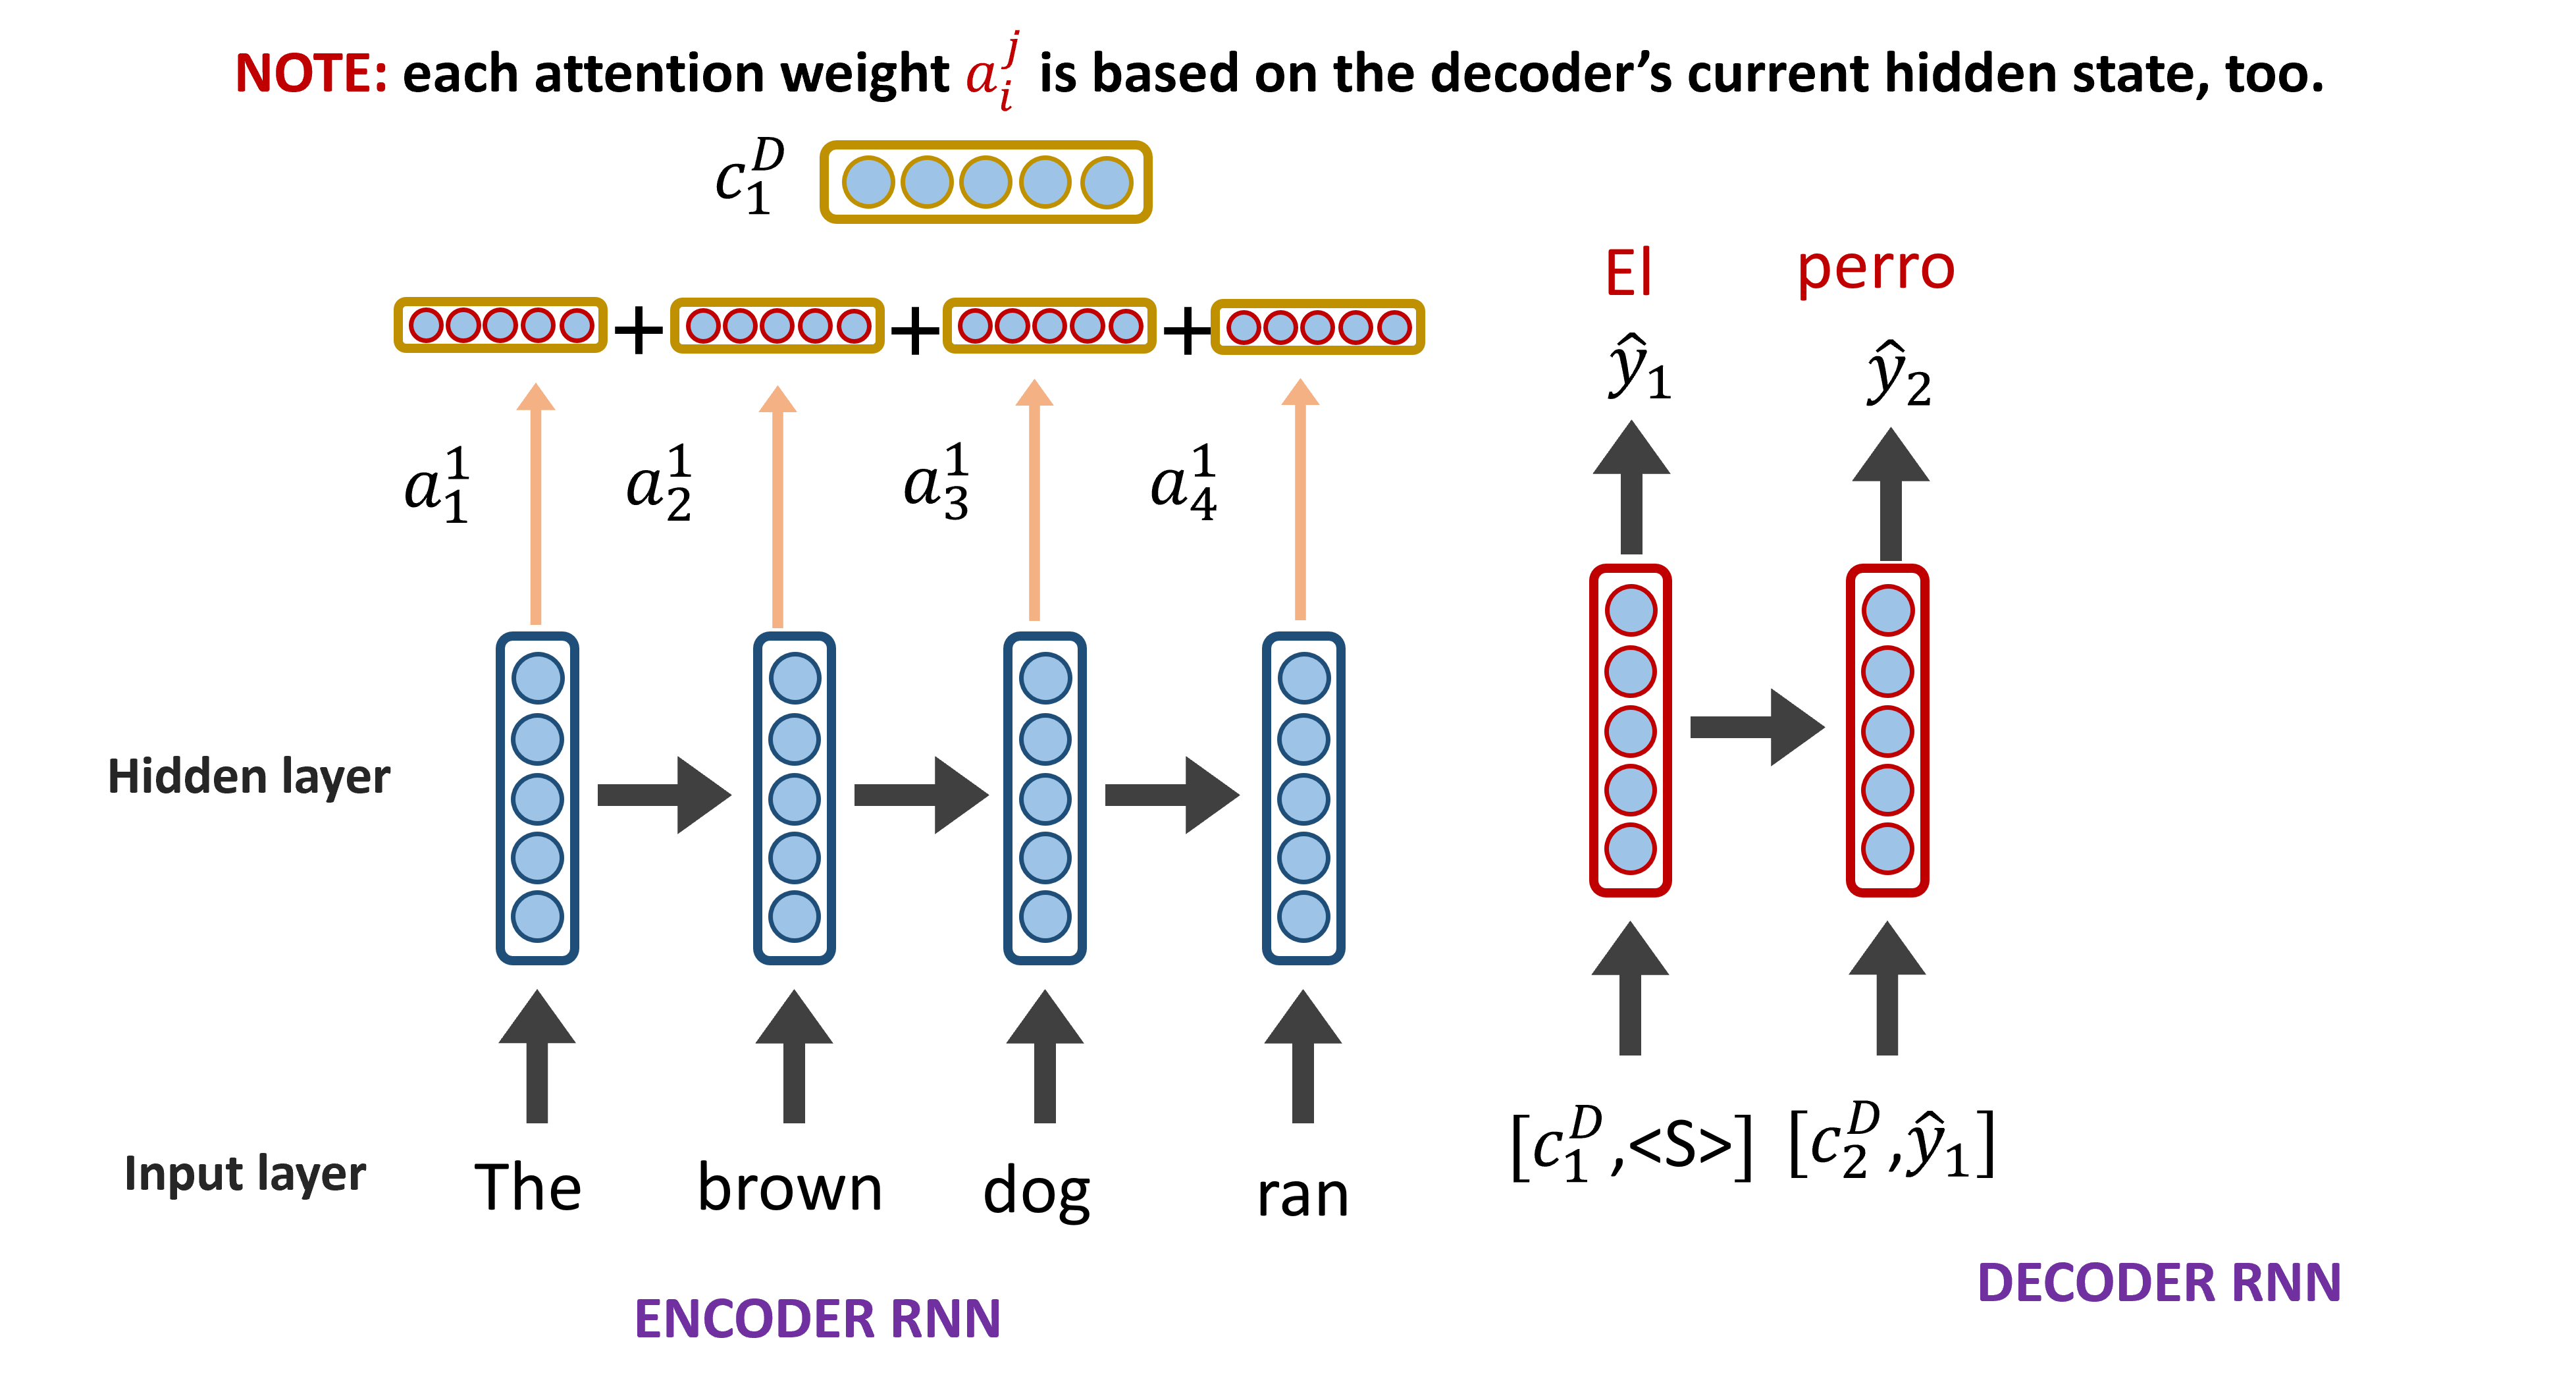
\includegraphics[width=0.8\linewidth,keepaspectratio]{bert27}
\end{center}	

\end{frame}


%%%%%%%%%%%%%%%%%%%%%%%%%%%%%%%%%%%%%%%%%%%%%%%%%%%%%%%%%%%
\begin{frame}[fragile]\frametitle{seq2seq + Attention}

\begin{center}
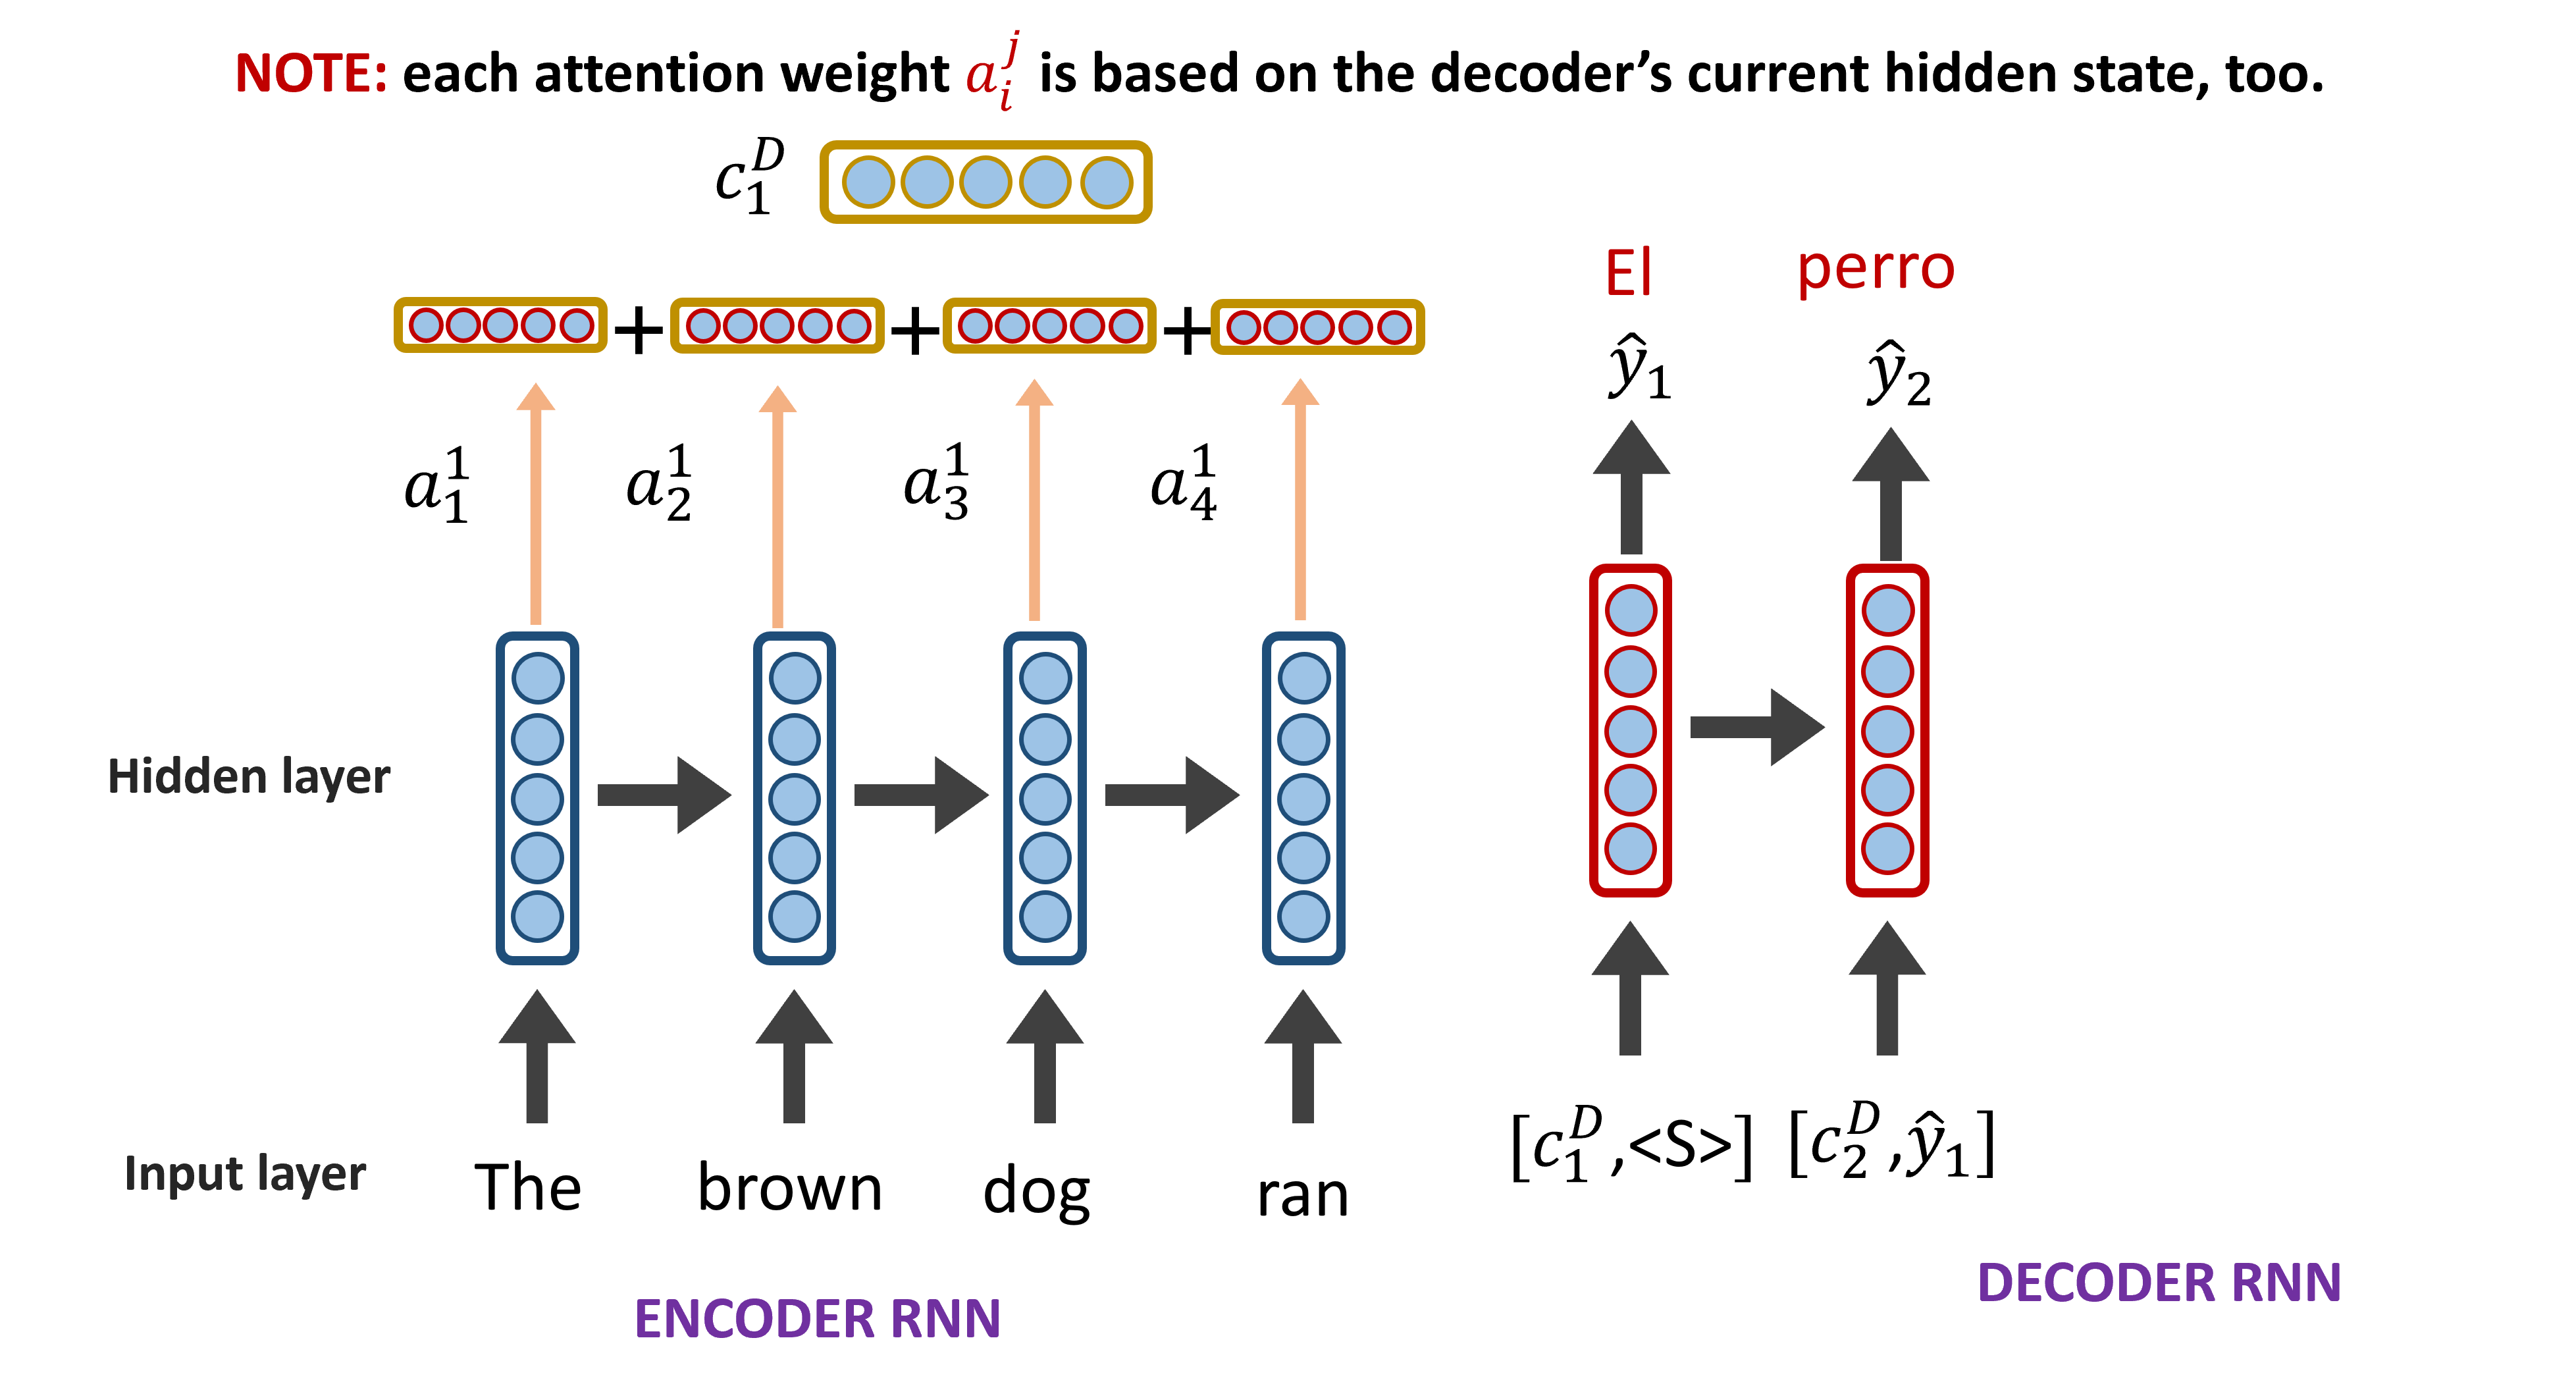
\includegraphics[width=0.8\linewidth,keepaspectratio]{bert28}
\end{center}	

\end{frame}

%%%%%%%%%%%%%%%%%%%%%%%%%%%%%%%%%%%%%%%%%%%%%%%%%%%%%%%%%%%
\begin{frame}[fragile]\frametitle{seq2seq + Attention}

\begin{center}
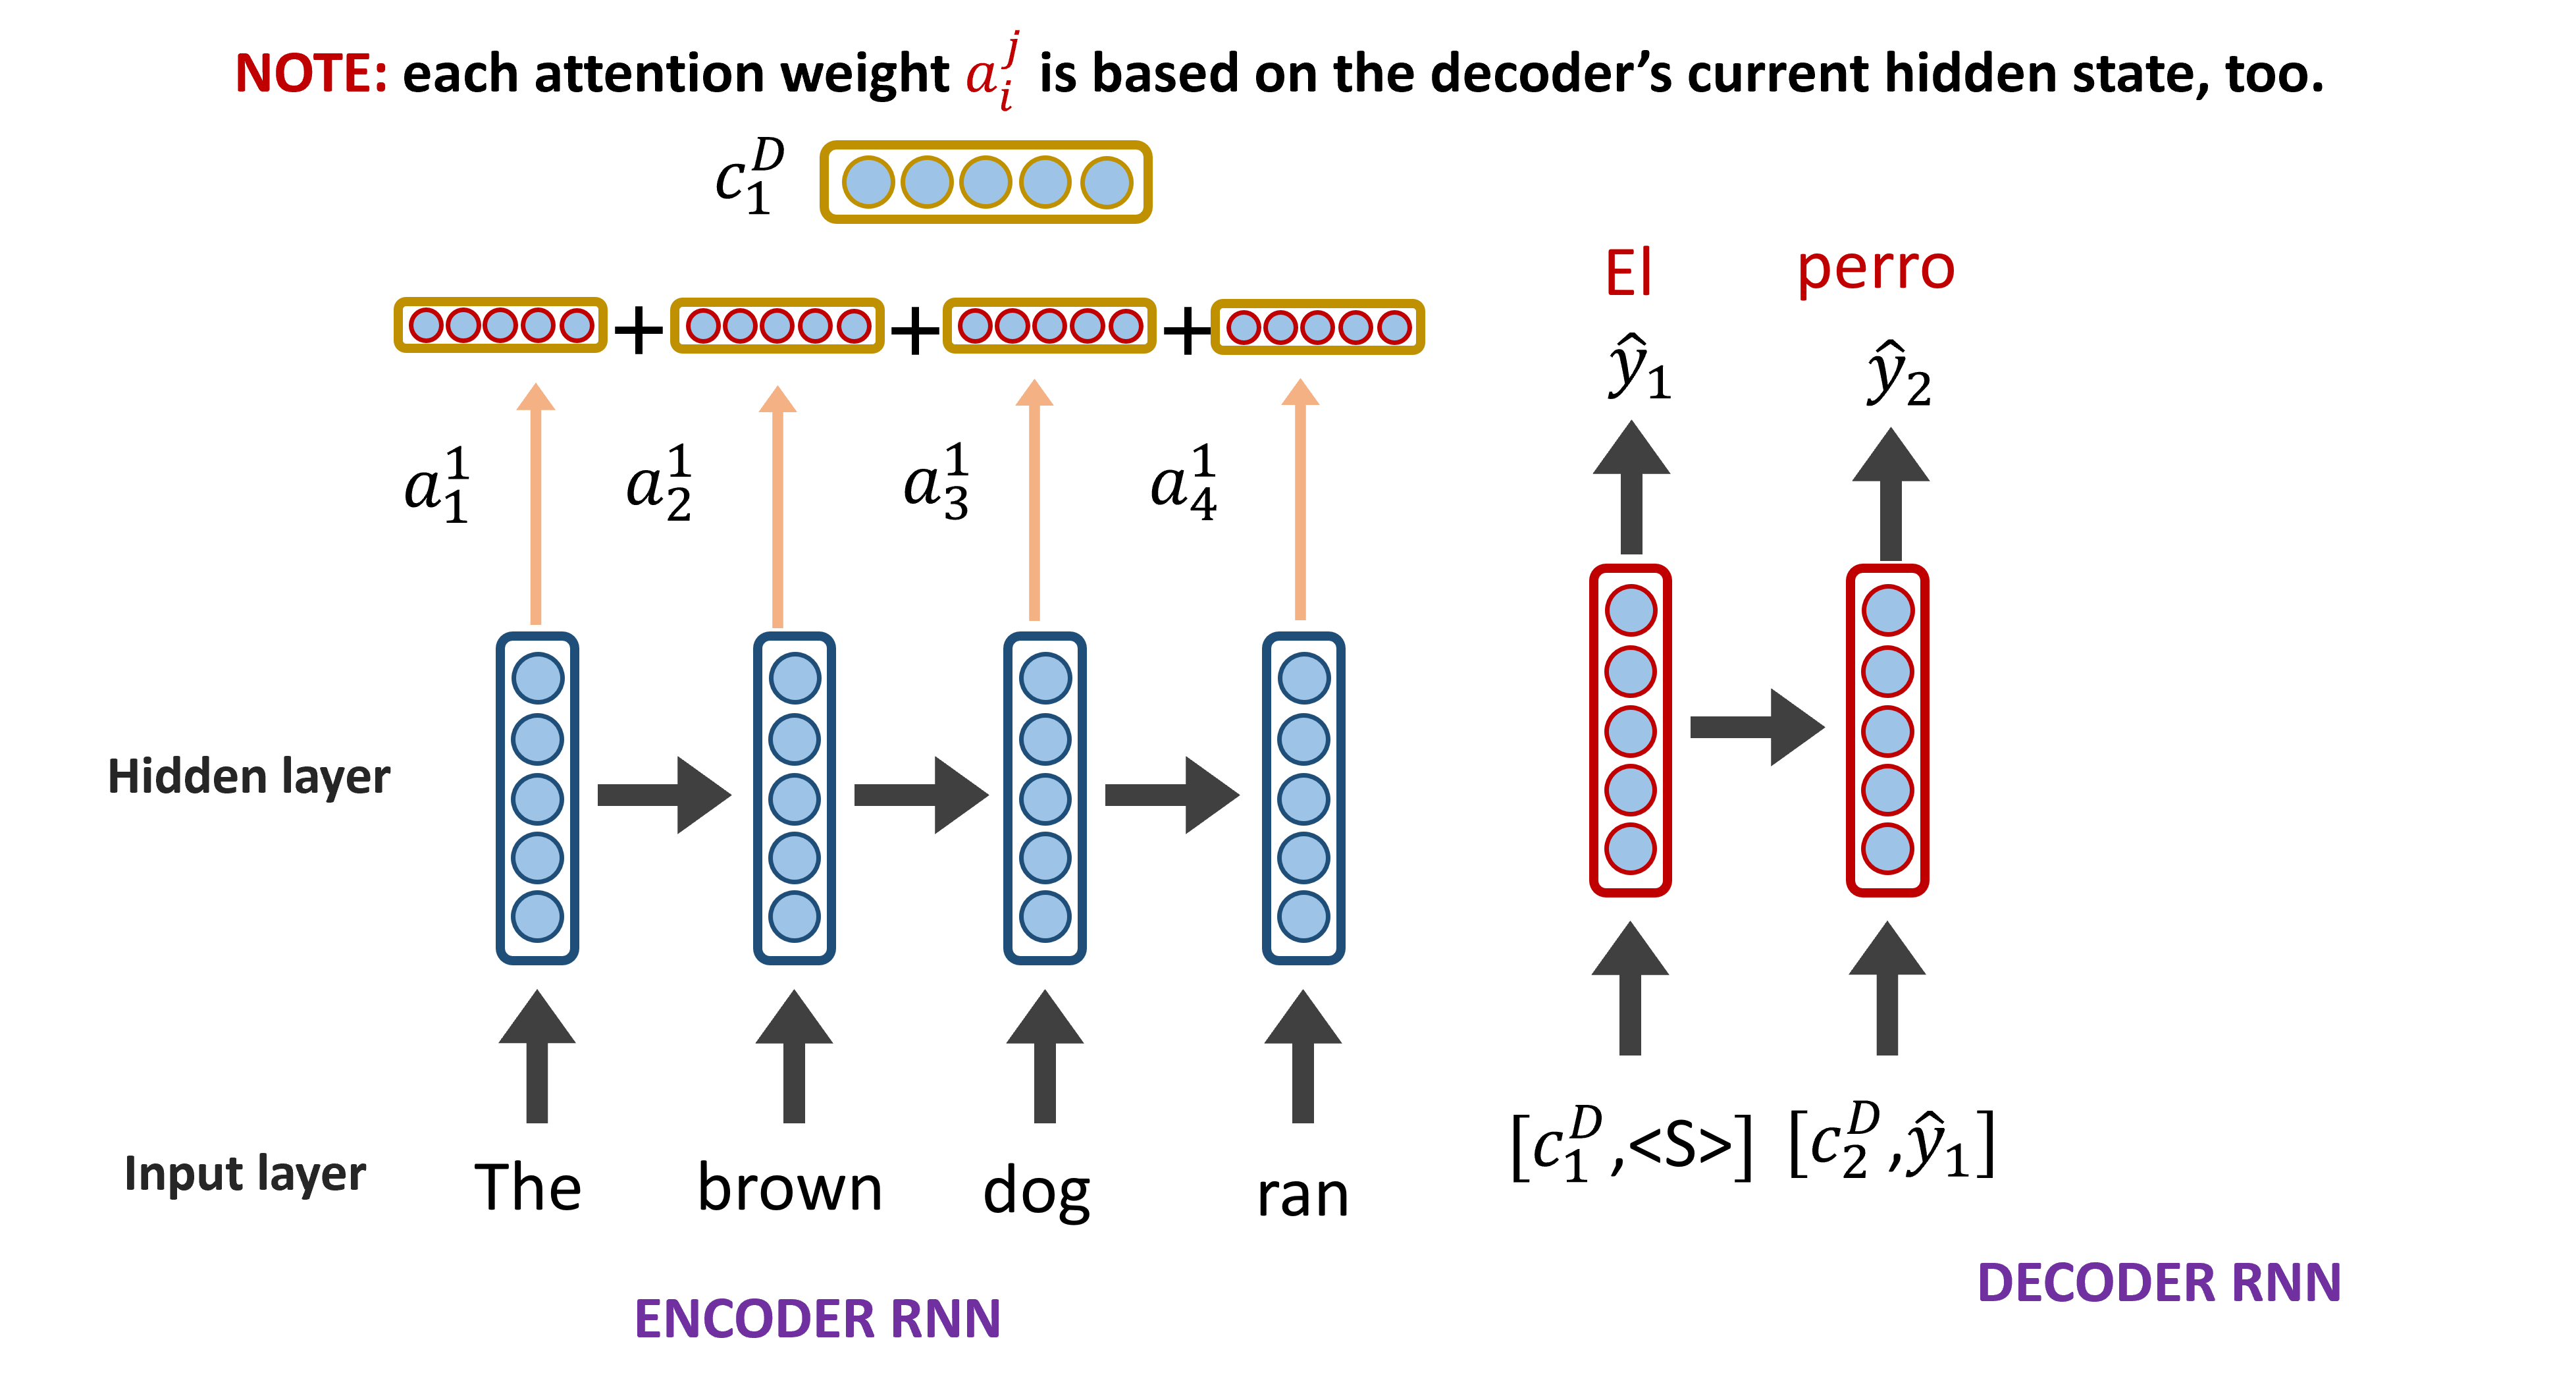
\includegraphics[width=0.8\linewidth,keepaspectratio]{bert29}
\end{center}	

\end{frame}

%%%%%%%%%%%%%%%%%%%%%%%%%%%%%%%%%%%%%%%%%%%%%%%%%%%%%%%%%%%
\begin{frame}[fragile]\frametitle{seq2seq + Attention}

\begin{center}
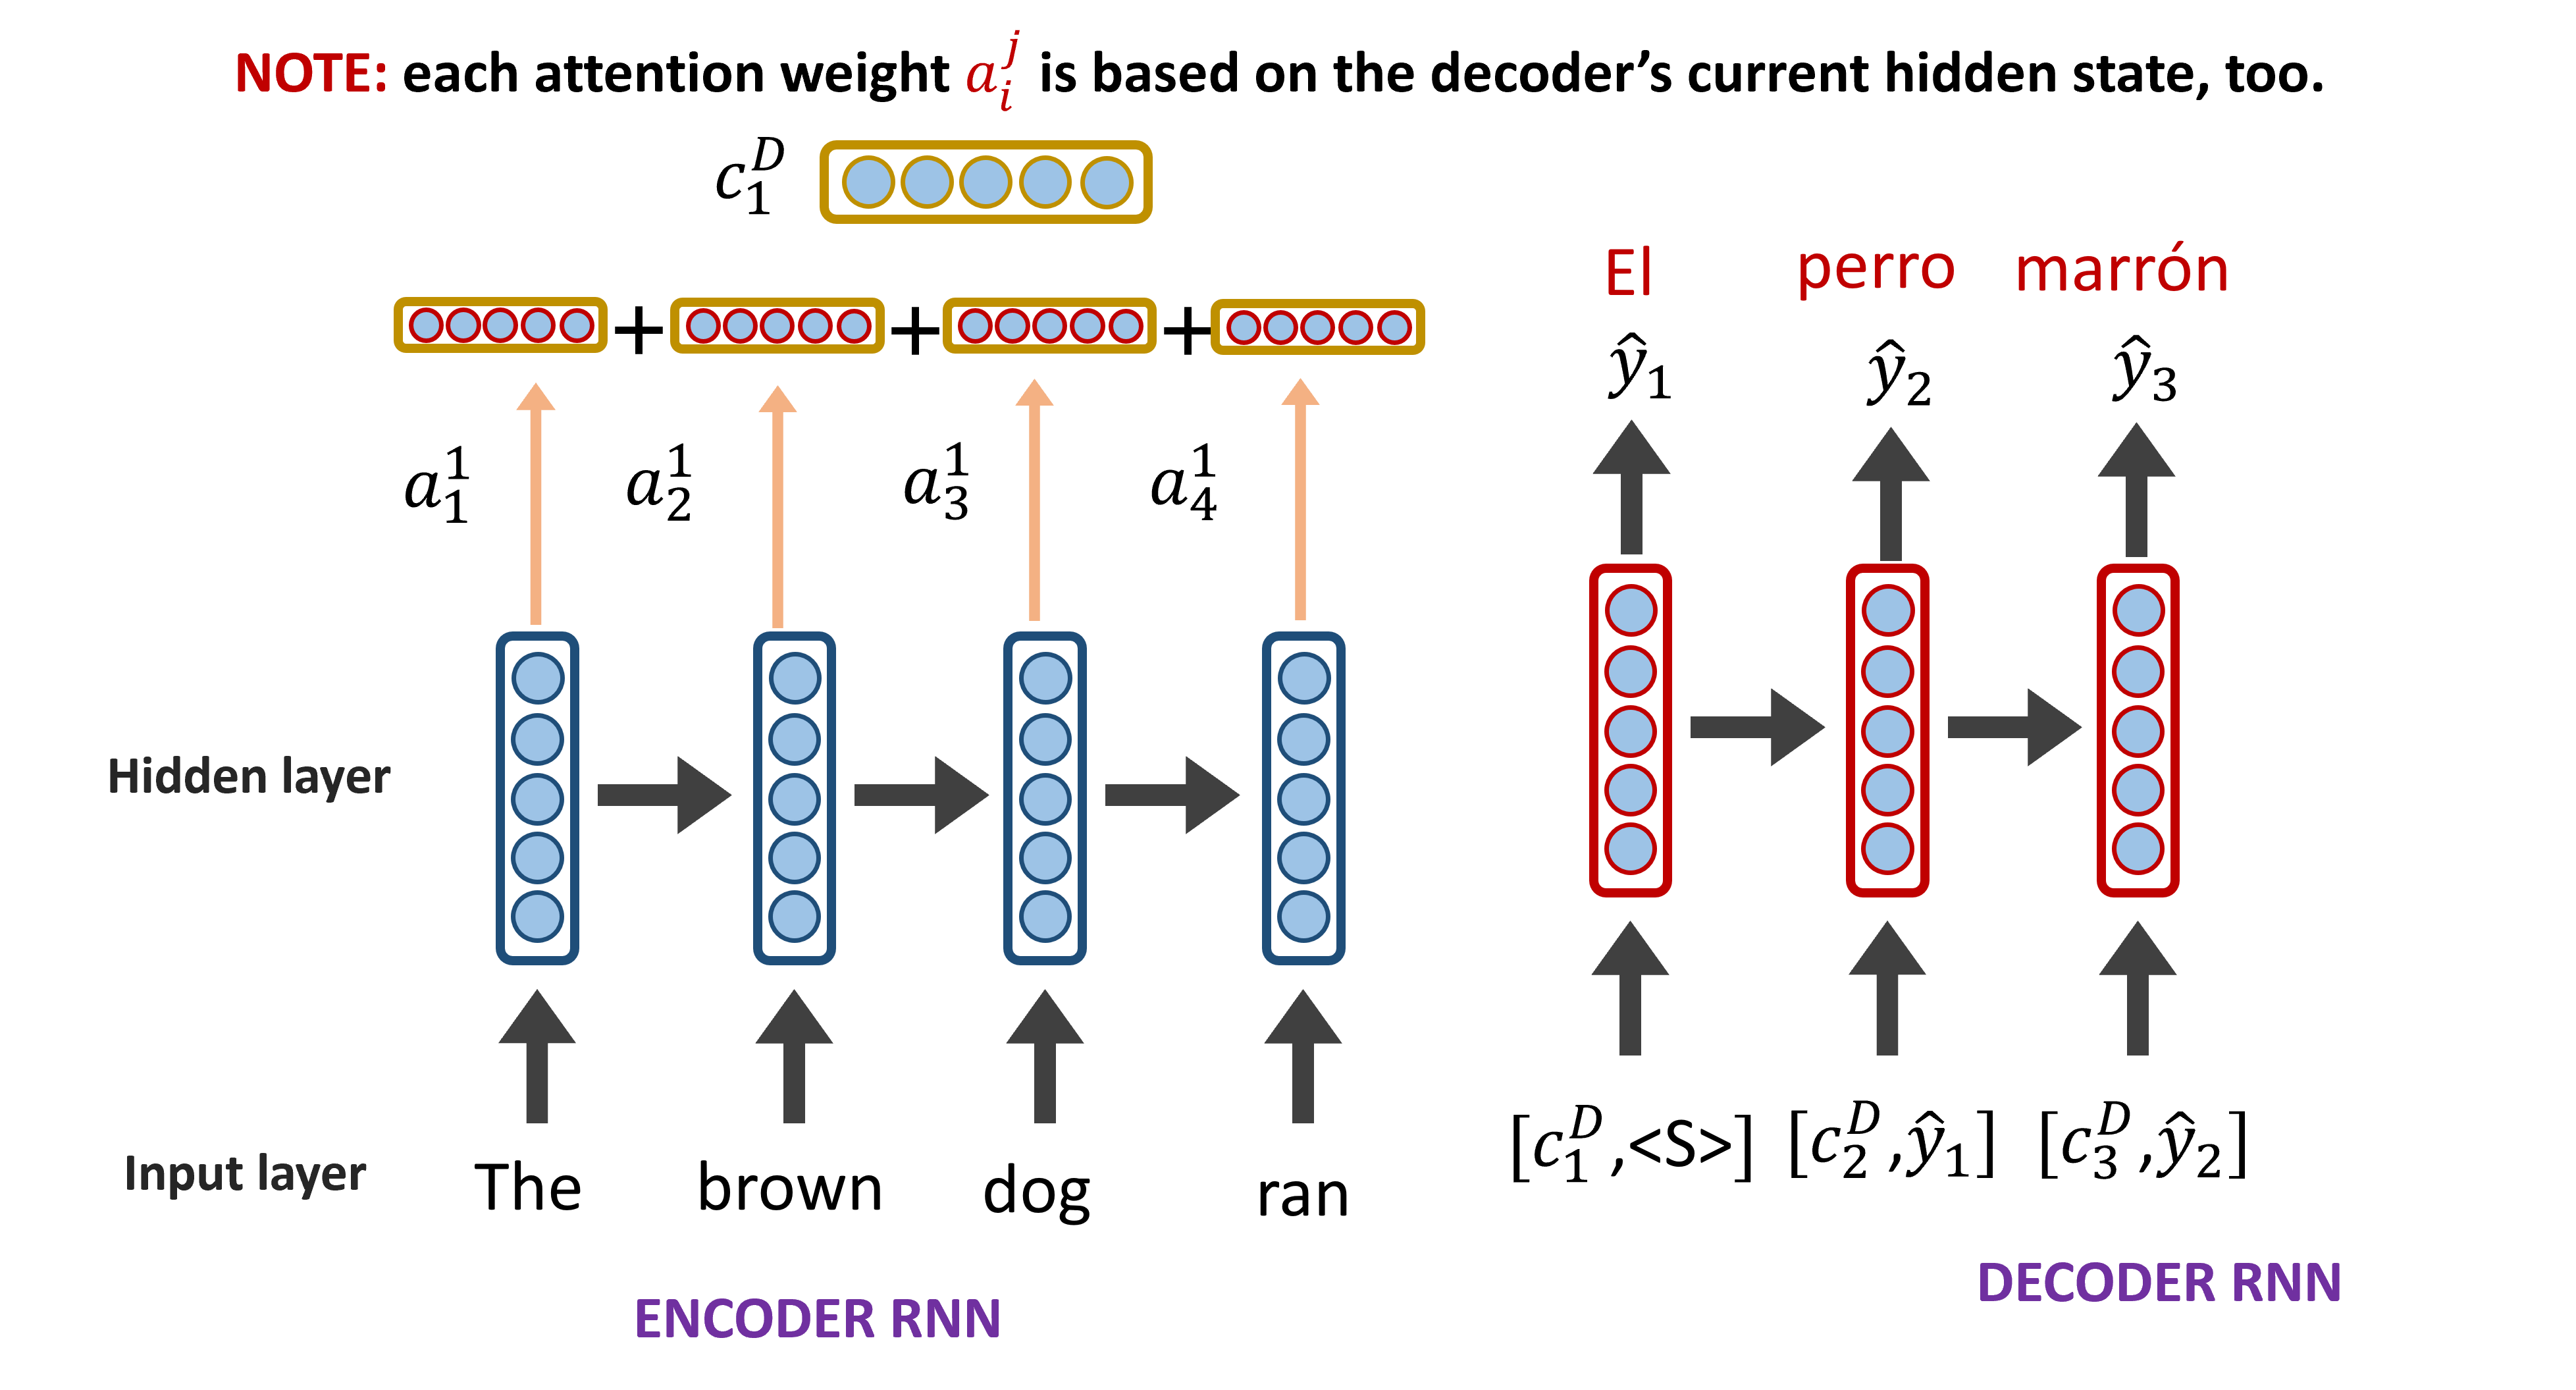
\includegraphics[width=0.8\linewidth,keepaspectratio]{bert30}
\end{center}	

\end{frame}

%%%%%%%%%%%%%%%%%%%%%%%%%%%%%%%%%%%%%%%%%%%%%%%%%%%%%%%%%%%
\begin{frame}[fragile]\frametitle{seq2seq + Attention}

\begin{center}
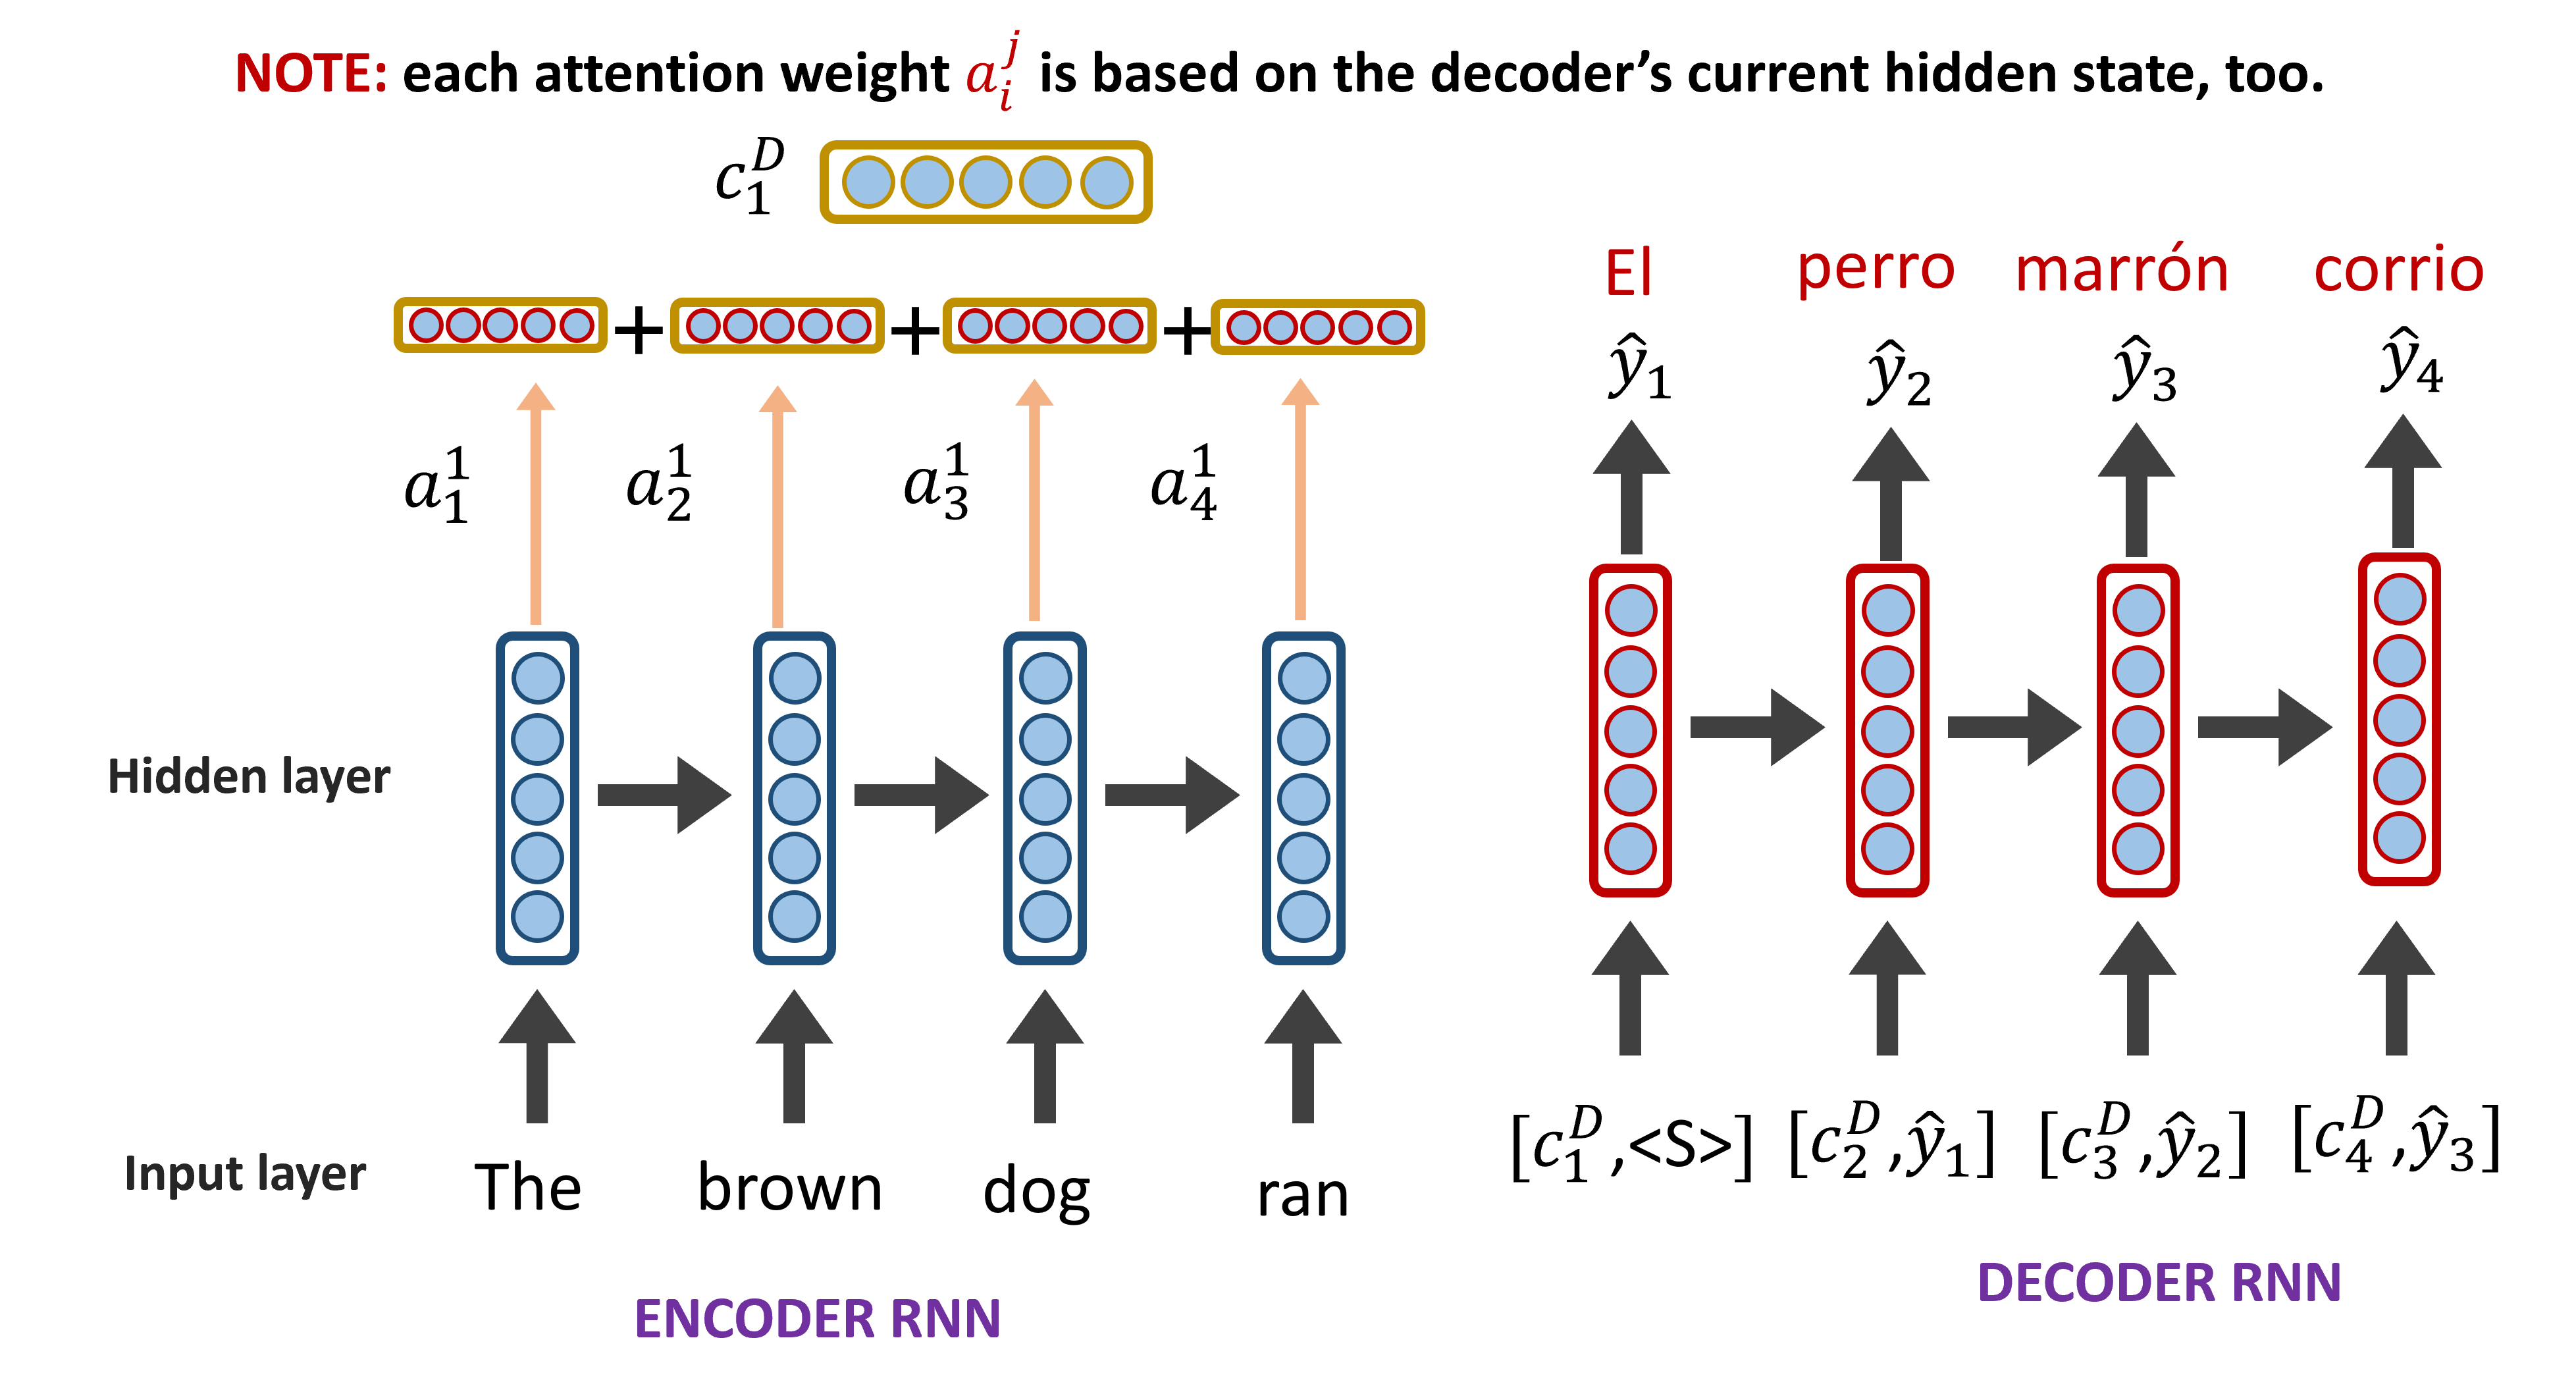
\includegraphics[width=0.8\linewidth,keepaspectratio]{bert31}
\end{center}	

\end{frame}

%%%%%%%%%%%%%%%%%%%%%%%%%%%%%%%%%%%%%%%%%%%%%%%%%%%%%%%%%%%
\begin{frame}[fragile]\frametitle{seq2seq + Attention}

\begin{center}
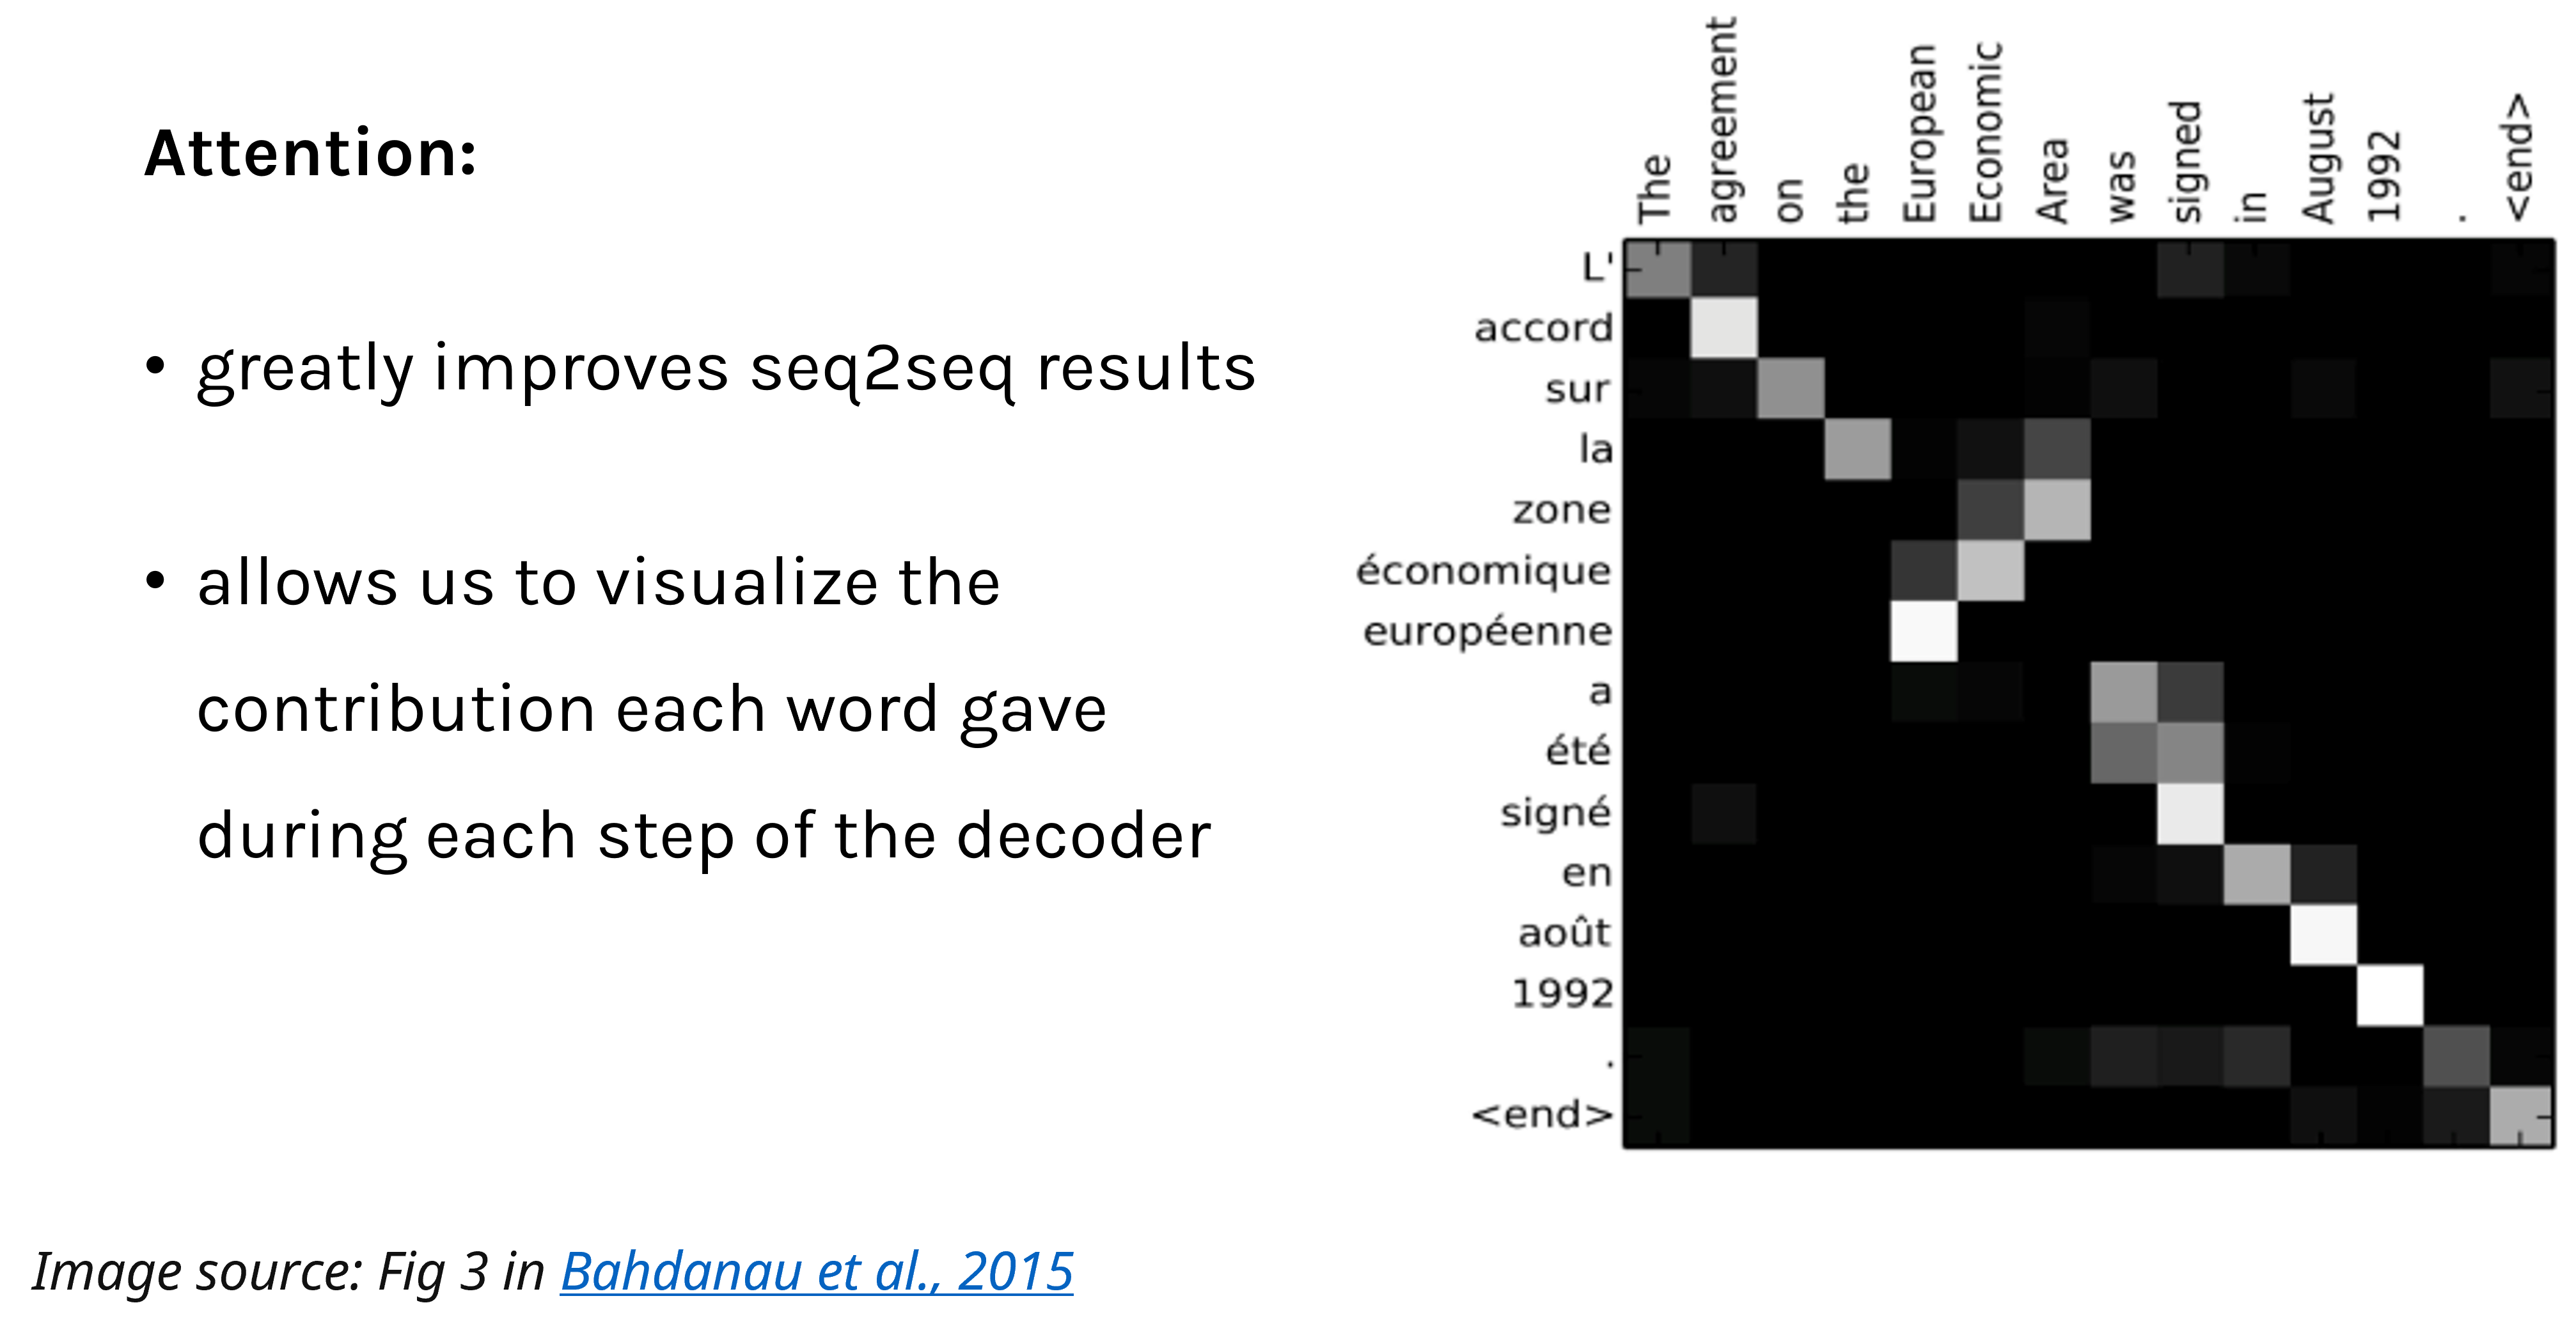
\includegraphics[width=\linewidth,keepaspectratio]{bert32}
\end{center}	

\end{frame}

%%%%%%%%%%%%%%%%%%%%%%%%%%%%%%%%%%%%%%%%%%%%%%%%%%%%%%%%%%%%%%%%%%%%%%%%%%%%%%%%%%
\begin{frame}[fragile]\frametitle{}
\begin{center}
{\Large Embeddings}
\end{center}
\end{frame}

%%%%%%%%%%%%%%%%%%%%%%%%%%%%%%%%%%%%%%%%%%%%%%%%%%%%%%%%%%%
\begin{frame}[fragile]\frametitle{ELMo: Embeddings from Language  Models}

Deep contextualized word representations. Peters et al. NAACL 2018.  https://arxiv.org/abs/1802.05365

\begin{itemize}
\item ``Instead of using a fixed embedding for each word, ELMo looks at the entire sentence before assigning each word in it an embedding.''
\item Breakout version of word token vectors or
contextual word vectors
\item Learn word token vectors using long contexts not context  windows (here, whole sentence, could be longer)
\item Learn a deep Bi-NLM and use all its layers in prediction
\end{itemize}

{\tiny (Ref: CS224n: Natural Language Processing with Deep Learning - Christopher Manning)}

\end{frame}

%%%%%%%%%%%%%%%%%%%%%%%%%%%%%%%%%%%%%%%%%%%%%%%%%%%%%%%%%%%
\begin{frame}[fragile]\frametitle{ELMo: Embeddings from Language  Models}

\begin{itemize}
\item Train a bidirectional LM
\item Aim at performant but not overly large LM:

\begin{itemize}
\item Use 2 biLSTM layers
\item Use character CNN to build initial word representation 
\item User 4096 dim hidden/cell LSTM states with 512 dim projections to next input
\item Use a residual connection
\item Tie parameters of token input and output (softmax) and tie these between forward and backward LMs
\end{itemize}

\end{itemize}

{\tiny (Ref: CS224n: Natural Language Processing with Deep Learning - Christopher Manning)}

\end{frame}

%%%%%%%%%%%%%%%%%%%%%%%%%%%%%%%%%%%%%%%%%%%%%%%%%%%%%%%%%%%
\begin{frame}[fragile]\frametitle{ELMo used in a sequence tagger}

\begin{center}
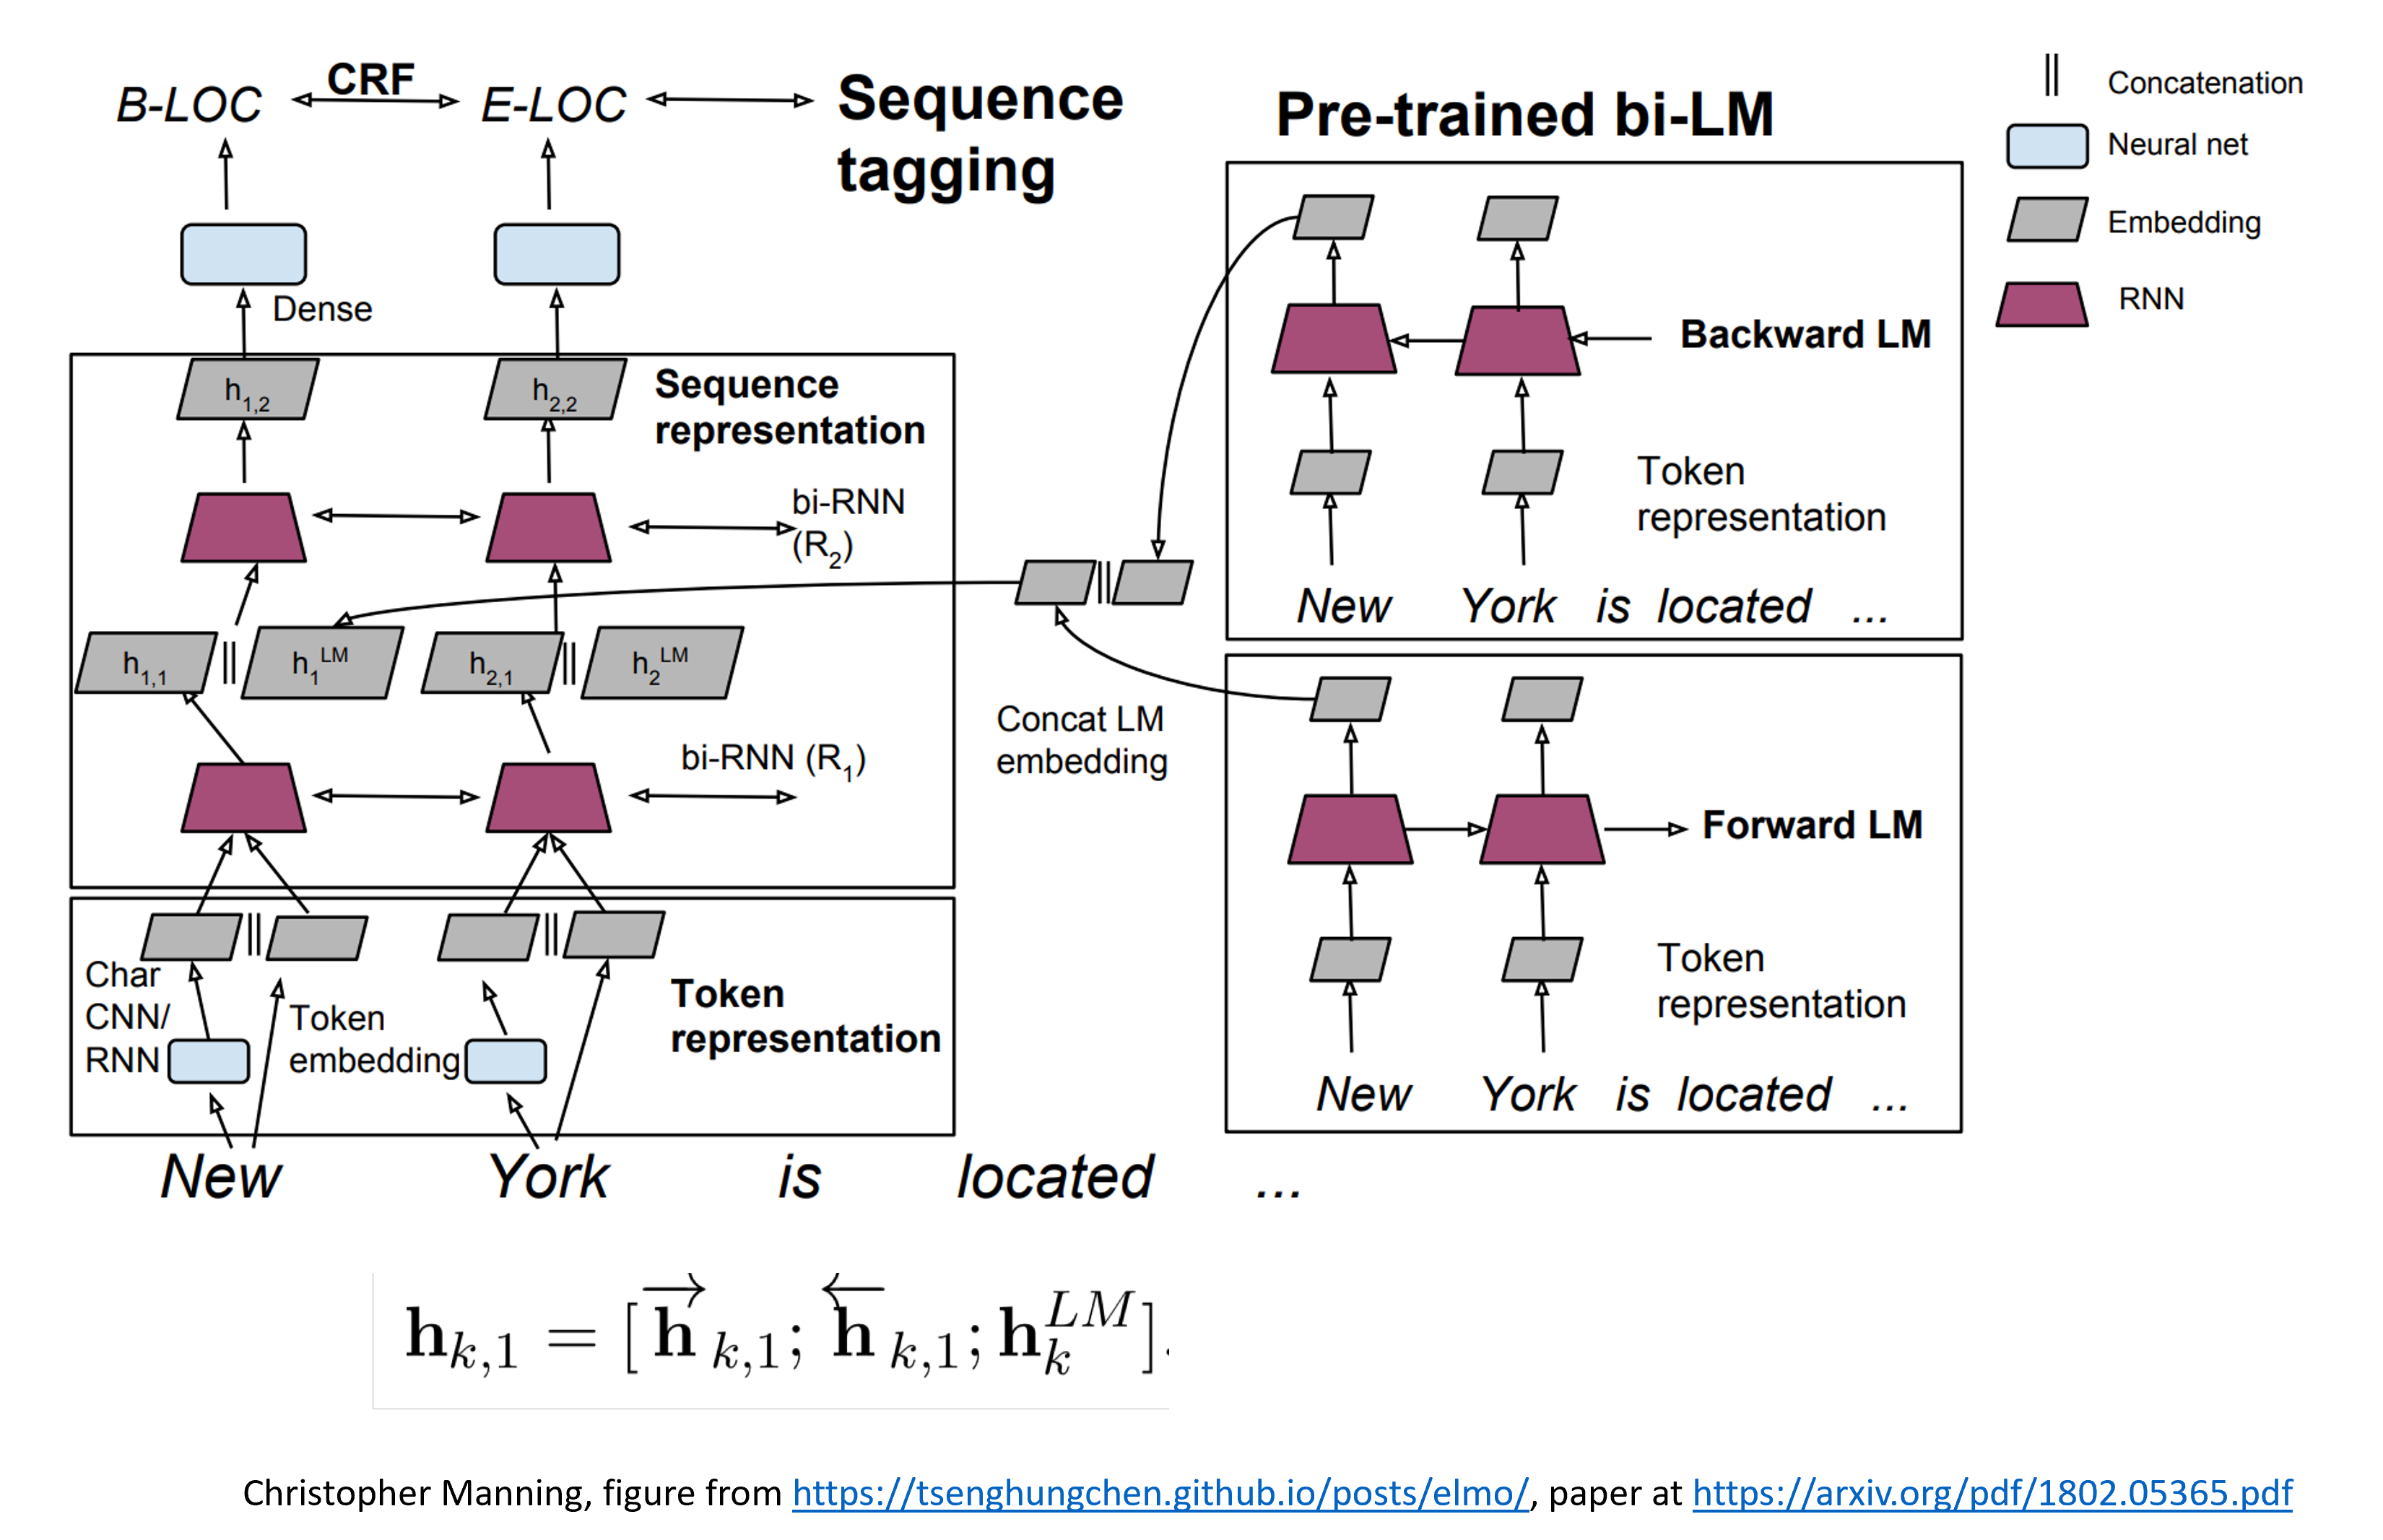
\includegraphics[width=\linewidth,keepaspectratio]{bert33}
\end{center}	

{\tiny (Ref: CS224n: Natural Language Processing with Deep Learning - Christopher Manning)}

\end{frame}

%%%%%%%%%%%%%%%%%%%%%%%%%%%%%%%%%%%%%%%%%%%%%%%%%%%%%%%%%%%
\begin{frame}[fragile]\frametitle{ELMo results: Great for all tasks}

\begin{center}
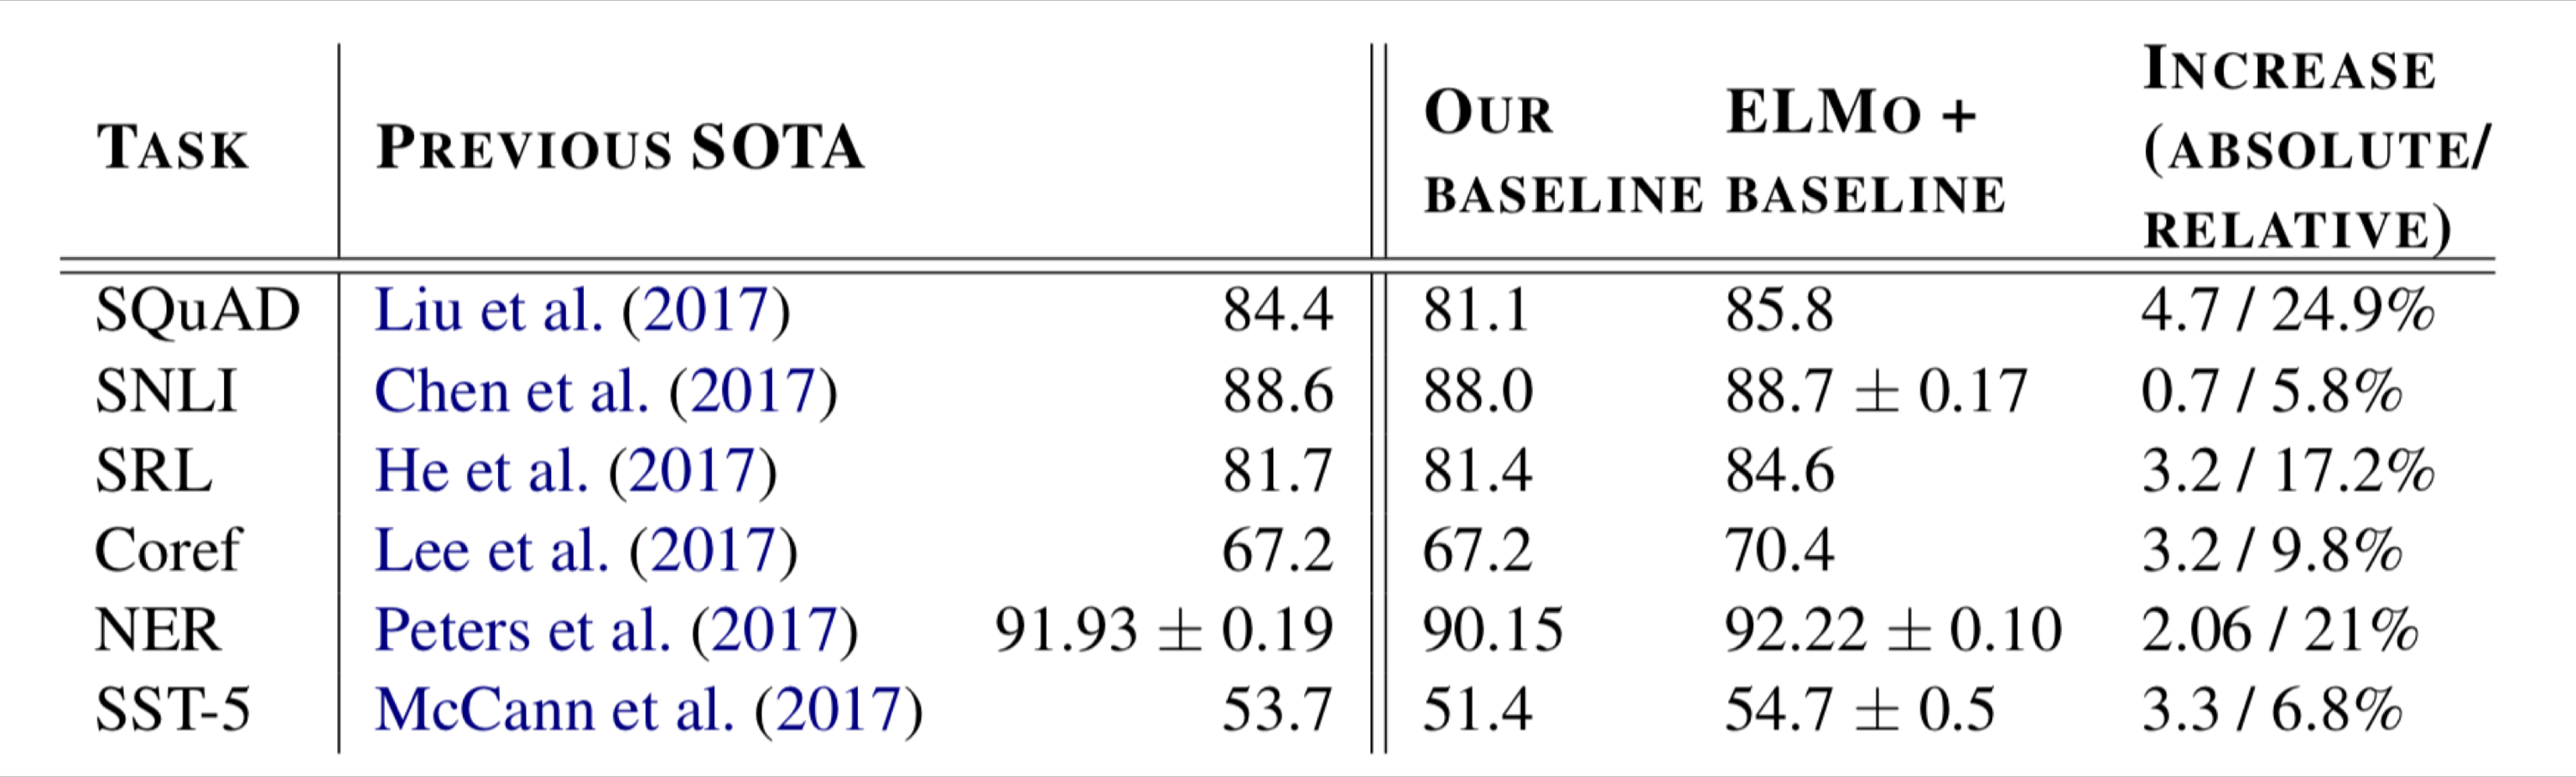
\includegraphics[width=\linewidth,keepaspectratio]{bert34}
\end{center}	

{\tiny (Ref: CS224n: Natural Language Processing with Deep Learning - Christopher Manning)}

\end{frame}

%%%%%%%%%%%%%%%%%%%%%%%%%%%%%%%%%%%%%%%%%%%%%%%%%%%%%%%%%%%
\begin{frame}[fragile]\frametitle{ELMo: Roles of different layers}

The two biLSTM NLM layers have differentiated uses/meanings

\begin{itemize}
\item Lower layer is better for lower-level syntax, etc.
Part-of-speech tagging, syntactic dependencies, NER
\item Higher layer is better for higher-level semantics
Sentiment, Semantic role labeling, question answering, SNLI

\end{itemize}


{\tiny (Ref: CS224n: Natural Language Processing with Deep Learning - Christopher Manning)}

\end{frame}

%%%%%%%%%%%%%%%%%%%%%%%%%%%%%%%%%%%%%%%%%%%%%%%%%%%%%%%%%%%
\begin{frame}[fragile]\frametitle{Issues with recurrent models: Linear interaction distance}

O(sequence length) steps for distant word pairs to interact means:

\begin{itemize}
\item Hard to learn long-distance dependencies (because gradient problems!)
\item Linear order of words is ``baked in''; not necessarily the  right way to think about sentences \ldots
\end{itemize}	 

\begin{center}
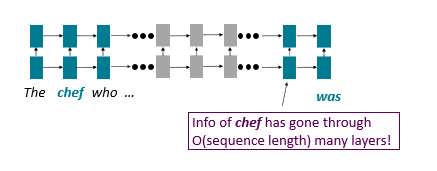
\includegraphics[width=\linewidth,keepaspectratio]{bert35}
\end{center}	

 
{\tiny (Ref: Language \& Machine Learning - John Hewitt)}
\end{frame}

%%%%%%%%%%%%%%%%%%%%%%%%%%%%%%%%%%%%%%%%%%%%%%%%%%%%%%%%%%%
\begin{frame}[fragile]\frametitle{Issues with recurrent models: Lack of parallelizability}

Forward and backward passes have O(sequence length) unparallelizable operations

\begin{itemize}
\item GPUs can perform a bunch of independent computations at once!
\item But future RNN hidden states can’t be computed in full before past RNN
hidden states have been computed
\item Inhibits training on very large datasets!
\end{itemize}	 

\begin{center}
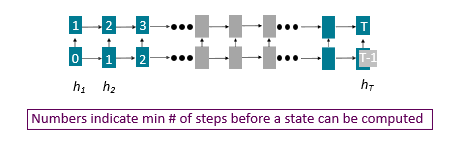
\includegraphics[width=\linewidth,keepaspectratio]{bert36}
\end{center}	

 
{\tiny (Ref: Language \& Machine Learning - John Hewitt)}
\end{frame}

%%%%%%%%%%%%%%%%%%%%%%%%%%%%%%%%%%%%%%%%%%%%%%%%%%%%%%%%%%%
\begin{frame}[fragile]\frametitle{If not recurrence, then what? How about word windows?}

Word window models aggregate local contexts

\begin{itemize}
\item Also known as 1D convolution
\item Number of unparallelizable operations not tied to sequence length!
\end{itemize}	 

\begin{center}
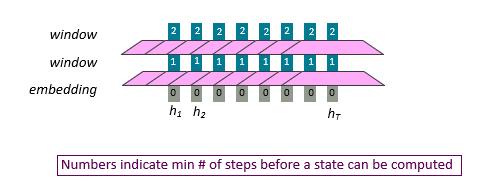
\includegraphics[width=\linewidth,keepaspectratio]{bert37}
\end{center}	

 
{\tiny (Ref: Language \& Machine Learning - John Hewitt)}
\end{frame}

%%%%%%%%%%%%%%%%%%%%%%%%%%%%%%%%%%%%%%%%%%%%%%%%%%%%%%%%%%%
\begin{frame}[fragile]\frametitle{If not recurrence, then what? How about word windows?}

What about long-distance dependencies?

\begin{itemize}
\item Stacking word window layers allows interaction between farther words
\item But if your sequences are too long, you’ll just ignore long-distance context

\end{itemize}	 

\begin{center}
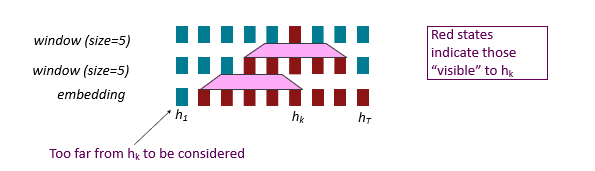
\includegraphics[width=\linewidth,keepaspectratio]{bert38}
\end{center}	

 
{\tiny (Ref: Language \& Machine Learning - John Hewitt)}
\end{frame}

%%%%%%%%%%%%%%%%%%%%%%%%%%%%%%%%%%%%%%%%%%%%%%%%%%%%%%%%%%%
\begin{frame}[fragile]\frametitle{If not recurrence, then what? How about attention?}


\begin{itemize}
\item Attention treats each word’s representation as a query to access and  incorporate information from a set of values.
\item We saw attention from the decoder to the encoder; today we’ll think about
attention within a single sentence.
\item If attention gives us access to any state… maybe we can just use attention and don’t need the RNN?
\item Number of unparallelizable operations not tied to sequence length.
\item All words interact at every layer!

\end{itemize}	 

\begin{center}
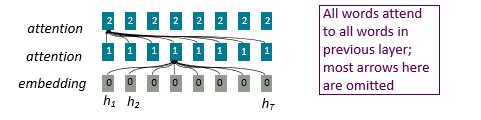
\includegraphics[width=\linewidth,keepaspectratio]{bert39}
\end{center}	

 
{\tiny (Ref: Language \& Machine Learning - John Hewitt)}
\end{frame}

%%%%%%%%%%%%%%%%%%%%%%%%%%%%%%%%%%%%%%%%%%%%%%%%%%%%%%%%%%%
\begin{frame}[fragile]\frametitle{Self-Attention}


\begin{center}
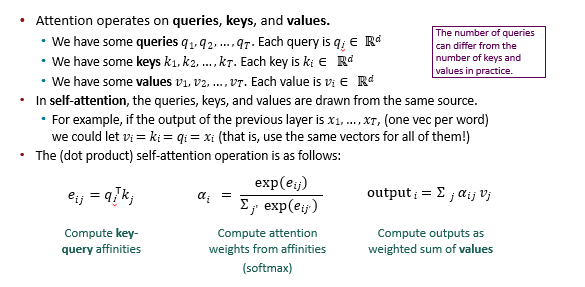
\includegraphics[width=\linewidth,keepaspectratio]{bert40}
\end{center}	

 
{\tiny (Ref: Language \& Machine Learning - John Hewitt)}
\end{frame}

%%%%%%%%%%%%%%%%%%%%%%%%%%%%%%%%%%%%%%%%%%%%%%%%%%%%%%%%%%%
\begin{frame}[fragile]\frametitle{Self-Attention}


\begin{center}
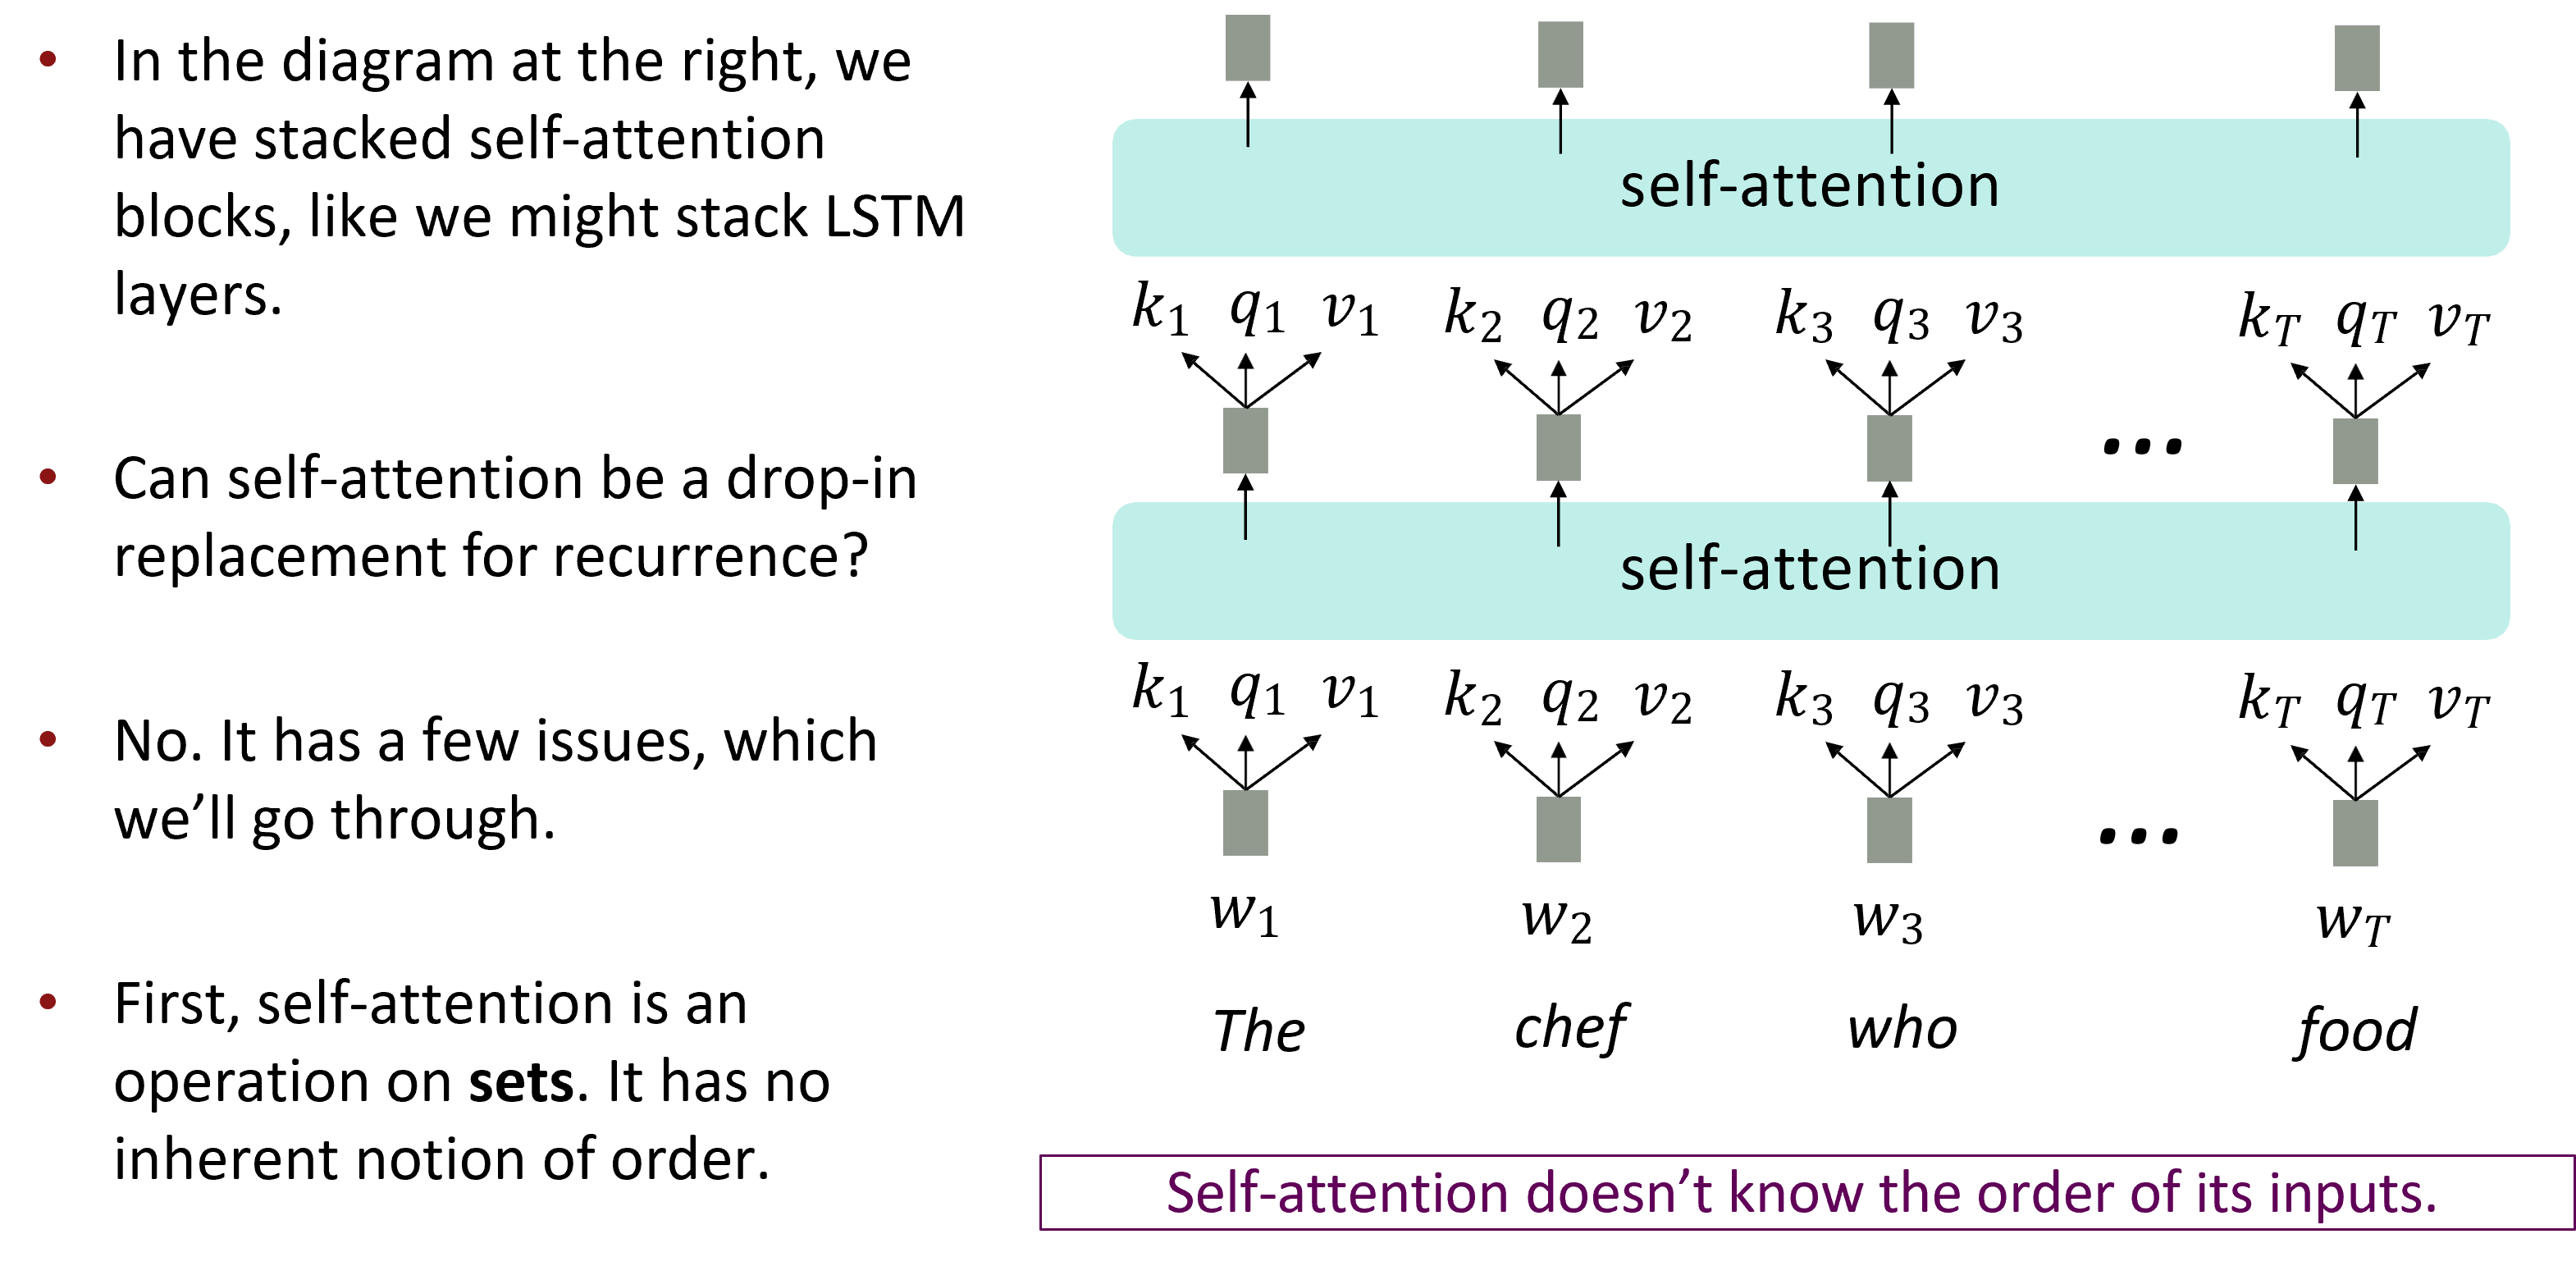
\includegraphics[width=\linewidth,keepaspectratio]{bert41}
\end{center}	

 
{\tiny (Ref: Language \& Machine Learning - John Hewitt)}
\end{frame}

%%%%%%%%%%%%%%%%%%%%%%%%%%%%%%%%%%%%%%%%%%%%%%%%%%%%%%%%%%%
\begin{frame}[fragile]\frametitle{Self-Attention}

Barriers and solutions for Self-Attention as a building block

\begin{center}
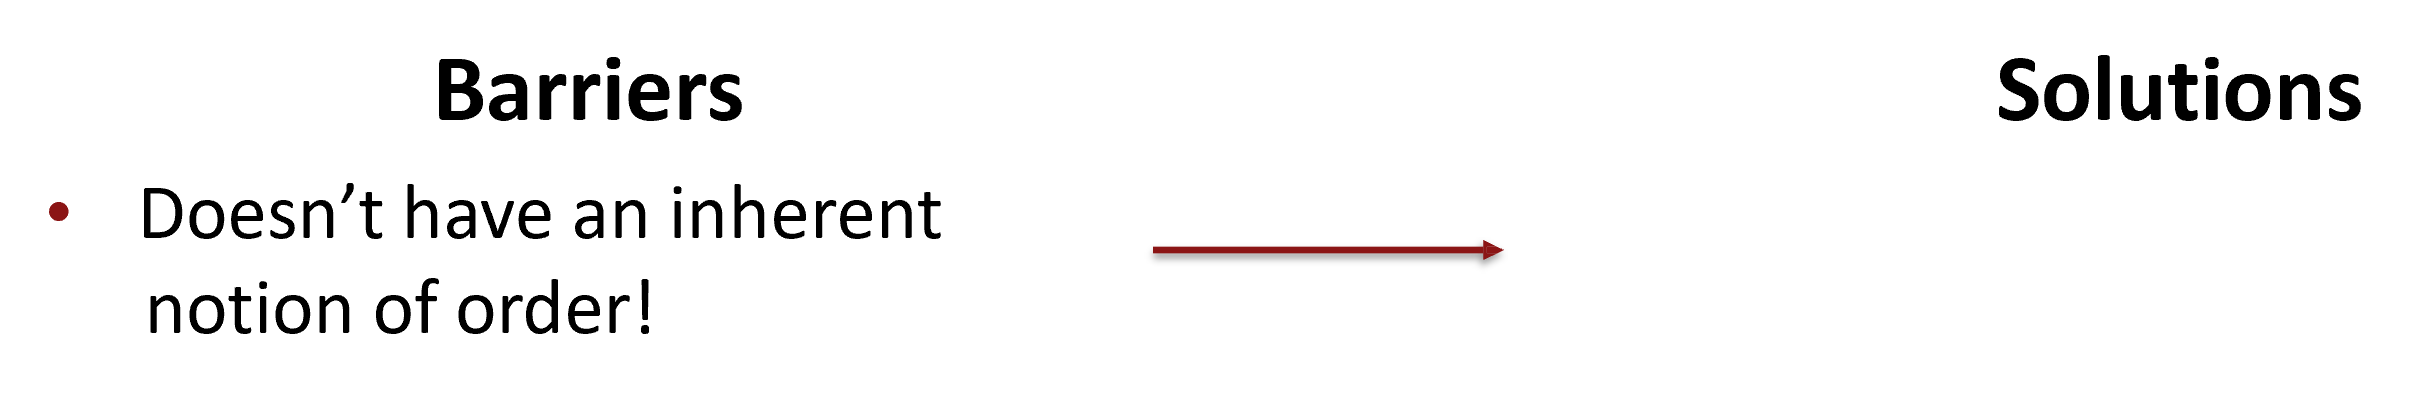
\includegraphics[width=\linewidth,keepaspectratio]{bert42}
\end{center}	

 
{\tiny (Ref: Language \& Machine Learning - John Hewitt)}
\end{frame}

%%%%%%%%%%%%%%%%%%%%%%%%%%%%%%%%%%%%%%%%%%%%%%%%%%%%%%%%%%%
\begin{frame}[fragile]\frametitle{Self-Attention}

Fixing the first self-attention problem: Sequence order

\begin{center}
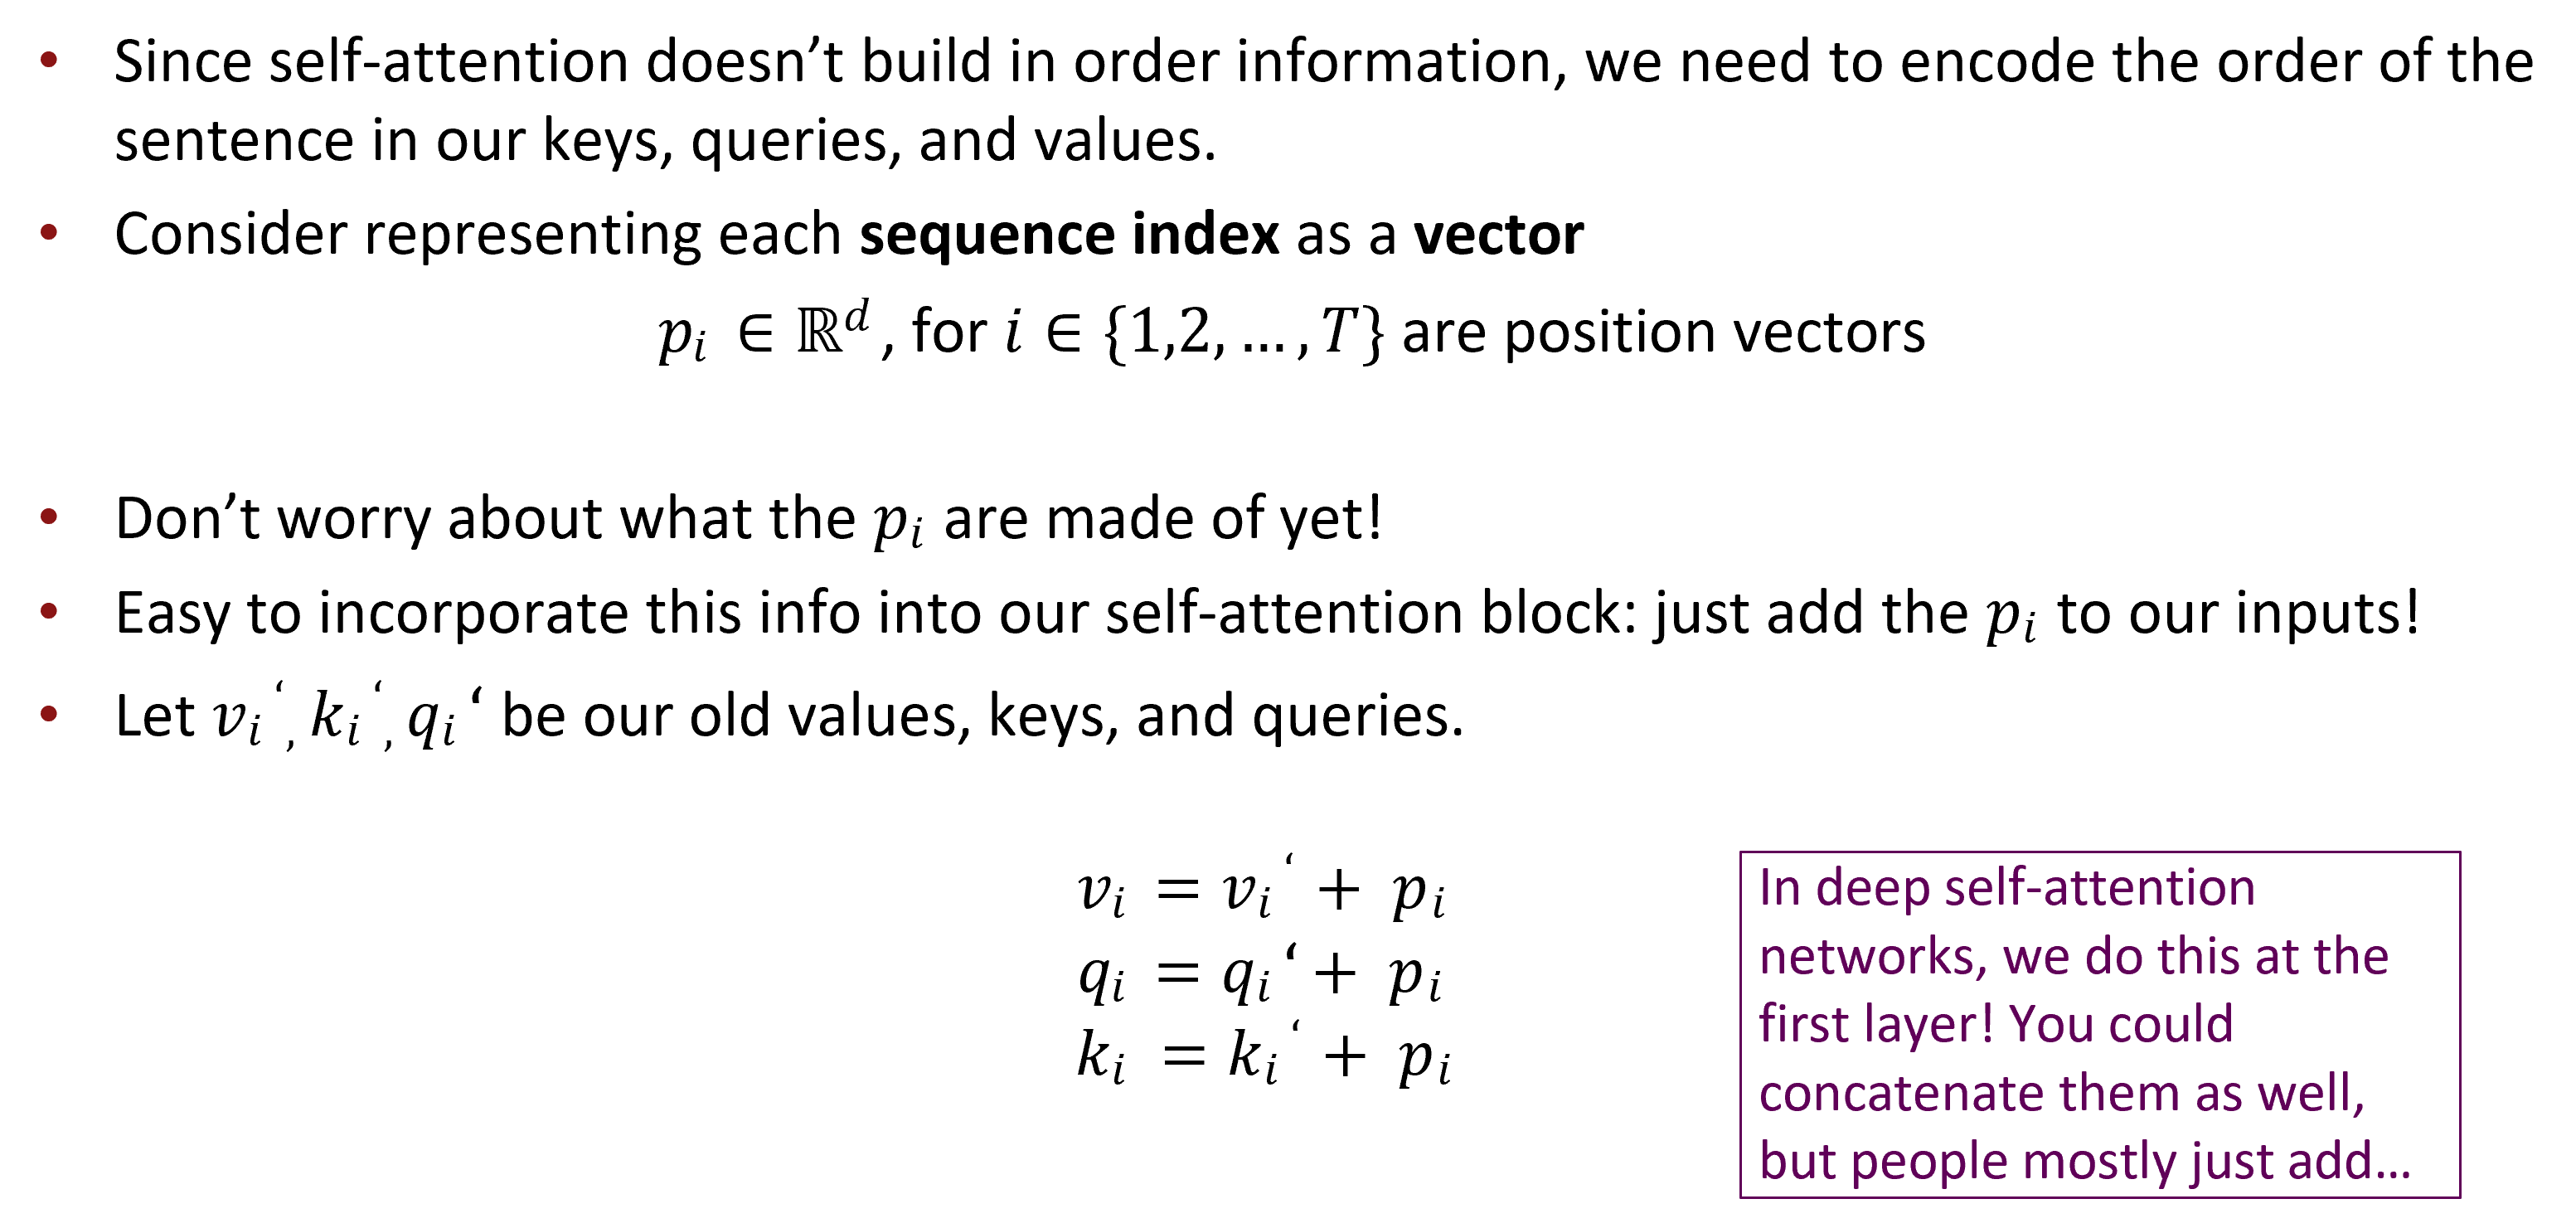
\includegraphics[width=\linewidth,keepaspectratio]{bert43}
\end{center}	

 
{\tiny (Ref: Language \& Machine Learning - John Hewitt)}
\end{frame}

%%%%%%%%%%%%%%%%%%%%%%%%%%%%%%%%%%%%%%%%%%%%%%%%%%%%%%%%%%%
\begin{frame}[fragile]\frametitle{Self-Attention}

Position representation vectors through sinusoids

\begin{center}
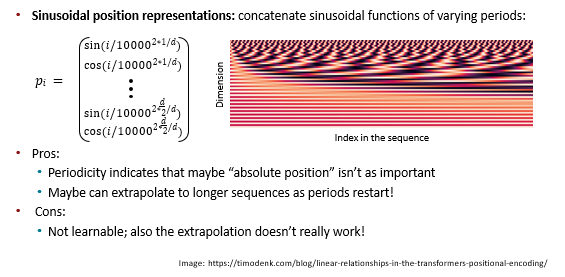
\includegraphics[width=\linewidth,keepaspectratio]{bert44}
\end{center}	

 
{\tiny (Ref: Language \& Machine Learning - John Hewitt)}
\end{frame}

%%%%%%%%%%%%%%%%%%%%%%%%%%%%%%%%%%%%%%%%%%%%%%%%%%%%%%%%%%%
\begin{frame}[fragile]\frametitle{Self-Attention}

Barriers and solutions for Self-Attention as a building block

\begin{center}
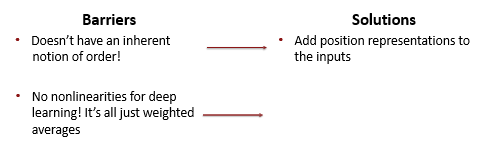
\includegraphics[width=\linewidth,keepaspectratio]{bert45}
\end{center}	

 
{\tiny (Ref: Language \& Machine Learning - John Hewitt)}
\end{frame}

%%%%%%%%%%%%%%%%%%%%%%%%%%%%%%%%%%%%%%%%%%%%%%%%%%%%%%%%%%%
\begin{frame}[fragile]\frametitle{Self-Attention}

Adding nonlinearities in self-attention

\begin{center}
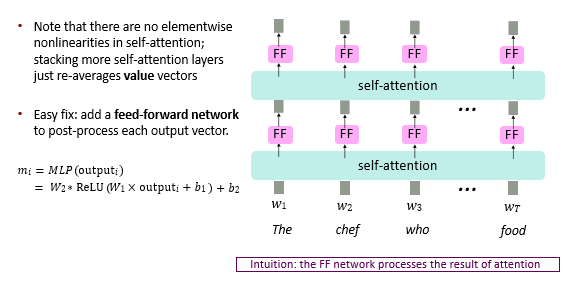
\includegraphics[width=\linewidth,keepaspectratio]{bert46}
\end{center}	

 
{\tiny (Ref: Language \& Machine Learning - John Hewitt)}
\end{frame}

%%%%%%%%%%%%%%%%%%%%%%%%%%%%%%%%%%%%%%%%%%%%%%%%%%%%%%%%%%%
\begin{frame}[fragile]\frametitle{Self-Attention}

Barriers and solutions for Self-Attention as a building block

\begin{center}
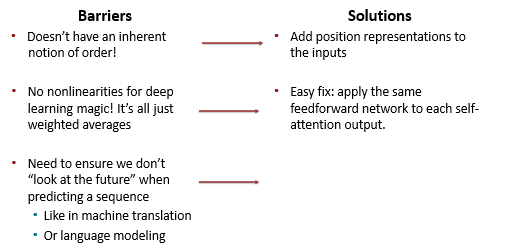
\includegraphics[width=\linewidth,keepaspectratio]{bert47}
\end{center}	

 
{\tiny (Ref: Language \& Machine Learning - John Hewitt)}
\end{frame}


%%%%%%%%%%%%%%%%%%%%%%%%%%%%%%%%%%%%%%%%%%%%%%%%%%%%%%%%%%%
\begin{frame}[fragile]\frametitle{Self-Attention}

Masking the future in self-attention

\begin{center}
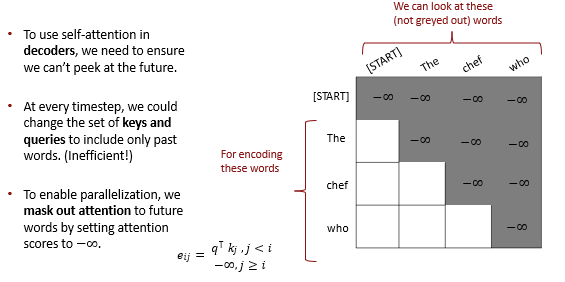
\includegraphics[width=\linewidth,keepaspectratio]{bert48}
\end{center}	

 
{\tiny (Ref: Language \& Machine Learning - John Hewitt)}
\end{frame}

%%%%%%%%%%%%%%%%%%%%%%%%%%%%%%%%%%%%%%%%%%%%%%%%%%%%%%%%%%%
\begin{frame}[fragile]\frametitle{Self-Attention}

Barriers and solutions for Self-Attention as a building block

\begin{center}
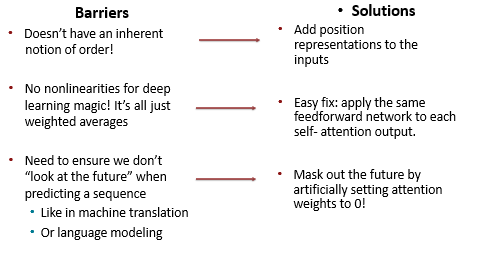
\includegraphics[width=\linewidth,keepaspectratio]{bert49}
\end{center}	

 
{\tiny (Ref: Language \& Machine Learning - John Hewitt)}
\end{frame}

%%%%%%%%%%%%%%%%%%%%%%%%%%%%%%%%%%%%%%%%%%%%%%%%%%%%%%%%%%%
\begin{frame}[fragile]\frametitle{Self-Attention}

Necessities for a self-attention building block:

\begin{itemize}
\item Self-attention:
the basis of the method.
\item Position representations:
Specify the sequence order, since self-attention is an unordered function of its  inputs.
\item Nonlinearities:
\begin{itemize}
\item At the output of the self-attention block
\item Frequently implemented as a simple feed-forward network.
\end{itemize}	 

\item Masking:
\begin{itemize}
\item In order to parallelize operations while not looking at the future.
\item Keeps information about the future from “leaking” to the past.
\end{itemize}	 

\item That’s it! But this is not the Transformer model we’ve been hearing about.


\end{itemize}	 

 
{\tiny (Ref: Language \& Machine Learning - John Hewitt)}
\end{frame}

%%%%%%%%%%%%%%%%%%%%%%%%%%%%%%%%%%%%%%%%%%%%%%%%%%%%%%%%%%%%%%%%%%%%%%%%%%%%%%%%%%
\begin{frame}[fragile]\frametitle{}
\begin{center}
{\Large Transformer \\ \small Attention is all you need}
\end{center}
\end{frame}



%%%%%%%%%%%%%%%%%%%%%%%%%%%%%%%%%%%%%%%%%%%%%%%%%%%%%%%%%%%%%%%%%%%%%%%%%%%%%%%%%%
\begin{frame}[fragile]\frametitle{}
\begin{center}
{\Large End}
\end{center}
\end{frame}


%%%%%%%%%%%%%%%%%%%%%%%%%%%%%%%%%%%%%%%%%%%%%%%%%%%%%%%%%%%
\begin{frame}[fragile]\frametitle{Scratch Notes}

\begin{itemize}
\item Transformer as architecture: No recurrence but attention
\item Attention is softmax output fed back in each iteration
\item Goal of masking task is to learn language, ie features, actual task need small supervised data for finetuning  stored as pre-training

\end{itemize}
	  
\end{frame}

%%%%%%%%%%%%%%%%%%%%%%%%%%%%%%%%%%%%%%%%%%%%%%%%%%%%%%%%%%%
\begin{frame}[fragile]\frametitle{Reference}

\begin{itemize}
\item CS224n: Natural Language Processing with Deep Learning - Christopher Manning
\end{itemize}
	  
\end{frame}

% %%%%%%%%%%%%%%%%%%%%%%%%%%%%%%%%%%%%%%%%%%%%%%%%%%%%%%%%%%%
% \begin{frame}[fragile]\frametitle{Sample List Slide}

% \begin{itemize}
% \item aaa
% \end{itemize}
	  
% \end{frame}

% %%%%%%%%%%%%%%%%%%%%%%%%%%%%%%%%%%%%%%%%%%%%%%%%%%%%%%%%%%%
% \begin{frame}[fragile]\frametitle{Sample Picture Inclusion}

% \begin{center}
% \includegraphics[width=0.8\linewidth,keepaspectratio]{myphoto}
% \end{center}	  
% \end{frame}

% %%%%%%%%%%%%%%%%%%%%%%%%%%%%%%%%%%%%%%%%%%%%%%%%%%%
% \begin{frame}[fragile] \frametitle{Sample Code Listing}
% \begin{lstlisting}
% import aaa
% \end{lstlisting}

% \end{frame}

% %%%%%%%%%%%%%%%%%%%%%%%%%%%%%%%%%%%%%%%%%%%%%%%%%%%%%%%%%%%
% \begin{frame}[fragile]\frametitle{Sample Two Columns Slide}
% \begin{columns}
    % \begin{column}[T]{0.6\linewidth}
      % \begin{itemize}
		% \item aaa
	  % \end{itemize}

    % \end{column}
    % \begin{column}[T]{0.4\linewidth}
      % \begin{itemize}
		% \item bbb
	  % \end{itemize}
    % \end{column}
  % \end{columns}
% \end{frame}

% %%%%%%%%%%%%%%%%%%%%%%%%%%%%%%%%%%%%%%%%%%%%%%%%%%%%%%%%%%%%%%%%%%%%%%%%%%%%%%%%%%%
% \begin{frame}[fragile]\frametitle{Sample Tabular Data}

% aaa

% \begin{tabular}{|c|c|}
	% \hline
	% Platform & Time (s) \\
	% \hline \hline
	% Python & $\sim$1500.0 \\
	% \hline
	% NumPy & 29.3 \\
	% \hline
	% Matlab & $\sim$29.0 \\
	% \hline
	% Octave & $\sim$60.0 \\
	% \hline
	% Blitz (C++) & 9.5 \\
	% \hline
	% Fortran & 2.5 \\
	% \hline
	% C & 2.2 \\
	% \hline
% \end{tabular}

% \end{frame}
